\documentclass[french,A4paper,]{book}
\usepackage[ED=EDSYS-Robo, Ets=INSA]{tlsflyleaf}
\usepackage{algpseudocode}
\usepackage{algorithm}
\usepackage{bm}
\algnewcommand{\Commente}[1]{\hfill #1}
\usepackage{lmodern}
\usepackage{amssymb,amsmath}
\usepackage{ifxetex,ifluatex}
\usepackage{fixltx2e} % provides \textsubscript
\ifnum 0\ifxetex 1\fi\ifluatex 1\fi=0 % if pdftex
  \usepackage[T1]{fontenc}
  \usepackage[utf8]{inputenc}
  \DeclareUnicodeCharacter{2011}{\nobreakdash}
\else % if luatex or xelatex
  \usepackage{unicode-math}
  \defaultfontfeatures{Ligatures=TeX,Scale=MatchLowercase}
\fi
% use upquote if available, for straight quotes in verbatim environments
\IfFileExists{upquote.sty}{\usepackage{upquote}}{}
% use microtype if available
\IfFileExists{microtype.sty}{%
\usepackage[]{microtype}
\UseMicrotypeSet[protrusion]{basicmath} % disable protrusion for tt fonts
}{}
\PassOptionsToPackage{hyphens}{url} % url is loaded by hyperref
\usepackage[unicode=true]{hyperref}
\hypersetup{
            pdftitle={Génération de mouvement en robotique mobile et humanoïde},
            pdfauthor={Guilhem Saurel},
            pdfborder={0 0 0},
            breaklinks=true}
\urlstyle{same}  % don't use monospace font for urls
\ifnum 0\ifxetex 1\fi\ifluatex 1\fi=0 % if pdftex
  \usepackage[shorthands=off,main=french]{babel}
\else
  \usepackage{polyglossia}
  \setmainlanguage[]{french}
\fi
\usepackage{longtable,booktabs}
% Fix footnotes in tables (requires footnote package)
\IfFileExists{footnote.sty}{\usepackage{footnote}\makesavenoteenv{long table}}{}
\usepackage{graphicx,grffile}
\makeatletter
\def\maxwidth{\ifdim\Gin@nat@width>\linewidth\linewidth\else\Gin@nat@width\fi}
\def\maxheight{\ifdim\Gin@nat@height>\textheight\textheight\else\Gin@nat@height\fi}
\makeatother
% Scale images if necessary, so that they will not overflow the page
% margins by default, and it is still possible to overwrite the defaults
% using explicit options in \includegraphics[width, height, ...]{}
\setkeys{Gin}{width=\maxwidth,height=\maxheight,keepaspectratio}
\IfFileExists{parskip.sty}{%
\usepackage{parskip}
}{% else
\setlength{\parindent}{0pt}
\setlength{\parskip}{6pt plus 2pt minus 1pt}
}
\setlength{\emergencystretch}{3em}  % prevent overfull lines
\providecommand{\tightlist}{%
  \setlength{\itemsep}{0pt}\setlength{\parskip}{0pt}}
\setcounter{secnumdepth}{5}
% Redefines (sub)paragraphs to behave more like sections
\ifx\paragraph\undefined\else
\let\oldparagraph\paragraph
\renewcommand{\paragraph}[1]{\oldparagraph{#1}\mbox{}}
\fi
\ifx\subparagraph\undefined\else
\let\oldsubparagraph\subparagraph
\renewcommand{\subparagraph}[1]{\oldsubparagraph{#1}\mbox{}}
\fi

% set default figure placement to htbp
\makeatletter
\def\fps@figure{htbp}
\makeatother

\usepackage{subfig}
\AtBeginDocument{%
\renewcommand*\figurename{Figure}
\renewcommand*\tablename{Table}
}
\AtBeginDocument{%
\renewcommand*\listfigurename{List of Figures}
\renewcommand*\listtablename{List of Tables}
}
\usepackage{float}
\floatstyle{ruled}
\makeatletter
\@ifundefined{c@chapter}{\newfloat{codelisting}{h}{lop}}{\newfloat{codelisting}{h}{lop}[chapter]}
\makeatother
\floatname{codelisting}{Listing}
\newcommand*\listoflistings{\listof{codelisting}{List of Listings}}

\title{Génération de mouvement en robotique mobile et humanoïde}
\author{Guilhem Saurel}
\providecommand{\institute}[1]{}
\institute{LAAS-CNRS}
\date{}

\defencedate{29 septembre 2017}
\lab{Laboratoire d'Analyse et d'Architecture des Systèmes LAAS-CNRS}
\nboss{1}
\makesomeone{boss}{1}{Jean-Paul Laumond}{}{}
\nreferee{2}
\makesomeone{referee}{1}{Brigitte D'Andrea-Novel}{}{}
\makesomeone{referee}{2}{Christine Chevallereau}{}{}
\njudge{6}
\makesomeone{judge}{1}{Philippe Souères}{Directeur de Recherche}{Présdent du Jury}
\makesomeone{judge}{2}{Brigitte D'Andrea-Novel}{Professeur}{Membre du Jury}
\makesomeone{judge}{3}{Christine Chevallereau}{Directeur de Recherche}{Membre du Jury}
\makesomeone{judge}{4}{Jean-Paul Laumond}{Directeur de Recherche}{Membre du Jury}
\makesomeone{judge}{5}{Michel Taïx}{Maître de Conférences}{Membre du Jury}
\makesomeone{judge}{6}{Guy Caverot}{Ingénieur, Ph.D.}{Invité}

\pagestyle{fancy}

\begin{document}
\makeflyleaf

{
\setcounter{tocdepth}{2}
\tableofcontents
}

\renewcommand{\listtablename}{Liste des Tables}
\renewcommand{\listfigurename}{Liste des Figures}
\renewcommand{\listalgorithmname}{Liste des Algorithmes}

\listoftables
\listoffigures
\listofalgorithms
\renewcommand{\thechapter}{\Alph{chapter}}
\renewcommand{\theequation}{\Alph{chapter}-\arabic{equation}}

\makeatletter
\renewcommand{\ALG@name}{Algorithme} \makeatother
\algnewcommand\Ands{\;\textbf{and}\;}
\algnewcommand\Ors{\;\textbf{or}\;}

\newcommand{\vectwo}[2]{\ensuremath{\left(\begin{array}{c}{#1} \\ {#2}\end{array}\right)}}

\fancyhead{} \fancyfoot{} \fancyhead[LE]{\thepage}
\fancyhead[RO]{\thepage} \fancyhead[RE]{\leftmark}
\fancyhead[LO]{\rightmark}

\chapter{Introduction}\label{introduction}

Il présente dans un premier temps la robotique par son histoire, ses
applications, et sa place dans la société dans la sec.~\ref{sec:intgen},
et donne des précautions d'usage dans la sec.~\ref{sec:precautions}.

Il décrit enfin le plan du reste de cette thèse et ses contributions
respectivement dans les secs.~\ref{sec:plan}, \ref{sec:contributions}.

\section{Introduction Générale}\label{sec:intgen}

La robotique consiste à augmenter l'autonomie d'une machine, en lui
donnant des facultés de perception, de décision et d'action.

Grâce à un savant mélange d'électronique, d'informatique, de mécanique,
de mathématiques, d'intelligence artificielle, et d'automatique, elle a
aujourd'hui bien dépassé le stade de science-fiction, où elle était
encore confinée il y a quelques décennies à peine.

En effet, la culture robotique est antérieure à ses applications
industrielles et à la recherche qui y est associée. Le terme robot
lui-même trouve son origine en 1920 dans une pièce de théâtre
tchécoslovaque de Karel Čapek. Il y désigne un automate travailleur
universel, dans le sens où il pourrait exécuter n'importe quelle tâche.

Le premier automate industriel qui ait vocation a être universel,
Unimate, est un bras manipulateur d'assemblage pour les chaînes de
production de la General Motors, et date des années 1960.

Entre temps, Isaac Asimov a eu le temps d'introduire les «~Trois lois de
la robotique~» dans ses romans de science-fiction dès les années 1940.
Puis, dans les années 1950, les enfants japonais ont à leur tour pu
découvrir la robotique avec le manga «~Astro, le petit robot~» d'Osamu
Tezuka.

Ce manga a initié un nouveau genre, celui des «~Mecha~», mettant en
scène des armures robotisées humanoïdes. De ce genre est par exemple
issu l'univers de Gundam (fig.~\ref{fig:gundam}), une franchise créée
dans les années 1980 comportant entre autres des films, des romans, des
mangas, des animés et des jouets, et générant de nos jours annuellement
environ 50 milliards de yens, soit 500 millions d'euros.

Parmi les artistes qui ont travaillé pour cette franchise, on retrouve
le designer Yutaka Izubuchi, qui a également dessiné la première
véritable plateforme de recherche en robotique humanoïde, HRP-2,
financée par le programme japonais «~Humanoid Robotics Project~».

Suite à la création du JRL (CNRS/AIST), un laboratoire franco-japonais
de robotique, le LAAS-CNRS est le seul laboratoire à disposer d'une
telle plateforme en dehors du Japon, et ce depuis 2006~: il s'agit
d'HRP-2 14 (fig.~\ref{fig:hrp2}).

\begin{figure}
\centering

\hspace*{\fill}
\subfloat[HRP-2 14, au LAAS-CNRS en
2015]{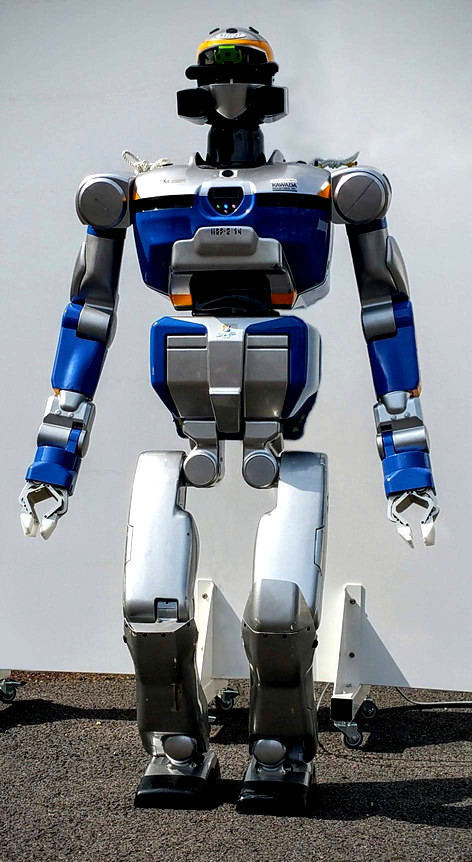
\includegraphics[height=10.00000cm]{imgs/hrp2.jpg}\label{fig:hrp2}}
\hfill%
\subfloat[Statue du Gundam RX-78-2 de taille réelle (18 mètres de haut),
exposée de 2009 à 2017 sur l'île artificielle d'Odaiba à
Tokyo]{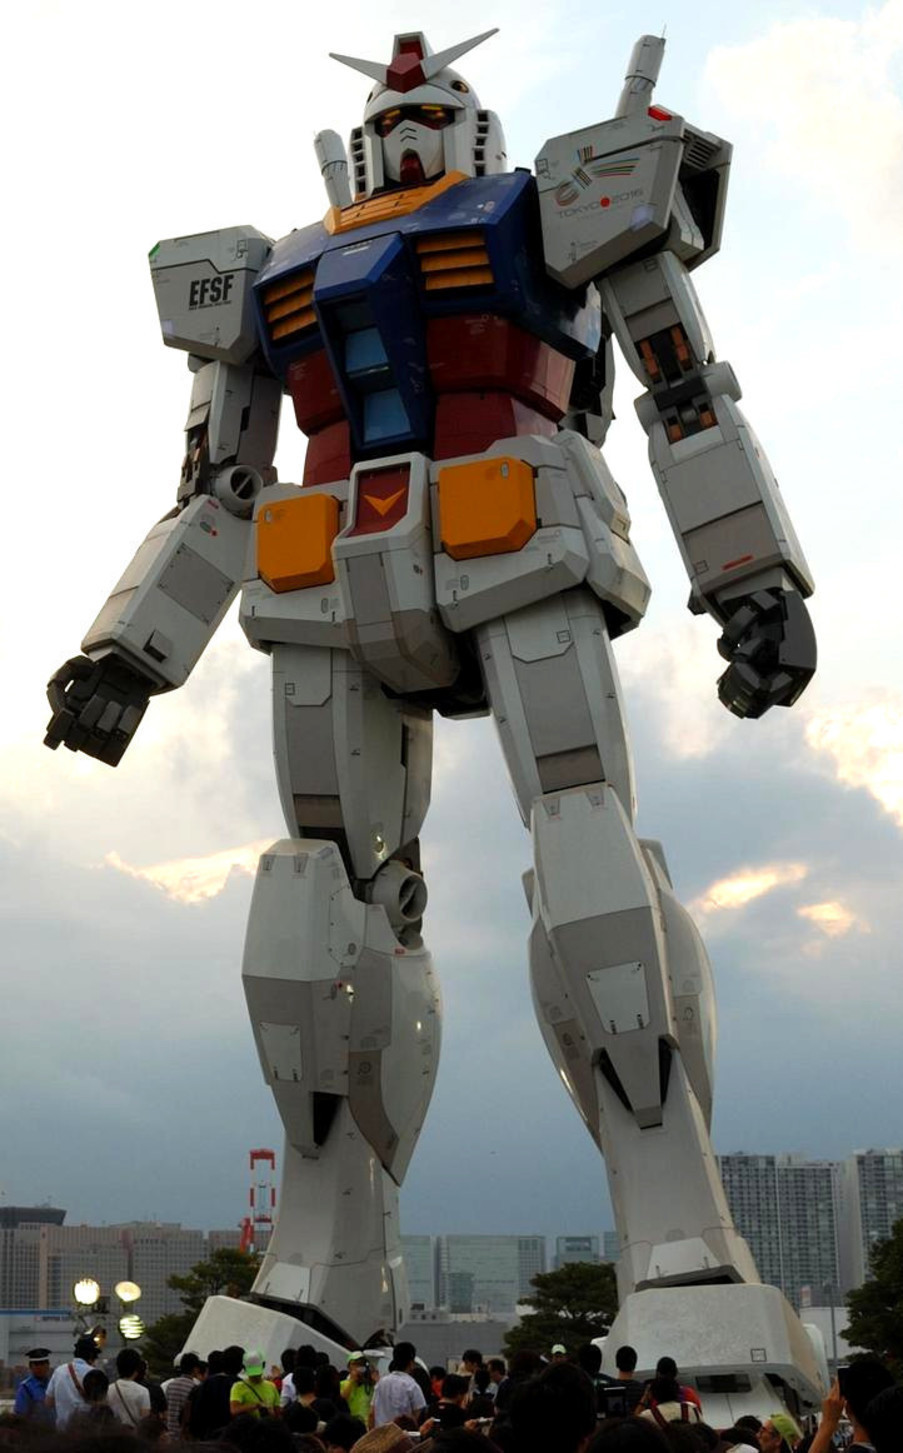
\includegraphics[height=10.00000cm]{imgs/gundam.jpg}\label{fig:gundam}}
\hspace*{\fill}

\caption{Robots humanoïdes japonais, dans la recherche à gauche, et dans
la fiction à droite.}

\label{fig:japon}

\end{figure}

Les robots humanoïdes illustrent bien la robotique dans l'imaginaire,
mais en pratique on trouve des robots à roues dans bien plus
d'applications et depuis bien plus longtemps.

Le robot mobile HILARE (Giralt, Sobek, et Chatila
\protect\hyperlink{ref-giralt79}{1979}) (fig.~\ref{fig:hilare}) a par
exemple été conçu à des fins de recherche au LAAS-CNRS, et a eu trois
version, en 1977, 1990 et 1999.

La recherche en robotique mobile a notamment abouti à la création de
divers rovers lunaires et martiens (fig.~\ref{fig:curiosity}), utilisés
par les scientifiques issus de tous domaines pour réaliser des
expériences dans des conditions inédites, et mieux comprendre notre
système solaire.

Aujourd'hui, de nombreuses entreprises et laboratoire font encore de la
recherche en robotique mobile afin de robotiser nos voitures
(fig.~\ref{fig:googlecar}), et de résoudre ainsi de nombreux problèmes
engendrés par nos moyens de transport classiques.

\begin{figure}
\centering

\hspace*{\fill}
\subfloat[HILARE au musée des Arts et Métiers en
2009]{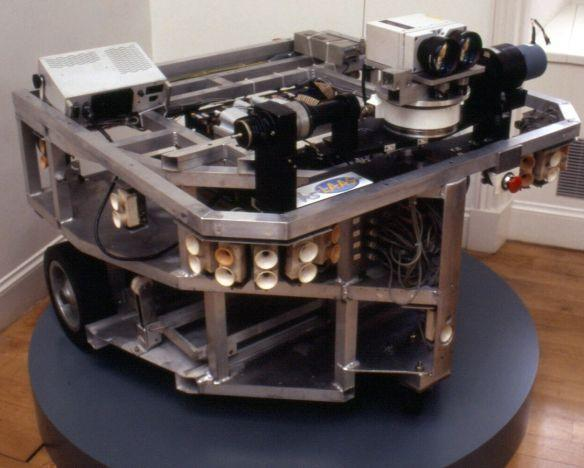
\includegraphics[height=3.00000cm]{imgs/hilare.jpg}\label{fig:hilare}}
\hfill%
\subfloat[Autoportrait de Curiosity sur Mars en
2015]{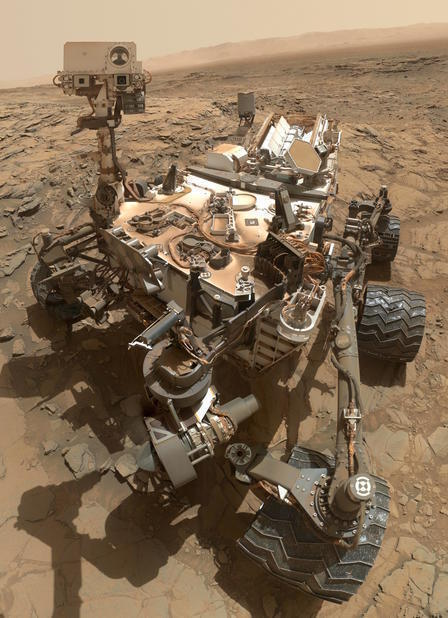
\includegraphics[height=3.00000cm]{imgs/curiosity.jpg}\label{fig:curiosity}}
\hfill%
\subfloat[Google Car, une voiture
robot]{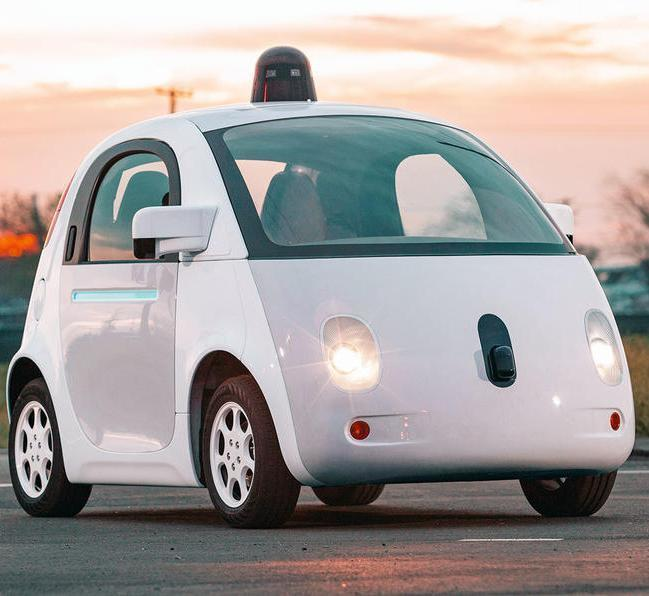
\includegraphics[height=3.00000cm]{imgs/googlecar.jpg}\label{fig:googlecar}}
\hspace*{\fill}

\caption{Exemples de robots mobiles dans la recherche}

\label{fig:mobilerecherche}

\end{figure}

L'industrie est également friande de robotique mobile, surtout grâce aux
Automatic Guided Vehicle (AGV, fig.~\ref{fig:agv}) qui permettent
d'améliorer la gestion et les performances d'un entrepôt, mais aussi
grâce à de plus modestes robots qui peuvent être vendus directement au
grand public, comme des aspirateurs (fig.~\ref{fig:roomba}) ou des
tondeuses.

\begin{figure}
\centering

\hspace*{\fill}
\subfloat[Transpalette robotique conçu par l'entreprise BA
Systèmes]{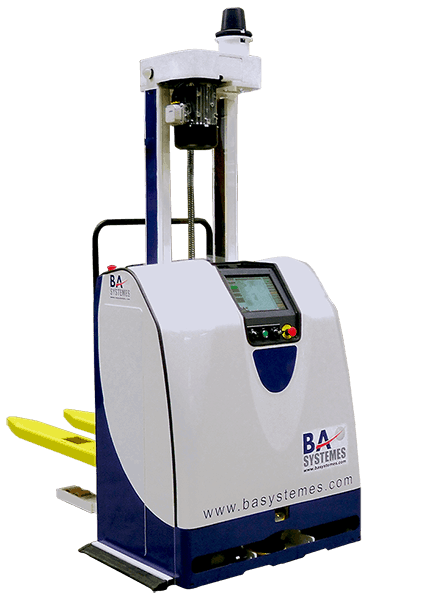
\includegraphics[height=5.00000cm]{imgs/agv.png}\label{fig:agv}}
\hfill%
\subfloat[Aspirateur robotique grand public
Roomba]{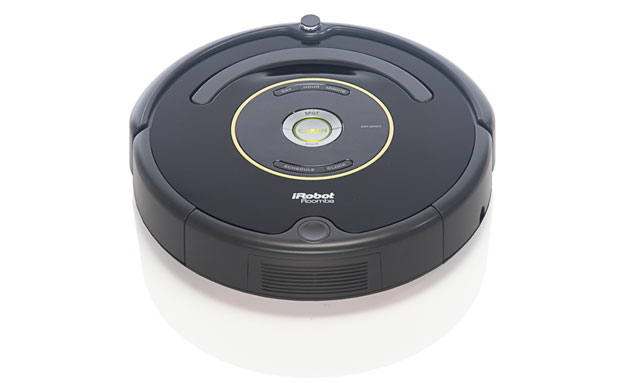
\includegraphics[height=5.00000cm]{imgs/roomba.jpg}\label{fig:roomba}}
\hspace*{\fill}

\caption{Exemples de robots mobiles dans l'industrie}

\label{fig:mobileindustrie}

\end{figure}

Enfin, la robotique mobile n'est pas non plus oubliée dans la
science-fiction, comme le montrent les exemples de robots mobiles bien
connus donnés dans la fig.~\ref{fig:mobilefiction}.

\begin{figure}
\centering

\hspace*{\fill}
\subfloat[Dalek, \emph{Dr Who},
1963]{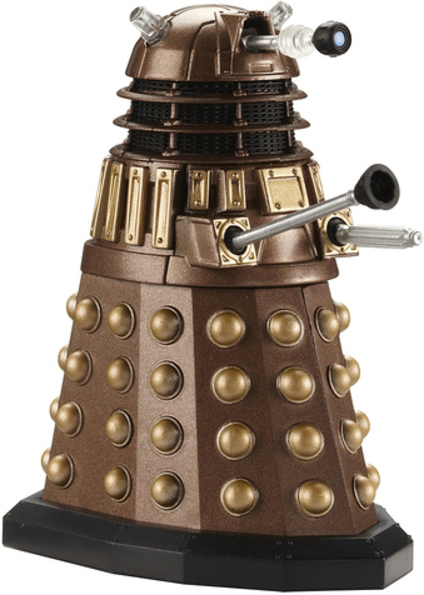
\includegraphics[height=4.00000cm]{imgs/dalek.jpg}\label{fig:dalek}}
\hfill%
\subfloat[R2-D2, \emph{Star Wars},
1977]{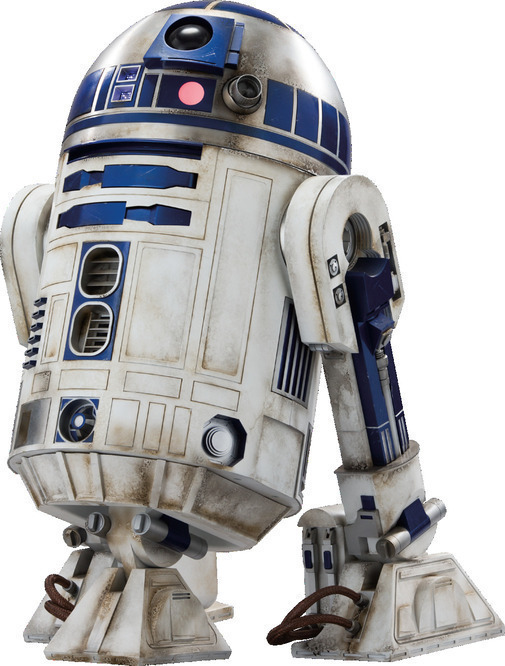
\includegraphics[height=4.00000cm]{imgs/r2d2.jpg}\label{fig:r2d2}}
\hfill%
\subfloat[Wall-E,
2008]{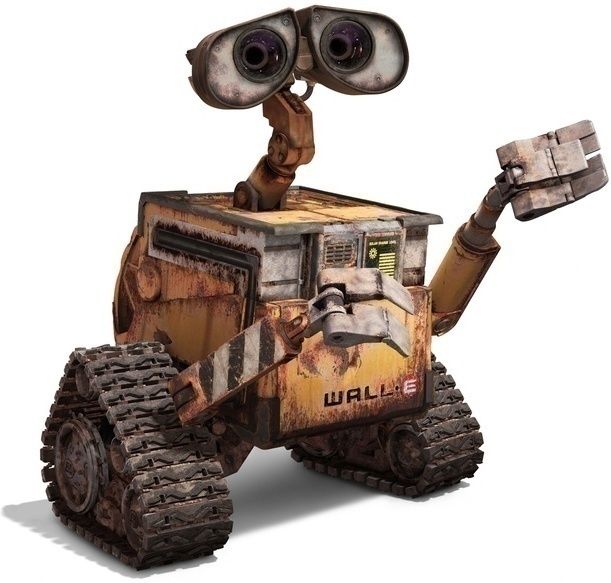
\includegraphics[height=4.00000cm]{imgs/wall-e.jpg}\label{fig:walle}}
\hspace*{\fill}

\caption{Exemples de robots mobiles dans la science-fiction}

\label{fig:mobilefiction}

\end{figure}

De nos jours, on trouve des applications à la robotique dans tous les
domaines de l'industrie, que ce soit pour la fabrication, la
manutention, ou le contrôle qualité. On la retrouve également dans un
nombre croissant d'autres secteurs, comme la médecine, l'agriculture,
les transports, ou encore le spatial.

En remplaçant ainsi l'homme dans un nombre croissant de tâches
difficiles, répétitives, fastidieuses, voire dangereuses, elle démontre
son impact sur la société ainsi que son intérêt économique.

De plus en plus, on retrouve également des robots dans notre quotidien,
comme le Roomba (fig.~\ref{fig:roomba}) présenté précédemment, ou encore
Pepper, un robot français de forme humanoïde (mais qui se déplace grâce
à trois roues omnidirectionnelles), qui peut servir d'hôte d'accueil, et
son petit frère Nao, utilisable comme plate-forme didactique.

\begin{figure}
\centering

\hspace*{\fill}
\subfloat[Nao, 2005,
58cm]{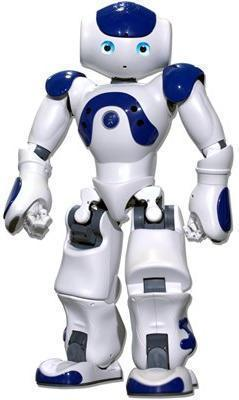
\includegraphics[height=7.00000cm]{imgs/nao.jpg}\label{fig:nao}}
\hfill%
\subfloat[Pepper, 2014,
121cm]{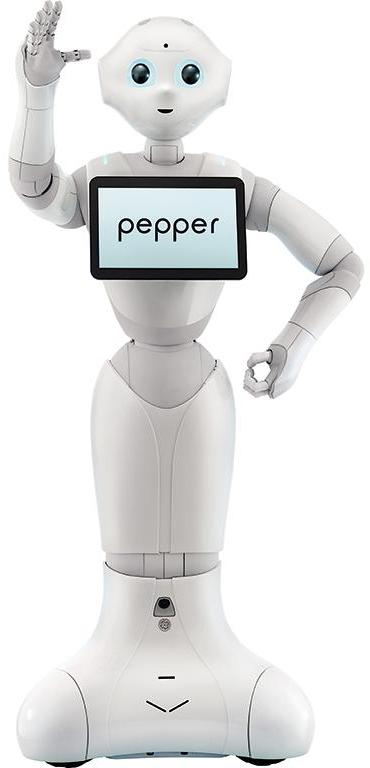
\includegraphics[height=7.00000cm]{imgs/pepper.jpg}\label{fig:pepper}}
\hspace*{\fill}

\caption{Robots d'Aldebaran Robotics prévus pour le grand public}

\label{fig:aldebaran}

\end{figure}

\section{Précautions d'usage}\label{sec:precautions}

Les applications possibles de la robotique sont innombrables.
Aujourd'hui, bon nombre d'entre elles n'attendent plus que du temps de
travail de roboticiens avant de pouvoir arriver dans nos vies, et faire
évoluer la société.

Cependant, cette évolution nécessite une réflexion. Comme le disait
Rabelais\,:

\begin{quote}
Science sans conscience n'est que ruine de l'âme. \par\raggedleft---
\emph{Pantagruel}, 1542
\end{quote}

Il appartient donc au scientifique de réfléchir avant d'agir.

Dans la majeure partie de cette thèse, nous parlons d'œuvres artistiques
et de science fondamentale, mais dans le chapitre \ref{sec:lemon}, nous
verrons un projet consistant à robotiser une tâche habituellement
effectuée par des êtres humains dans le but de recevoir une
rémunération.

Au XV\textsuperscript{ème} siècle, quand Gutenberg invente l'imprimerie,
les moines copistes perdent leur source de revenu, et sont remplacés par
des presses mécanisées. Les bénéfices pour l'humanité dans les décennies
et siècles à venir sont évidents.

Mais à plus court terme et à plus petite échelle, remplacer un être
humain par une machine n'est pas une mince affaire. Par exemple, on ne
veut pas voir des enfants travailler dans des usines de chaussures, mais
on ne veut pas non plus qu'ils meurent de faim à cause d'un manque
d'argent.

Pour l'instant, nous n'avons pas de solution miracle. Refuser la
robotisation pour protéger des emplois déjà existants ne résout que
temporellement certains problèmes pour en poser d'autres ensuite, comme
le montre le retard industriel que la France a pris sur l'Allemagne.

Il faut donc accompagner humainement au mieux les changements apportés
par ces nouvelles machines, voire repenser plus globalement la manière
dont sont distribuées les richesses.

Les chercheurs et industriels en robotique et en intelligence
artificielle sont au premier plan de ces réflexions, notamment avec la
création de groupes de travail internationnaux tels que « \emph{The IEEE
Global Initiative for Ethical Considerations in Artificial Intelligence
and Autonomous Systems}\footnote{\url{https://standards.ieee.org/develop/indconn/ec/autonomous_systems.html}}
» et le « \emph{future of life institute}\footnote{\url{https://futureoflife.org/ai-open-letter}}
».

À l'échelle locale, les universités et les laboratoires forment aussi
des comités d'éthique, et organisent également des opérations de
vulgarisation afin de communiquer avec le grand public et de lancer les
débats sur les enjeux qui apparaissent pour la société de demain.

\section{Plan}\label{sec:plan}

La robotique est intimement liée à la notion de mouvement. Le mouvement
peut notamment servir à la manipulation, la locomotion, ou à la
communication.

Dans cette thèse, nous nous intéresserons plus en détail à la
locomotion. La locomotion terrestre est généralement réalisée à l'aide
de roues ou de chenilles, ou par un système bipède, ou encore multipède.

Dans la partie \ref{sec:mobile}, nous étudierons la locomotion en
robotique mobile, c'est-à-dire sur des robots à roues, à travers deux
projets artistiques dans les chapitres \ref{sec:offroad} et
\ref{sec:transhumus} et un projet industriel dans le chapitre
\ref{sec:lemon}.

Puis dans la partie \ref{sec:humanoide} nous parlerons de robotique
humanoïde, et donc de locomotion bipède. Nous présenterons un cadre
logiciel destiné à concevoir un robot bipède, en optimisant
simultanément son design mécanique et son contrôle, dans le chapitre
\ref{sec:yoyoman}.

\section{Contributions}\label{sec:contributions}

Dans cette section, sous exposons les contributions de cette thèse.

En premier lieu, nous avons dirigé la réalisation technique de l'œuvre
\emph{transhumus} représentant la France lors de la Biennale de Venise
2015. Cette contribution est décrite dans le chapitre
\ref{sec:transhumus}, et a donné lieu aux publications suivantes:

\begin{itemize}
\tightlist
\item
  (Saurel, Taïx, et Laumond \protect\hyperlink{ref-transhumus}{2016})
\item
  Springer, à paraître
\end{itemize}

Ensuite, nous avons créé un cadre logiciel de codesign de marcheurs
bipèdes optimisant l'utilisation de leur dynamique passive intrinsèque.
Cette contribution est décrite dans le chapitre \ref{sec:yoyoman}, et a
donné lieu aux publications suivantes:

\begin{itemize}
\tightlist
\item
  (Saurel et al. \protect\hyperlink{ref-saurel16}{2016})
\item
  IROS, à paraître
\end{itemize}

Enfin, nous avons conçu une bibliothèque logicielle de planification de
trajectoire pour un robot autolaveur industriel. Cette contribution est
décrite dans le chapitre \ref{sec:lemon}.

\part{Étude de la robotique mobile}\label{sec:mobile}

\setcounter{figure}{0} \setcounter{table}{0} \setcounter{algorithm}{0}
\renewcommand{\thefigure}{\Roman{part}-\arabic{figure}}
\renewcommand{\thetable}{\Roman{part}-\arabic{table}}
\renewcommand{\thealgorithm}{\Roman{part}-\arabic{algorithm}}

\chapter*{Introduction~: Les robots à
roues}\label{introduction-les-robots-uxe0-roues}
\addcontentsline{toc}{chapter}{Introduction~: Les robots à roues}

Comme nous l'avons vu dans l'introduction générale, la robotique est
déjà bien présente dans notre quotidien.

Pour autant, la recherche en robotique est loin d'être terminée. Citons
par exemple les efforts humains et financiers actuellement fournis par
des entreprises comme Tesla, Google ou Uber, ainsi que de plus en plus
de constructeurs automobiles plus conventionnels, qui travaillent à
robotiser nos moyens de transports.

Afin de mieux comprendre comment la robotique permet à des systèmes de
se mouvoir, nous étudierons dans cette partie la locomotion en robotique
mobile, et plus particulièrement les robots à roues.

La roue est le premier et le plus simple des systèmes créés par l'homme
pour assurer des fonctions de déplacement. Elle est caractérisée par un
contact de roulement sans glissement, ce qui implique une contrainte
dite de non-holonomie sur les déplacements du robot qu'elle supporte.

Avec différents types de roues, positionnées suivant diverses
combinaisons, un robot peut se déplacer de différentes manières dans le
plan. Pour étudier ces différents types de robots, nous reprendrons la
classification de (Campion, Bastin, et Dandrea-Novel
\protect\hyperlink{ref-campion96}{1996}).

Cette classification repose sur l'étude des différents types de roues,
puis celle de la structure des modèles cinématiques et dynamiques de
robots constitués de ces roues. En introduisant les concepts de degré de
mobilité et de degré de dirigeabilité d'un robot mobile, elle démontre
que les robots mobiles peuvent être répartis en cinq classes.

Un robot mobile a donc un degré de mobilité \(\delta_m\), compris entre
1 et 3, correspondant au nombre de degrés de liberté pouvant être
directement actionnés. On lui attribue également un degré de
dirigeabilité \(\delta_s\), compris entre 0 et 2, indiquant le nombre de
roues pouvant être indépendamment réorientées pour diriger le robot.

La somme de ces deux nombres correspond au degré de manœuvrabilité du
robot \(\delta_M = \delta_m + \delta_s\), compris entre 2 et 3,
indiquant le nombre total de degrés de liberté dont il dispose dans son
mouvement dans le plan.

On a alors cinq classes de robots mobiles, notées
\((\delta_m, \delta_s)\), présentées dans la tbl.~\ref{tbl:campion}.

\hypertarget{tbl:campion}{}
\begin{longtable}[]{@{}llllll@{}}
\caption{\label{tbl:campion}Cinq classes de robots mobiles, d'après
(Campion, Bastin, et Dandrea-Novel
\protect\hyperlink{ref-campion96}{1996}) }\tabularnewline
\toprule
\(\delta_M\) & 3 & 2 & 3 & 2 & 3\tabularnewline
\midrule
\endfirsthead
\toprule
\(\delta_M\) & 3 & 2 & 3 & 2 & 3\tabularnewline
\midrule
\endhead
\(\delta_m\) & 3 & 2 & 2 & 1 & 1\tabularnewline
\(\delta_s\) & 0 & 0 & 1 & 1 & 2\tabularnewline
\bottomrule
\end{longtable}

Dans la suite de cette partie, nous donnerons dans le chapitre
\ref{sec:offroad} un exemple d'application pour des robots
différentiels, c'est-à-dire munis principalement de deux roues
motorisées, fixes, et sur le même axe (fig.~\ref{fig:differentiel}).
Puis, nous étudierons dans le chapitre \ref{sec:lemon}, un exemple de
robots munis de deux roues fixes et d'une tourelle, qui est une roue
dont le plan dans lequel elle tourne est orientable autour d'un axe
passant par son centre (fig.~\ref{fig:carlike}). Enfin, dans le chapitre
\ref{sec:transhumus}, nous terminerons cette partie avec un exemple de
robots munis de trois tourelles (fig.~\ref{fig:omni}).

\begin{figure}
\centering

\hspace*{\fill}
\subfloat[Différentiel (2,
0)]{\includegraphics[height=3.50000cm]{tikz/differentiel.pdf}\label{fig:differentiel}}
\hfill%
\subfloat[Car-like (1,
1)]{\includegraphics[height=3.50000cm]{tikz/carlike.pdf}\label{fig:carlike}}
\hfill%
\subfloat[Omnidirectionnel (1,
2)]{\includegraphics[height=3.50000cm]{tikz/omni.pdf}\label{fig:omni}}
\hspace*{\fill}

\caption{Trois classes de robots mobiles étudiés dans cette partie. Dans
ces schémas, les flèches représentent les degrés de liberté des roues,
parmi lesquels on retrouve ceux qui sont actionnés en rouge et gras.}

\label{fig:mobiles}

\end{figure}

Le robot omnidirectionnel ayant plus d'actionneurs que de degré de
manœuvrabilité, il est bien sûr nécessaire d'asservir certains de ces
actionneurs par rapport aux autres.

Ces robots sont respectivement de type \((2, 0)\), \((1, 1)\) et
\((1, 2)\). Nous verrons alors l'impact de la répartition des degrés de
mobilité et de dirigeabilité lorsque le degré de manœuvrabilité est
constant, puis l'impact de l'ajout d'un degré de dirigeabilité lorsqu'on
ne change pas le degré de mobilité sur la planification de mouvement
d'un robot.

\renewcommand{\thefigure}{\Alph{chapter}-\arabic{figure}}
\renewcommand{\thetable}{\Alph{chapter}-\arabic{table}}
\renewcommand{\thealgorithm}{\Alph{chapter}-\arabic{algorithm}}

\chapter{Robots mobiles différentiels}\label{sec:offroad}

Dans ce chapitre préambule, nous faisons le rapport d'un projet de
robotique réalisé juste avant le commencement de cette thèse. Il a
consisté à implémenter la génération de mouvements de robots mobiles
différentiels. Ces robots sont en réalité des pianos à queue, qui errent
dans un musée.

\section{\texorpdfstring{Introduction du projet \emph{off
road}}{Introduction du projet off road}}\label{introduction-du-projet-off-road}

\emph{Off road} est un projet robotique atypique, puisqu'il s'agit de la
réalisation d'une œuvre artistique.

L'artiste, l'exposition et l'œuvre sont présentés dans la suite de cette
section.

\subsection{Céleste
Boursier-Mougenot}\label{cuxe9leste-boursier-mougenot}

Céleste Boursier-Mougenot (fig.~\ref{fig:celeste}) est un artiste
plasticien, musicien et installationniste français.

\begin{figure}
\centering
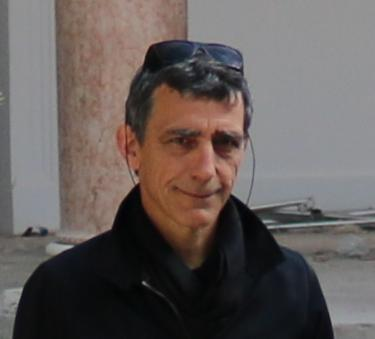
\includegraphics[height=3.00000cm]{imgs/celeste.jpg}
\caption{Céleste Boursier-Mougenot à la biennale de Venise en
2015}\label{fig:celeste}
\end{figure}

Il est notamment connu pour des œuvres comme \emph{from here to ear}
(fig.~\ref{fig:fromheretoear}), où le public voit un musée transformé en
volière abritant des dizaines de petits oiseaux, qui ont pour perchoir
des guitares électriques amplifiées disposées horizontalement pour les
accueillir.

C'est donc en se baladant que le visiteur joue de la musique, puisqu'il
fait s'envoler les oiseaux des cordes des guitares. L'artiste qualifie
alors sa musique de «~vivante~».

Parmi ses œuvres, on retrouve également \emph{clinamen}
(fig.~\ref{fig:clinamen}), dans laquelle des bols blancs flottent dans
une piscine circulaire bleutée, au gré d'un léger courant.

En s'entrechoquant, les bols en porcelaine forment une mélodie dont la
partition est finement réglée grâce au nombre et à la taille des bols,
ainsi que la force et la direction du courant.

On voit également sur la fig.~\ref{fig:clinamen} des bancs autour de la
piscine, invitant le visiteur à prendre le temps de s'assoir et à
profiter de l'œuvre, ce qui, paradoxalement, est plutôt rare dans un
musée. Cette idée, chère à l'artiste, se retrouve dans d'autres de ses
projets, comme \emph{zombiedrones} ou \emph{rêvolutions}.

\begin{figure}
\centering

\hspace*{\fill}
\subfloat[\emph{from here to ear}: des oiseaux se perchent sur une
guitare électrique
amplifiée]{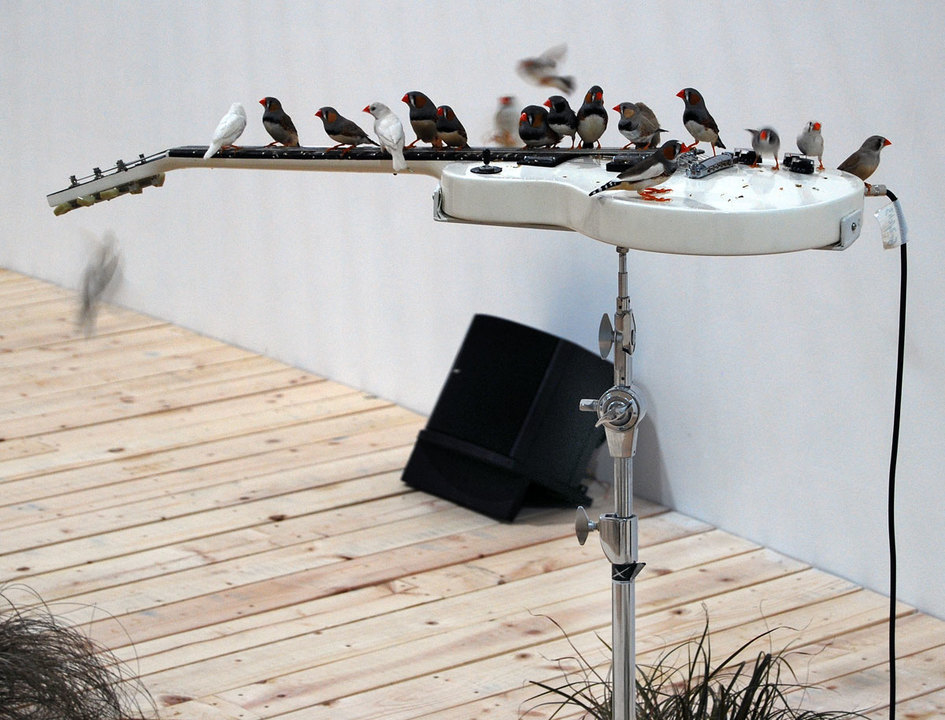
\includegraphics[height=4.00000cm]{imgs/from-here-to-ear.jpg}\label{fig:fromheretoear}}
\hfill%
\subfloat[\emph{clinamen}: des bols de porcelaine s'entrechoquent dans
une piscine suivant un courant
artificiel]{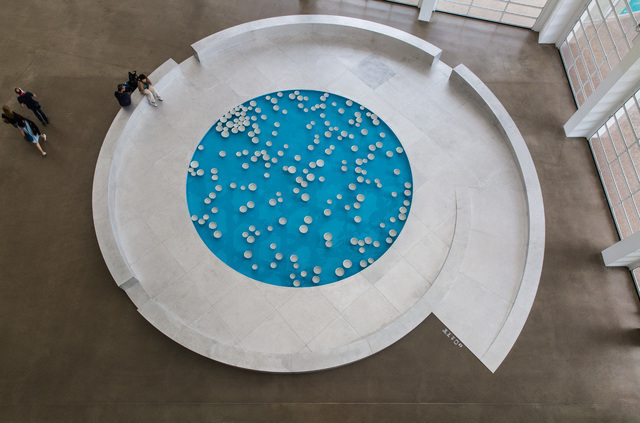
\includegraphics[height=4.00000cm]{imgs/clinamen.jpg}\label{fig:clinamen}}
\hspace*{\fill}

\caption{Œuvres classiques de Céleste Boursier-Mougenot.}

\label{fig:celeste-oeuvres}

\end{figure}

\subsection{Perturbations}\label{perturbations}

Du 31 janvier au 4 mai 2014, le musée des Abattoirs de Toulouse a
organisé l'exposition \emph{perturbations}
(fig.~\ref{fig:perturbations}), qui a principalement présenté cinq
œuvres de Céleste Boursier-Mougenot, dont deux inédites.

L'une de ces deux œuvres réalisées pour l'occasion s'intitulait
\emph{off road} (fig.~\ref{fig:offroad}), et consistait à doter de
locomotion trois pianos à queue.

\begin{figure}
\centering

\hspace*{\fill}
\subfloat[\emph{off road}: trois pianos à queue évoluent parmi le
public.]{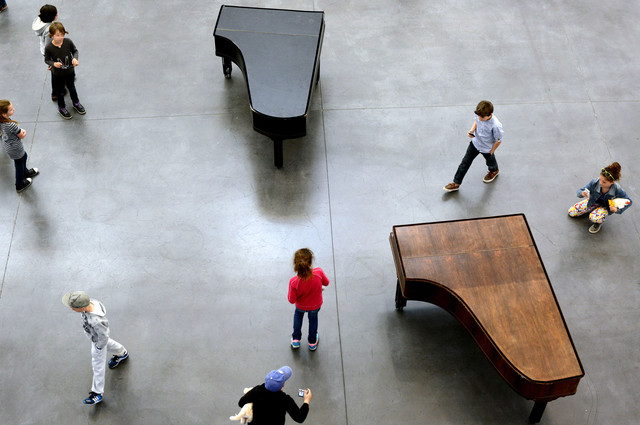
\includegraphics[width=1.00000\textwidth]{imgs/offroad.jpg}\label{fig:offroad}}
\hspace*{\fill}

\hspace*{\fill}
\subfloat[\emph{scanner}: un ballon sonde muni d'un micro erre grâce à
un ventilateur parmi des hauts-parleurs, créant des effets Larsen
modulés.]{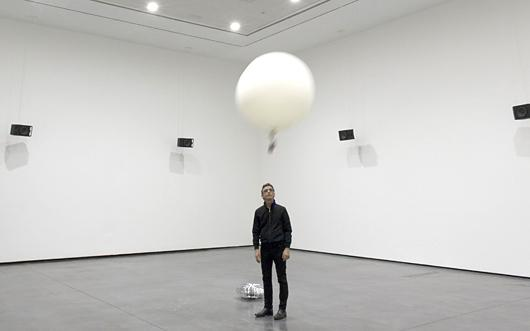
\includegraphics[height=3.50000cm]{imgs/scanner.jpg}} \hfill%
\subfloat[\emph{averses}: un détecteur de particules cosmiques déclenche
l'envoi d'une salve d'eau sur une batterie depuis le
plafond.]{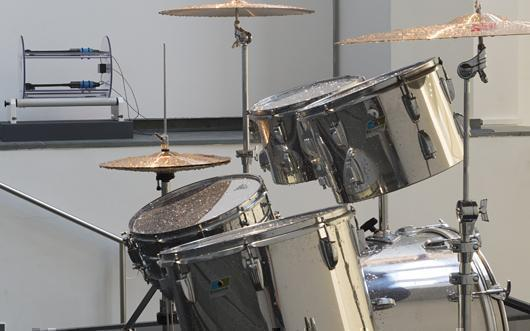
\includegraphics[height=3.50000cm]{imgs/averses.jpg}}
\hspace*{\fill}

\hspace*{\fill}
\subfloat[\emph{zombiedrone}: une télévision où chaque image est
soustraite à la précédente. La bande son est générée à partir de
l'image. Les visiteurs peuvent s'assoir et changer de
chaînes.]{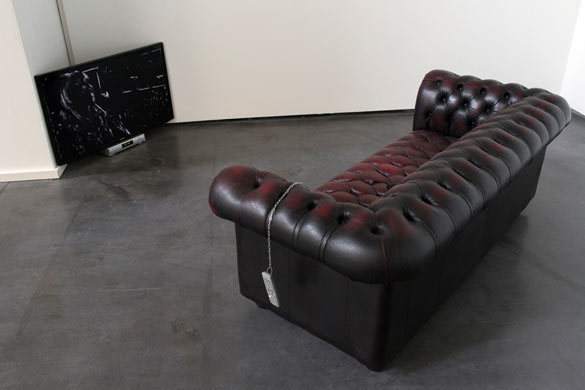
\includegraphics[height=3.50000cm]{imgs/zombiedrones.jpg}\label{fig:zombiedrone}}
\hfill%
\subfloat[\emph{U43}: un téléphone en bakélite noir de type U43 sonne
lorsque le mot «~fantôme~» apparaît sur Google
News.]{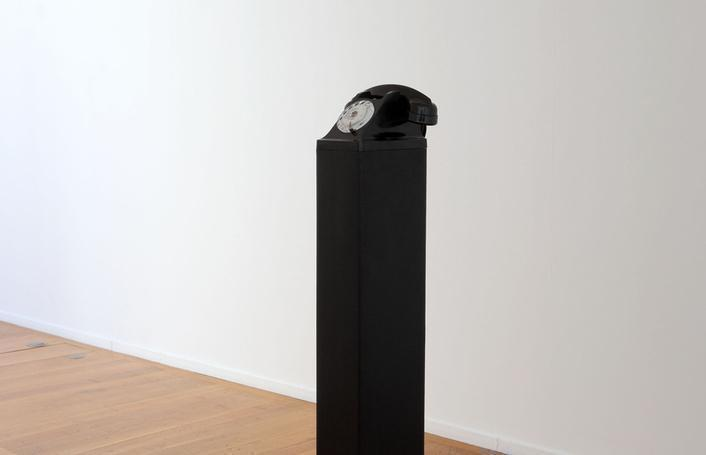
\includegraphics[height=3.50000cm]{imgs/u43.jpg}}
\hspace*{\fill}

\caption{Œuvres de Céleste Boursier-Mougenot lors de l'exposition
\emph{perturbations} du musée des Abattoirs de Toulouse en 2014.}

\label{fig:perturbations}

\end{figure}

\subsection{\texorpdfstring{\emph{Off road}}{Off road}}\label{off-road}

Dans cette œuvre, trois pianos à queue errent dans le musée.

Comme pour \emph{clinamen}, les pianos s'entrechoquent de temps en temps
ou heurtent les murs (généralement à faible vitesse), faisant ainsi
résonner leur table d'harmonie.

Et comme pour \emph{from here to ear}, le public fait partie de l'œuvre,
puisqu'il est invité, s'il l'ose, à errer parmi les pianos. Ce faisant,
il ignore que ces derniers peuvent décider de le fuir ou de le
poursuivre, comme nous les verrons par la suite,
sec.~\ref{sec:potentiels}.

Dans la suite de ce chapitre, nous détaillons la réalisation technique
de cette œuvre, financée par le musée des Abattoirs de Toulouse, dirigée
par l'artiste, et réalisée, en trois mois seulement, par Vincent
Angladon pour la gestion de la vision par ordinateur, Guilhem de Gramont
pour la mécanique, Korantin Auguste, Ken Hasselmann et moi-même pour la
robotique.

\section{Contrôle}\label{contruxf4le}

À son plus bas niveau, le contrôle du déplacement d'un robot nécessite à
minima des capteurs lui permettant de savoir quelle est sa position à un
instant donné, et des actionneurs lui permettant de se déplacer. Ces
deux composants doivent ensuite être reliés par un mécanisme de
décisionnel.

Dans cette section, nous verrons quelles solutions techniques ont été
mises en œuvre dans le cadre de ce projet pour ces besoins de perception
et d'action dans les secs.~\ref{sec:perception}, \ref{sec:action}, puis,
dans la section suivante, \ref{sec:planification}, quel mécanisme
décisionnel a été utilisé.

\subsection{Perception}\label{sec:perception}

Lorsqu'on évoque la perception, l'être humain pense à ses capteurs
internes qui constituent ses cinq sens. Pourtant, en robotique, il est
souvent plus aisé d'utiliser des capteurs qui ne sont pas embarqués dans
le robot.

Ainsi, pour de la géolocalisation de pianos à queue en intérieur pour
\emph{off road}, la plupart des solutions techniques que nous avons
envisagées, comprenant celle que nous avons retenue, consistaient à
équiper l'aire d'évolution des pianos plutôt que les pianos eux-mêmes.

En effet, dans une pièce connue, l'une des meilleures solutions pour
déterminer où un robot se situe et dans quelle orientation il est par
rapport à son environnement est d'utiliser un télémètre laser balayant
un plan horizontal. En ne gardant que les points les plus éloignés, on
trouve la position des murs, et détermine donc la position et
l'orientation du laser, et donc du robot, aux éventuelles symétries de
la salle près. Mais cette solution était largement en dehors de nos
moyens financiers.

Une seconde solution, au coût financier négligeable, et à la simplicité
et rapidité de mise en place appréciable, est l'odométrie. Elle consiste
à ajouter un capteur sur l'axe des roues afin de déterminer
incrémentalement la position à chaque instant. Cependant, la précision
de cette méthode s'amenuise au cours du temps, et n'est donc pas adaptée
à un système devant pouvoir fonctionner pendant une journée complète
sans intervention humaine. De plus, cette solution ne fonctionne pas si
la roue dérape ou saute. Dans notre cas, un choc entre deux pianos
semble suffisant important pour justifier que l'on n'utilise pas cette
technique.

Parmi les solutions externes de géolocalisation, il existe également la
triangulation et/ou trilatération à base d'ondes (dans le domaine
visible, auditif, WiFi, Bluetooth, \emph{etc.}). Cette solution, bien
qu'efficace (\emph{cf.} sec.~\ref{sec:transloc}), n'est pas simple à
mettre en place, et faute de temps et d'argent nous avons du
l'abandonner.

Notre choix s'est donc porté sur l'installation de caméras au plafond de
la pièce, et l'utilisation du traitement de ces images pour détecter la
position et l'orientation des trois pianos. Cette solution a entre
autres l'avantage d'être plutôt discrète, et également de nous permettre
de détecter les visiteurs si besoin (\emph{cf.}
sec.~\ref{sec:potentiels}).

La première étape est alors de fusionner les images des différentes
caméras, comme le montre la fig.~\ref{fig:merged}.

\begin{figure}
\centering
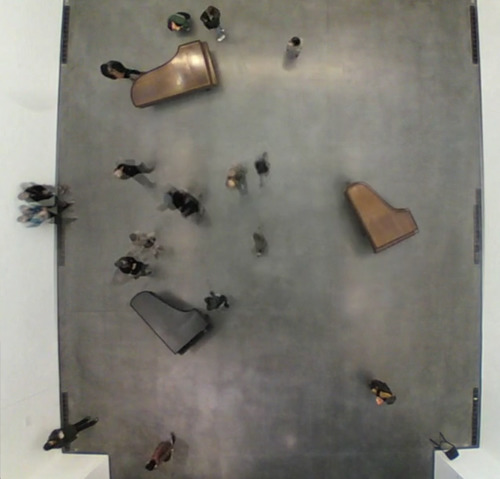
\includegraphics[height=9.00000cm]{imgs/merged.jpg}
\caption{Images des caméras au plafond superposées au niveau de
l'altitude des pianos.}\label{fig:merged}
\end{figure}

Malheureusement, la mise en œuvre de cette solution retenue ne s'est pas
révélée aussi simple que prévu. En effet, dans notre cas, la texture du
sol était similaire à celle des pianos, et le contraste entre leurs
teintes n'était pas suffisant, donc sous un éclairage uniforme, les
images présentaient un grain similaire pour les pianos et le sol, comme
en témoigne la fig.~\ref{fig:extraction}.

\begin{figure}
\centering
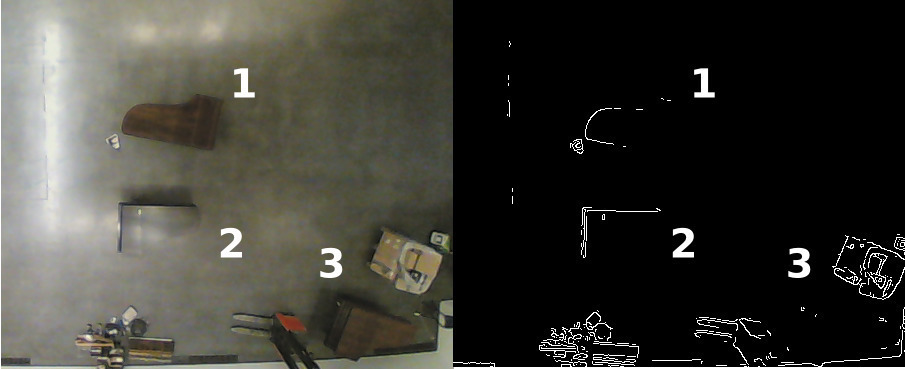
\includegraphics[height=5.00000cm]{imgs/pbvision.jpg}
\caption{Image des caméras à gauche, sortie de l'algorithme d'extraction
de contours pour cette image à droite. Les contours des machines sont
bien visibles, mais ceux des pianos sont estompés par endroits, y
compris pour l'œil humain.}\label{fig:extraction}
\end{figure}

Heureusement, en connaissant la position des pianos à un instant \(t\)
et leur vitesse approximative, il est possible de forcer l'algorithme
d'extraction des contours à chercher un contour particulier (connu) dans
un zone réduite à l'instant \(t + \delta t\).

En pratique, cela a fonctionné, mais a nécessité l'ajout d'une interface
utilisateur pour que les opérateurs (les guides et vigiles du musée)
positionnent correctement des masques sur les pianos le matin en
démarrant l'installation.

\subsection{Action}\label{sec:action}

Pour faire bouger ces pianos, deux moteurs ont été ajoutés et couplés
via une chaîne aux roues qui sont de part et d'autre du clavier. La
troisième roue, au bout de la queue, de type caster, n'est pas modifiée.
Le piano devient ainsi un robot mobile différentiel de type (2, 0)
(fig.~\ref{fig:piano}).

\begin{figure}
\centering
\includegraphics[height=6.00000cm]{tikz/piano.pdf}
\caption{Les pianos sont désormais des robots mobiles différentiel (2,
0)}\label{fig:piano}
\end{figure}

Sa vitesse linéaire \(v\) est donc proportionnelle à la moyenne des
vitesses des moteurs, et sa vitesse angulaire \(\omega\) est
proportionnelle à la différence des vitesses de ses moteurs, comme le
montre l'eq.~\ref{eq:differentiel}.

\begin{equation}
\begin{aligned}
v &= \cfrac{\omega_r + \omega_l}{2} \cdot r \\
\omega &= (\omega_r - \omega_l) \cdot r
\end{aligned}
\label{eq:differentiel}\end{equation}

où \(r\) est le rayon des roues du piano, et \(\omega_r\) et
\(\omega_l\) respectivement les vitesses appliquées aux roues droite et
gauche.

L'eq.~\ref{eq:differentiel} est vraie pour le point \(O\) du piano se
trouvant au milieu du clavier, donc tout point \(P\) du piano a une
vitesse \(\|v_P\| = v + \omega \cdot \| OP \|\).

On comprend donc que, lorsque le piano tourne, l'extrémité de sa queue
atteint rapidement une vitesse conséquente. Ce point n'est pas une
problématique à négliger lorsque la tête d'un enfant visiteur pourrait
se trouver au point d'intersection des trajectoires de deux pianos.

\section{Planification}\label{sec:planification}

Une fois que l'on connait à un instant donné la position
\((x, y, \alpha)\) d'un piano et qu'on est capable de le déplacer en
utilisant \((v, \omega)\), le robot est contrôlable~; mais il reste à
planifier, à plus haut niveau, ce que l'on veut que le robot fasse.

Naturellement, c'est à Céleste Boursier-Mougenot qu'il revient de
décider ce que les robots doivent faire. Mais bien sûr, c'était à nous,
roboticiens, d'implémenter techniquement le comportement choisi.

L'un des principaux challenges de ce projet a donc été d'arriver à nous
comprendre, artiste et roboticiens, sur les spécifications. Cela a donc
également été l'un des éléments les plus riches de cette collaboration.

Dans un premier temps, l'artiste nous a expliqué qu'il ne souhaitait pas
voir de mouvements «~robotiques~». Nous avons donc évité de donner aux
pianos des suites de consignes simple, comme avancer et reculer en ligne
droite, et tourner sur place, en suivant une machine à états classique.

Nous avons donc tenté d'implémenter des trajectoires plus «~douces~»,
telles que des splines. Cependant, des problèmes de nécessité de
prédiction ainsi que de deadlocks non triviaux se sont rapidement posés,
et les délais semblaient bien trop court pour que nous puissions
finaliser l'implémentation d'une telle solution à temps pour le
vernissage.

De plus, dans tous les cas, Céleste Boursier-Mougenot n'était pas
satisfait par le rendu artistique de nos premières itérations.

\subsection{Champs de potentiel}\label{sec:potentiels}

La solution aux problèmes évoqués ci-dessus a été d'utiliser la méthode
des champs de potentiel. Dans ce paradigme, on considère que l'aire
d'évolution des pianos est parsemée de potentiels \(P_i\) caractérisés
par une localisation, une norme \(\|P_i\|\), et un signe \(s_i\),
suivant si l'on désire un potentiel attractif ou un potentiel répulsif.

On calcule alors en un point \(p\) l'action de ce champ de potentiels
\(C(p)\) suivant l'eq.~\ref{eq:sumpot}.

\begin{equation} C(p) = \sum_i \cfrac{s_i \|P_i\|}{\mathrm{dist}(P_i, p) + 1} \label{eq:sumpot}\end{equation}

La fig.~\ref{fig:surface} montre un exemple de ce qu'il se passe si l'on
trace sur un graphe 3D l'allure de cette fonction dans l'aire
d'évolution des pianos. Il suffit alors d'imaginer une telle surface
comme un relief dans lequel le piano se baladerait en se déplaçant
suivant les pentes.

\begin{figure}
\centering
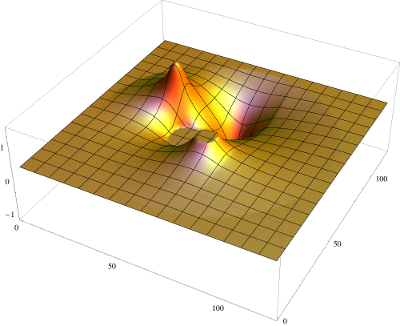
\includegraphics[width=1.00000\textwidth]{imgs/surface.png}
\caption{Champs de potentiels}\label{fig:surface}
\end{figure}

Il n'est donc plus nécessaire de prédire la trajectoire des pianos, et
en cas de deadlock il suffit d'ajouter un fort potentiel répulsif sur le
piano. De plus, le mouvement produit semble «~naturel~» et non
«~robotique~» pour un artiste, ce qui n'est pas une contrainte simple à
remplir en utilisant d'autres méthodes.

Par différences finies, on peut donc déterminer la forme de la «~pente~»
sur laquelle roule un piano, et donc ajuster sa vitesse en conséquence,
comme le montre l'eq.~\ref{eq:pots}.

\begin{equation} \begin{aligned}
v &= \cfrac{C(O + \varepsilon \vec{x}) - C(O - \varepsilon \vec{x})}{2\varepsilon} K_v \\
\omega &= \cfrac{C(O + \varepsilon \vec{y}) - C(O - \varepsilon \vec{y})}{2\varepsilon} K_{\omega_{}}
\end{aligned} \label{eq:pots}\end{equation}

Dans notre cas, nous avons considéré les murs et d'autres zones
interdites comme des potentiels répulsifs constants. En jouant sur la
norme du potentiel des murs, on peut modifier la fréquence à laquelle
les pianos vont s'y cogner. On peut alors contenter à la fois l'artiste
qui désire que cela puisse arriver, et l'équipe du musée qui doit
maintenir les murs dans un état correct\footnote{Un rideau de scène de
  8.30 × 13.25m réalisé par Pablo Picasso se trouve en permanence
  derrière l'une de ces cloisons. On comprendra donc que l'équipe du
  musée tienne à ce que la cloison ne s'effondre pas.}.

Ensuite, les pianos sont vus les uns par les autres comme des
potentiels, tantôt attractifs tantôt répulsifs, jusqu'à ce que l'on
détecte un choc. À ce moment-là, les pianos deviennent de forts
potentiels répulsifs l'un pour l'autre pour une durée limitée.

Enfin, selon les circonstances, le système de planification peut repérer
un visiteur (toujours grâce aux caméras présentes au plafond), et le
considérer comme un potentiel attractif ou répulsif.

\subsection{Entrée du système}\label{entruxe9e-du-systuxe8me}

Comme nous l'avons vu dans la sec.~\ref{sec:potentiels}, il suffit
d'ajouter des potentiels pour que les pianos bougent. Cependant, Céleste
Boursier-Mougenot souhaite que le comportement de ses œuvres ne soit ni
prédictibles, ni dictés par un générateur de nombres aléatoires.

Ainsi, dans les œuvres décrites dans la fig.~\ref{fig:perturbations},
des éléments extérieurs comme les particules cosmiques, les résultats en
temps réel de Google News ou encore les chaînes de télévision sont
introduits et dirigent l'expérience du visiteur.

Dans \emph{off road}, l'artiste a choisi d'utiliser le vent. Nous avons
donc installé une girouette et un anémomètre sur un mur extérieur du
musée, de sorte qu'ils soient visibles à travers des fenêtres lorsqu'on
est à côté de l'œuvre.

La vitesse du vent, son accélération, et sa direction sont donc dans
cette œuvre les principaux facteurs qui créent des potentiels, soit
directement, soit indirectement en désignant un visiteur. Celui-ci peut
ainsi, sans le savoir, faire partie de la performance.

\section{Architecture Matérielle et
Logicielle}\label{architecture-matuxe9rielle-et-logicielle}

Dans un premier temps, l'artiste voulait que les pianos soient «~maîtres
d'eux-mêmes~», et donc que nous embarquions tous nos algorithmes dans de
petits ordinateurs à leur bord.

Sur le plan théorique, cela ne change pas grand-chose. Les batteries de
voitures déjà embarquées sur les pianos suffisent largement à alimenter
en plus un mini ordinateur de type Raspberry Pi ou NUC/Brix suivant la
puissance de calcul requise.

Cependant, en termes de complexité de déploiement, le coût en temps
était trop élevé. De plus, les choix présentés en
sec.~\ref{sec:perception} imposaient la présence d'une interface
utilisateur dans le musée.

Nous avons donc utilisé une architecture centralisée, où un ordinateur
de bureau, muni d'un écran, d'un clavier et d'une souris, restait à
disposition de l'équipe du musée, et servait à orchestrer les
déplacements des pianos.

La fig.~\ref{fig:overview} explique l'architecture matérielle utilisée
pour cette œuvre.

\begin{figure}
\centering
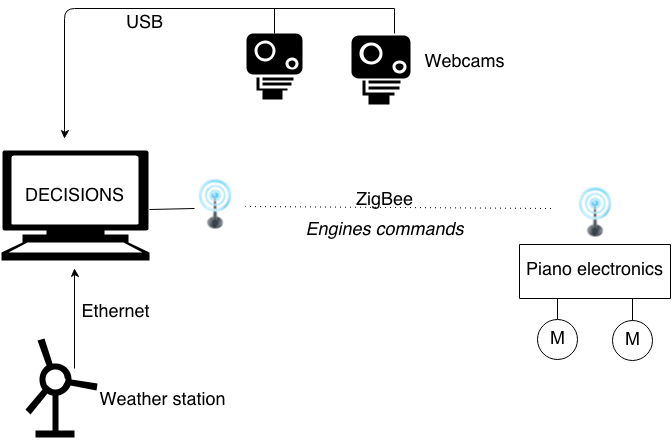
\includegraphics[width=1.00000\textwidth]{imgs/overview.png}
\caption{Architecture matérielle de l'œuvre \emph{off
road}.}\label{fig:overview}
\end{figure}

On y retrouve deux caméras décrites à la sec.~\ref{sec:perception},
attachées au plafond, reliées par USB directement sur l'ordinateur
principal.

Un module XBEE est également connecté à cet ordinateur, et envoie des
ordres aux pianos grâce au protocole ZigBee.

Sur les pianos, on retrouve ces différents composants:

\begin{itemize}
\tightlist
\item
  Une batterie de voiture 12V 120Ah;
\item
  Deux moteurs;
\item
  Un module XBEE pour recevoir les ordres de l'ordinateur principal
  (fig.~\ref{fig:xbee});
\item
  Un accéléromètre pour détecter les chocs;
\item
  Un capteur de courant par sécurité;
\item
  Une carte de contrôle moteur 60A (fig.~\ref{fig:sabertooth});
\item
  Un Arduino (fig.~\ref{fig:arduino}) qui implémente
  l'eq.~\ref{eq:differentiel}, gère les autres composants électroniques,
  et remonte des données sur l'état courant à l'ordinateur principal;
\item
  Un «~shield~» Arduino sur mesure pour connecter tous ces composants
  électroniques (fig.~\ref{fig:shield}).
\end{itemize}

Enfin, la station météo (fig.~\ref{fig:meteo}) est connectée à un
Arduino qui interprète les données analogiques, et les envoie à une
Raspberry Pi (fig.~\ref{fig:raspi}) en USB, qui à son tour les transmet
à l'ordinateur principal en ethernet grâce à la librairie ZeroMQ.

Cette solution a été choisie puisque d'une part nous avions déjà tous
les composants nécessaires (et nous n'avions que très peu de temps pour
des commandes de matériel supplémentaire), et d'autre part il y a besoin
de plusieurs dizaines de mètres de câbles. L'ethernet est donc l'une des
seules liaisons physiques viables.

Tous ces composants sont illustrés sur la
fig.~\ref{fig:offroadcomponents}.

\begin{figure}
\centering

\hspace*{\fill}
\subfloat[Raspberry Pi, un ordinateur avec un processeur ARM de la
taille d'une carte de
crédit.]{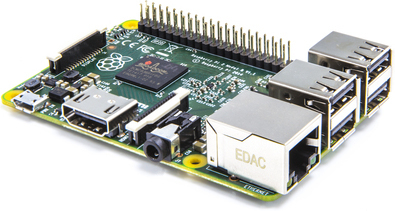
\includegraphics[width=0.55000\textwidth]{imgs/raspi.jpg}\label{fig:raspi}}
\hfill%
\subfloat[Arduino, un microcontrolleur simple à
utiliser.]{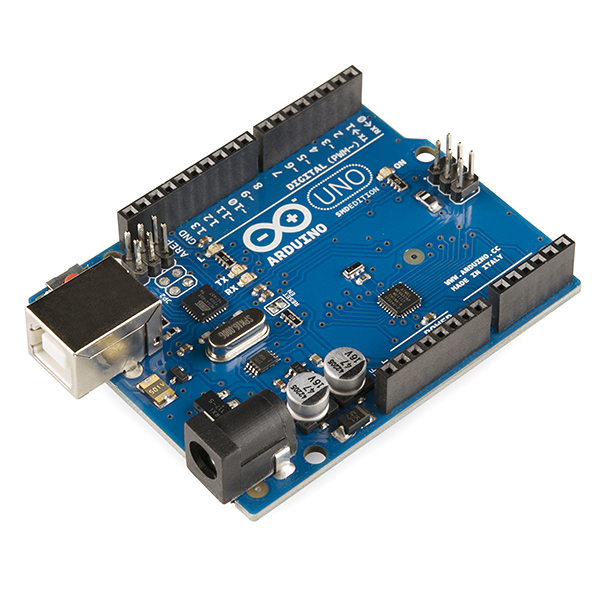
\includegraphics[width=0.35000\textwidth]{imgs/arduino.jpg}\label{fig:arduino}}
\hspace*{\fill}

\hspace*{\fill}
\subfloat[Module XBEE, pour transmettre des données sans fil selon le
protocole
ZigBee.]{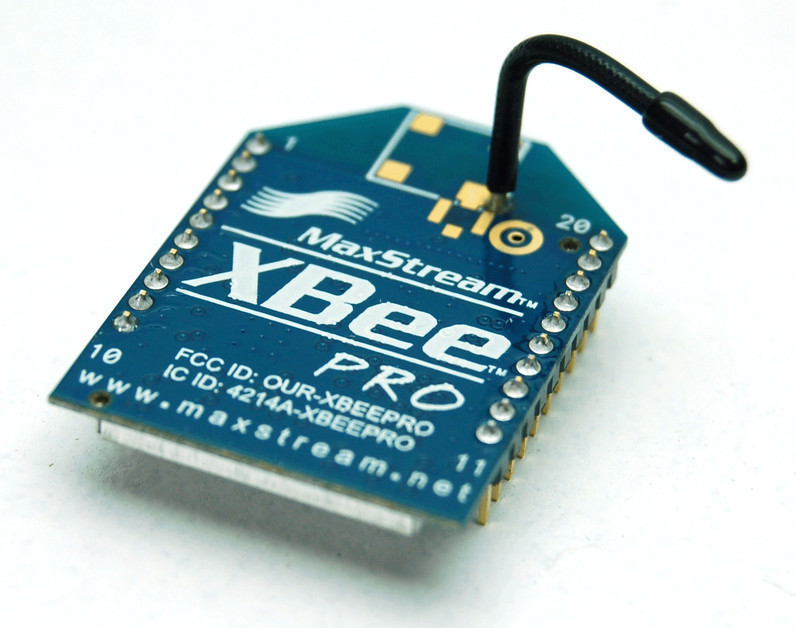
\includegraphics[width=0.45000\textwidth]{imgs/xbee.jpg}\label{fig:xbee}}
\hfill%
\subfloat[Carte de contrôle
moteurs.]{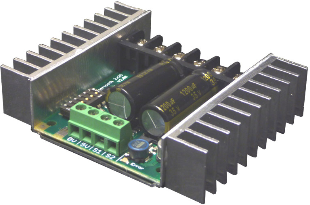
\includegraphics[width=0.45000\textwidth]{imgs/sabertooth.png}\label{fig:sabertooth}}
\hspace*{\fill}

\hspace*{\fill}
\subfloat[Layout du shield Arduino conçu sur mesure. L'effet miroir est
inhérent à la technologie utilisée pour graver le circuit
imprimé.]{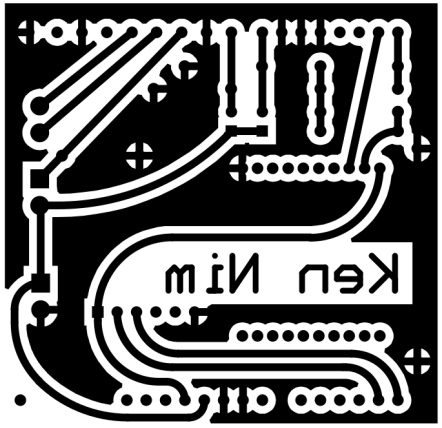
\includegraphics[height=5.00000cm]{imgs/kennim.png}\label{fig:shield}}
\hfill%
\subfloat[Schéma électrique de la girouette et de l'anémomètre
utilisés.]{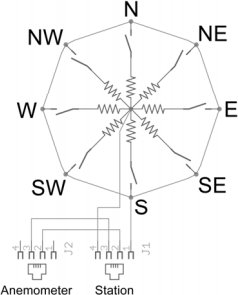
\includegraphics[height=5.00000cm]{imgs/analog.png}\label{fig:meteo}}
\hspace*{\fill}

\caption{Composants matériels utilisés pour \emph{off road}.}

\label{fig:offroadcomponents}

\end{figure}

Une manette de XBOX était également fournie et branchée sur l'ordinateur
principal, afin de pouvoir déplacer manuellement les pianos.

Du point de vue logiciel, tous nos développements ont été effectués en C
pour les microcontrolleurs et en Python pour le reste.

Le protocole de communication entre les arduinos des pianos et
l'ordinateur principal a été créé sur mesure.

\section{Résultats}\label{ruxe9sultats}

Avec seulement trois mois pour la réalisation complète du projet, il n'y
a pas eu de temps pour faire des tests en conditions réelles. L'œuvre a
été achevée le jour du vernissage de l'exposition, le 29 janvier 2014,
et a tenu jusqu'à sa fin, le 4 mai suivant.

Le seul problème technique qui s'est posé à quelques reprises était une
perte de masque de la vision, généralement due à des changements
d'éclairage (\emph{eg.} grillage d'une ampoule dans la salle).

Malgré la présence de bouton d'arrêt d'urgence, et de nos tentatives
d'explications techniques à l'équipe du musée, cela a quand même causé
la destruction partielle de l'un des pianos, lorsqu'il a percuté un
escalier à pleine vitesse.

\subsection{Qualité du mouvement}\label{qualituxe9-du-mouvement}

Il est difficile de décrire le mouvement final à l'écrit, mais plusieurs
vidéos\footnote{\url{http://dai.ly/x1di66l?start=314}}\footnote{\url{https://vimeo.com/87218362}}\footnote{\url{https://youtu.be/cF4aS3LsHcg}}
ont été réalisées et montrent plus précisément le résultat final.

\subsection{Suites du projet}\label{suites-du-projet}

Nous avons par la suite été contactés par une équipe d'Airbus qui avait
initialement jugé le projet impossible à réaliser compte tenu du budget
et des délais, afin de leur présenter nos méthodes et nos solutions
techniques.

Jean-Paul Laumond, intrigué par cette application inattendue du problème
classique du déménageur de pianos (Schwartz, Sharir, et Hopcroft
\protect\hyperlink{ref-schwartz87}{1987}), ainsi que par notre
utilisation de la méthode des champs de potentiel, a également voulu
nous rencontrer suite à ce vernissage. Ceci a donc participé à la
réalisation de cette Thèse.

\chapter{Robots mobiles à tourelle}\label{sec:lemon}

Dans ce chapitre, nous faisons le rapport d'un projet de robotique
réalisé lors de cette thèse en coopération avec l'entreprise BA
Systèmes.

\section{Introduction du projet
LEMON}\label{introduction-du-projet-lemon}

Le projet LEMON, bien plus prosaïque que les autres projets de cette
partie, porte sur la conception d'un robot qui remplacerait une
autolaveuse autoportée et son opérateur, dans des endroits tels qu'une
station de métro ou un hôpital.

Le prototype d'un tel robot a été réalisé par la société BA Systèmes, et
un accord a été conclu avec le LAAS-CNRS pour que nous concevions
l'algorithme de planification de trajectoire.

Ce projet a grandement bénéficié de l'expertise de Florent Lamiraux en
planification de trajectoires pour la robotique mobile, ainsi que de la
trousse de développement logiciel libre HPP\footnote{Humanoid Path
  Planner}, développée au sein de l'équipe Gepetto (Mirabel et al.
\protect\hyperlink{ref-hpp}{2016}).

Dans la suite de ce chapitre, nous verrons en premier lieu comment nous
cartographions une zone afin de faciliter la planification de
trajectoire dans la sec.~\ref{sec:carto}.

Le robot doit ensuite utiliser une brosse latérale rétractable afin de
nettoyer les bords des murs, ce qui est détaillé dans la
sec.~\ref{sec:bordures}. Après cela, le robot doit nettoyer les aires
libres d'obstacles grâce à sa brosse principale, comme nous le verrons
dans la sec.~\ref{sec:surfaces}.

Enfin, nous expliquerons comment nous relions au mieux toutes ces
portions de trajectoires dans la sec.~\ref{sec:trajectoirefinale}, puis
quelles optimisations nous avons ajouté dans la
sec.~\ref{sec:optimisation}.

Pour conclure, nous exposerons nos résultats et leurs limitations dans
la sec.~\ref{sec:lemonres} et les perspectives dans la
sec.~\ref{sec:lemonfutur}.

\section{Création de la carte}\label{sec:carto}

Dans cette section, nous partons d'un plan généré par les capteurs laser
du robot, constitué d'une liste d'obstacles.

Afin de réaliser des tests de performances dans un maximum de cas, ce
plan peut provenir de différentes sources\,:

\begin{itemize}
\tightlist
\item
  un fichier texte généré par le prototype de BA Système composé de deux
  nombres par lignes indiquant les coordonnées de chaque point obstacle
  trouvé par les lasers;
\item
  une image (par exemple un plan d'architecte) et une échelle;
\item
  en utilisant directement l'API de la librairie implémentée pour
  l'occasion, par exemple dans un contexte de production sur le robot.
\end{itemize}

L'objectif est d'extraire la position des murs de ce nuage de point,
afin de générer des trajectoires de balayage des bords de ces murs. On a
aussi besoin de pouvoir savoir où le robot peut passer ou non.

Pour cela, nous créons une classe \texttt{Bitmap} pour discrétiser la
zone d'évolution. Ses bords sont ceux d'un rectangle dont la largeur, la
longueur et l'orientation sont calculées automatiquement pour englober
la surface à nettoyer et limiter la consommation en mémoire, et donc
ainsi optimiser la vitesse d'exécution des algorithmes suivants.

Cette classe \texttt{Bitmap} est composée de \texttt{Pixels}, qui
peuvent avoir plusieurs étiquettes:

\begin{itemize}
\tightlist
\item
  \texttt{OBSTACLE} si au moins un point obstacle est à l'intérieur;
\item
  \texttt{FREE} sinon;
\item
  \texttt{BOUNDARY} si c'est un \texttt{FREE} directement à côté d'un
  \texttt{OBSTACLE};
\item
  \texttt{REACHABLE} si c'est un \texttt{FREE} accessible au robot;
\item
  \texttt{CLEANED} s'il est sur le chemin de balayage final.
\end{itemize}

D'autres \texttt{OBSTACLES} peuvent être ajoutés par un utilisateur pour
définir des zones interdites circulaires ou polygonales. On en ajoute
également tout autour de l'aire définie par le \texttt{Bitmap}.

Les zones \texttt{REACHABLE} sont calculées à partir de la position de
départ du robot, ainsi que de ses dimensions physiques.

Une zone de tests a été réalisée dans les locaux de BA Systèmes, et nous
en avons crée une carte (fig.~\ref{fig:carte}).

Sur cette image, les \texttt{Pixels} en rouge contiennent des
\texttt{OBSTACLES}, ceux en bleu sont des \texttt{BOUNDARY}, et ceux en
verts représentent les \texttt{FREE} dont l'intensité varie avec la
distance aux \texttt{Pixels} de type \texttt{OBSTACLE}. Cette distance
nous permet de savoir où le robot peut passer ou non.

\begin{figure}
\centering
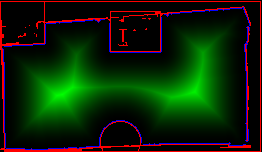
\includegraphics[width=1.00000\textwidth]{imgs/carte.png}
\caption{Exemple de carte créée avec la classe
\texttt{Bitmap}.}\label{fig:carte}
\end{figure}

\section{Trajectoires de nettoyage des bordures}\label{sec:bordures}

Dans un premier temps, une fois que la carte de la zone est disponible,
nous souhaitons utiliser la brosse latérale rétractable du robot afin de
balayer le long des murs.

Dans cette section, nous expliquons comment nous détectons les segments
de droites et les arcs de cercle dans cette carte, afin de donner des
consignes simples au robot.

L'objectif est de fournir la première partie de la \texttt{Roadmap}
destinée au robot. Cette \texttt{Roadmap} sera dans un premier temps
composée d'une liste de segments définis par des paires \((q_s, q_e)\)
indiquant les positions initiales et finales nécessaires pour nettoyer
chaque bordure.

\subsection{Détection des segments de
droites}\label{sec:borduresdroites}

L'obstacle le plus courant est un mur rectiligne. Il nous parait donc
logique de commencer par chercher ce type d'obstacle. Pour trouver la
liste des \texttt{Pixels} de type \texttt{BOUNDARY} qui sont sur des
segments de droite, nous utilisons une transformée de Hough (Duda et
Hart \protect\hyperlink{ref-hough}{1972}), décrite dans
l'alg.~\ref{alg:hough}.

\begin{algorithm}
\caption{Transformée de Hough}
\label{alg:hough}
\begin{algorithmic}[1]

\Procedure{HoughTransform}{$\texttt{BOUNDARY}, N_\rho, N_\theta$}

\State $\mathcal{H} \gets 0_{N_\rho, N_\theta}$
\Comment{Initialisation de la matrice $\mathcal{H}$}
\State $\bm{\bar\theta} \gets \operatorname{linspace}(-\pi, \pi, N_\theta)$
\Commente{et des ensembles discretisés}
\State $\bm{\bar\rho} \gets \operatorname{linspace}(0, \sqrt{x_{max}^2+y_{max}^2}, N_\rho)$
\Commente{de coordonées polaires.}

\For{$(x, y) \in \texttt{BOUNDARY}$}
\For{$\theta \in \bm{\bar\theta}$}
\State $\rho \gets \arg\min\limits_{\rho \in \bm{\bar\rho}}(|x \cos(\theta) + y \sin(\theta) - \rho|)$
\State $\mathcal{H}_{\rho,\theta} \gets \mathcal{H}_{\rho,\theta} + 1$
\Comment{Incrémentation du coefficient obtenu.}
\EndFor
\EndFor

\State \textbf{return} $\mathcal{H}$
\EndProcedure

\end{algorithmic}
\end{algorithm}

Cette transformée consiste à créer une matrice dite de Hough,
\(\mathcal{H}\), dont les dimensions sont la discretisation souhaitée de
l'espace en coordonnées polaires \((\rho, \theta)\):
(\(N_\rho, N_\theta\)).

Ensuite, chaque point \((x, y)\) de l'ensemble \texttt{BOUNDARY}
«~vote~» pour la liste des droites \((\rho, \theta)\) dont il pourrait
faire partie.

Le résultat de cette transformée de Hough est alors la matrice de Hough
\(\mathcal{H}\), dont les coefficients les plus importants indiquent les
paramètres des droites les plus probables.

Afin de détecter les trajectoires qui balaient les bordures, on utilise
ensuite le cadre logiciel HPP pour simuler un passage de ce robot
suivant les droites fournies par la matrice de Hough dans les deux sens.

On garde alors les portions de ces trajectoires qui nettoient
effectivement des \texttt{Pixels} de type \texttt{BOUNDARY} et qui ne
présentent pas de collisions entre le robot et son environnement.

Enfin, on enlève les \texttt{Pixels} ainsi nettoyés de l'ensemble de
ceux de type \texttt{BOUNDARY} et on recommence autant de fois que
nécessaire.

L'extraction complète de ces trajectoires est explicitée dans
l'alg.~\ref{alg:segments}, et dans l'annexe~\ref{sec:annlemon}.

\begin{algorithm}
\caption{Détection des segments de droite à balayer}
\label{alg:segments}
\begin{algorithmic}[1]

\While{$\texttt{BOUNDARY} \neq \varnothing$}
\For{$(\rho, \theta) \in \arg\max(\Call{HoughTransform}{\texttt{BOUNDARY}, N_\rho, N_\theta})$}
\State\Call{followLine}{$\rho, \theta, +1$}
\State\Call{followLine}{$\rho, \theta, -1$}
\EndFor
\EndWhile

\Procedure{followLine}{$\rho, \theta, \sigma$}
\State $start \gets false$
\For{$q \in \Call{line}{\rho, \theta, \sigma}$}
\Comment{\parbox[c]{.45\linewidth}{$\sigma$ est le sens de parcours à suivre. {\sc line} est explicité en
annexe~\ref{sec:annlemon}.}}
\State $valid \gets \Call{chkPos}{q}$
\Comment{\parbox[c]{.55\linewidth}{Place le robot pour que la brosse soit positionnée en $q$ et vérifie les
collisions et qu’on nettoie bien des \texttt{BOUNDARY}}}
\If{$valid \Ands \overline{start}$}
\State $start \gets true$
\State $q_s \gets q$
\Comment{Début d’une trajectoire}
\ElsIf{$start \Ands \overline{valid}$}
\State $start \gets false$
\State $\Call{addLane}{q_s, q}$
\Comment{\parbox[c]{.5\linewidth}{Ajoute la trajectoire à la \texttt{Roadmap} et supprime les \texttt{BOUNDARY}
nettoyées}}
\EndIf
\EndFor
\EndProcedure

\end{algorithmic}
\end{algorithm}

\subsection{Détection des arcs de cercle}\label{sec:bordurescourbes}

Les environnements dans lesquels le robot LEMON est destiné à évoluer
peuvent aussi comporter des obstacles circulaires. Par exemple, une
station de métro peut suivre une voie ferrée courbée. On peut également
voir des piliers ronds.

Ces arcs de cercle pourraient dans certains cas être approximés par des
suites de segments, mais en pratique les résultats n'étaient pas
satisfaisants. Nous avons donc ajouté à l'algorithme présenté dans la
section précédente une phase de transformée de Hough circulaire.

Un opérateur doit alors entrer la liste des rayons de cercles qui sont
présent dans un environnement, et, pour chacun de ces rayons, nous
construisons une matrice de Hough dont les coefficients correspondent
aux coordonnées \((x, y)\) du centre d'un cercle d'un tel rayon à la
place des coordonnées \((\rho, \theta)\) d'une droite.

\section{Trajectoires de nettoyage des surfaces}\label{sec:surfaces}

Dans cette section, nous présentons la stratégie de balayage des
surfaces retenue. Ce balayage de surface intervient après le balayage
des bordures.

De la première transformée de Hough pour la détections des segments de
droites (\emph{cf.} sec.~\ref{sec:borduresdroites}), nous extrayons la
droite de la transformée de Hough ayant le plus de \texttt{Pixels}.

Depuis cette droite principale, nous traçons des segments parallèles qui
couvrent la surface, tout en prenant toujours soin d'éviter les
collisions avec l'environnement grâce à la procédure \textsc{followLine}
décrite dans l'alg.~\ref{alg:segments}.

Pour chaque segment ainsi généré, nous ajoutons deux trajectoires dites
«~symétriques~» à la \texttt{Roadmap}, qui correspondent aux deux sens
de parcours du segment par la brosse principale du robot.

Il suffit alors que l'une des deux trajectoires de la paire soit suivie
par le robot pour considérer que la paire est traitée.

\section{Génération de la trajectoire
finale}\label{sec:trajectoirefinale}

Une fois que les trajectoires de balayage des bordures droites
(sec.~\ref{sec:borduresdroites}) et courbes
(sec.~\ref{sec:bordurescourbes}) ainsi que les trajectoires symétriques
de nettoyage des surfaces (sec.~\ref{sec:surfaces}) sont entrées dans la
\texttt{Roadmap} sous forme de paires de configuration \((q_s, q_e)\),
il reste à générer la trajectoire finale.

Pour cela, il faut commencer par déterminer l'ordre de parcours des
trajectoires de balayage des bordures, puis celui des trajectoires de
nettoyage des surfaces. La trajectoire finale consiste alors à relier la
suite de configurations obtenue par des trajectoires dites de «~Reeds
and Shepp~» (Reeds et Shepp \protect\hyperlink{ref-reedsshepp}{1990}).

Dans le but de déterminer l'ordre de parcours des trajectoires, nous
avons utilisé un algorithme glouton. Ainsi, à partir de la position
initiale du robot, nous recherchons la configuration de départ de la
trajectoire de suivi balayage des bordures la plus proche, au sens de la
distance de Reeds and Shepp, et suivant la méthode de tir aléatoire
RRT-Connect (Kuffner et LaValle \protect\hyperlink{ref-rrt}{2000}).

Ensuite, nous repartons de la configuration finale associée, et
recommençons l'opération jusqu'à ce que toutes les trajectoires de
balayage des bordures soient effectuées. Le même procédé est alors
répété à partir de la configuration finale de la dernière trajectoire de
balayage des bordures pour les trajectoires de nettoyage des surfaces.

Les principaux algorithmes de cette section, qui sont la planification
d'une trajectoire de Reeds and Shepp ansi que la méthode RRT-Connect,
sont directement implémentés dans HPP.

\section{Optimisation}\label{sec:optimisation}

Les premiers résultats de la méthode présentée dans les sections
précédentes ont permis de remplir le cahier des charges. Cependant, il
est facile pour un observateur humain d'imaginer de meilleures options
que la trajectoire finale générée. Regarder le robot suivre sa
trajectoire est donc un peu frustrant.

Les trajectoires générées par l'algorithme de Reeds and Shepp peuvent
parfois surprendre, comme le montre l'exemple de trajectoire généré de
la fig.~\ref{fig:toolong}, et l'algorithme de tir aléatoire peut
facilement rater une transition qui semble simple à un humain, malgré
notre utilisation d'une méthode de raccourcis aléatoires.

\begin{figure}
\centering
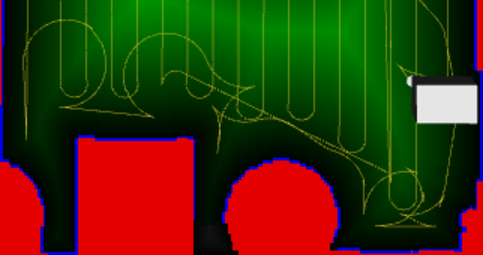
\includegraphics[width=1.00000\textwidth]{imgs/toolong.png}
\caption{Exemple de trajectoire de suivi des murs générée par
l'algorithme de Reeds and Sheep étonnamment longue}\label{fig:toolong}
\end{figure}

Notre objectif est alors de raccourcir au maximum la longueur de la
trajectoire finale, quitte à relaxer un peu la contrainte de couverture
de la surface.

Pour cela, nous remarquons que dans le cas classique d'un angle droit
entre deux murs, le robot balaye le premier mur jusqu'à la collision
avec le second, puis fait marche arrière, va se placer parallèlement au
second, refait marche arrière jusqu'à la collision avec le premier, puis
commence le balayage du second.

Cette manœuvre parait naturelle si l'on cherche à tout nettoyer au
mieux, mais demande beaucoup de temps. On nous demande alors de tronquer
la fin de la première trajectoire de balayage des bordures et le début
de la seconde.

Nous relions ensuite ces deux configurations par une trajectoire de
Dubins (Dubins \protect\hyperlink{ref-dubins}{1957}), qui est optimale
pour un robot mobile à tourelle ayant et rayon de giration borné et ne
se déplaçant qu'en marche avant\footnote{En pratique, vu que le robot
  balaye en marche arrière, nous parlons plutôt d'une trajectoire de
  Snibud.}.

Cette stratégie est illustrée sur la fig.~\ref{fig:dubins}

\begin{figure}
\centering

\hspace*{\fill}
\subfloat[Avant: Trajectoires complètes de balayage des murs, reliées
par une trajectoire de Reeds and
Sheep]{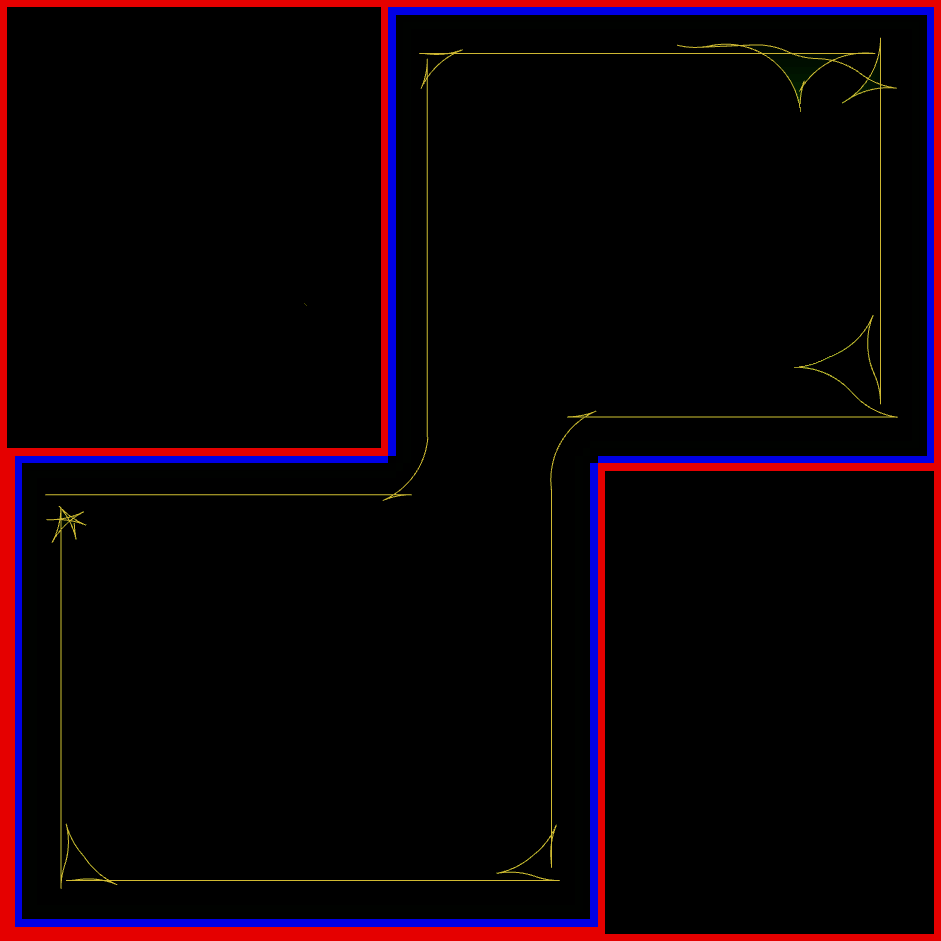
\includegraphics[height=5.00000cm]{imgs/avant.png}} \hfill%
\subfloat[Après: Trajectoires tronquées de balayage des murs dans
l'angle droit, reliées par une trajectoire de
Dubins]{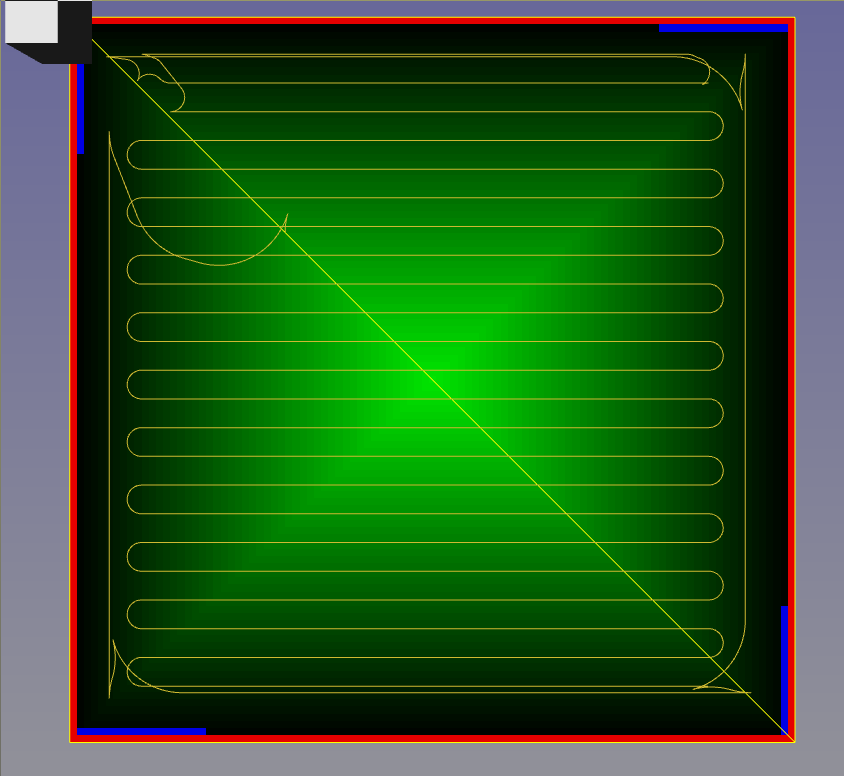
\includegraphics[height=5.00000cm]{imgs/apres.png}}
\hspace*{\fill}

\caption{Illustration du raccourci utilisé dans les angles droits.}

\label{fig:dubins}

\end{figure}

Dans le cas d'un angle droit, cette solution donne les bons résultats
auxquels nous nous attendions. Mais en pratique, il faut garder à
l'esprit que cela ajoute un paramètre supplémentaire à régler, à savoir
la longueur tronquée sur chaque trajectoire (voire deux si on veut des
longueurs tronquées différentes).

Or la valeur optimale de ce paramètre dépend grandement d'autres
paramètres, et notamment de l'angle entre deux murs successifs, de la
longueur initiale des trajectoires avant troncage, et de la distance
nécessaire entre le robot et le mur pour pouvoir tourner directement
sans engendrer de collision.

\section{Résultats}\label{sec:lemonres}

Dans le cadre de ce projet, nous avons développé des classes et méthodes
spécifiques au problème posé, nous les avons intégrées avec les classes
et méthodes déjà disponibles dans HPP, puis nous avons réglé
empiriquement les différents paramètres afin d'obtenir des trajectoires
le plus satisfaisantes possible sur les exemples fournis ainsi que sur
certains cas d'école.

Le résultat est un programme qui, dans la plupart des cas, produit une
trajectoire couvrant bien la surface à nettoyer, mais qui souvent
produit des trajectoires plus longues que nécessaire.

\subsection{Limitations}\label{limitations}

Comme nous l'avons vu dans la sec.~\ref{sec:bordures}, nous recherchons
pour l'instant uniquement des segments de droite, voire des arcs de
cercles dont le rayon doit être connu à priori.

Cependant, dans certains cas où plusieurs petits segments sont proches
les uns des autres, les transformées de Hough peuvent rater des segments
de droites pourtant évidents pour un humain.

Aussi, cette transformée de Hough implique un choix des paramètres de
discrétisation \((N_\rho, N_\theta)\). Pour pouvoir bien construire une
carte, il est donc souvent nécessaire de bien comprendre la théorie de
la transformée afin d'adapter ces paramètres à une zone donnée.

Sans cela, en utilisant des paramètres par défaut, des points alignés
peuvent se retrouver sur des droites différentes pour la transformée.
Cet effet peut être amplifié par le bruit inhérent à toute carte
construite à l'aide de capteurs.

En conséquence, cela implique des situations difficilement
compréhensibles pour un observateur extérieur où le robot balaye
plusieurs fois la même bordure.

Un autre problème vient de notre utilisation du RRT-Connect, qui peut
poser des problèmes dans le cas où la meilleure trajectoire suivante
peut éventuellement être à une grande distance. Cette situation s'est
notamment présentée dans l'un des exemples fournis, illustré dans la
fig.~\ref{fig:grandestation}.

\section{Travaux futurs}\label{sec:lemonfutur}

Lors de ce projet LEMON réalisé en coopération avec BA Systèmes, nous
avons tenté de répondre à un cahier des charges dans un temps limité par
le client final. Nous avons donc livré un logiciel fonctionnel, mais
sous-optimal.

Dans cette section, nous discutons des possibilités d'extension de ce
travail afin de rendre les trajectoires générées plus proches de celles
qui seraient réalisées par un être humain, voire meilleures.

\subsection{Suivi des murs}\label{suivi-des-murs}

Dans un premier temps, nous avons choisi de détecter des primitives
géométriques afin de suivre les bordures.

Une autre approche possible consisterait à extraire une trajectoire
directement de la forme des contours formés par les \texttt{Pixels} de
type \texttt{BOUNDARY}, en les reliant avec une trajectoire de Dubins.
Certains \texttt{Pixels} ne seraient pas atteignables, mais comme nous
l'avons vu dans la sec.~\ref{sec:optimisation}, ce n'est finalement pas
un problème.

Pour cela, l'idéal serait de pouvoir profiter du débattement de la
brosse latérale pour mieux gérer la distance entre le robot et le mur,
alors que jusqu'ici nous n'avons considéré qu'elle n'avait que deux
états possibles~: sortie pour le balayage des bordures et rentrée pour
le nettoyage des surfaces.

\subsection{Direction du nettoyage des surface et découpage de la zone
principale}\label{direction-du-nettoyage-des-surface-et-duxe9coupage-de-la-zone-principale}

Dans cette première version, nous avons choisi de nettoyer toutes les
surfaces selon la même direction, et en utilisant la direction donnée
par le plus grand coefficient de la première transformée de Hough. Dans
certains cas, cette direction n'est pas la meilleure, comme le montre le
contre-exemple sur la fig.~\ref{fig:diagonale}.

Par ailleurs, il peut être bon de découper la zone principale en
sous-zones présentant des directions générales différentes. Un
algorithme de découpage d'une zone non-convexe a déjà été développé dans
le cadre du travail d'engins agricoles dans (Tran, Taïx, et Souères
\protect\hyperlink{ref-decoupage}{2005}), dont est extrait la
fig.~\ref{fig:decoupage}.

\begin{figure}
\centering
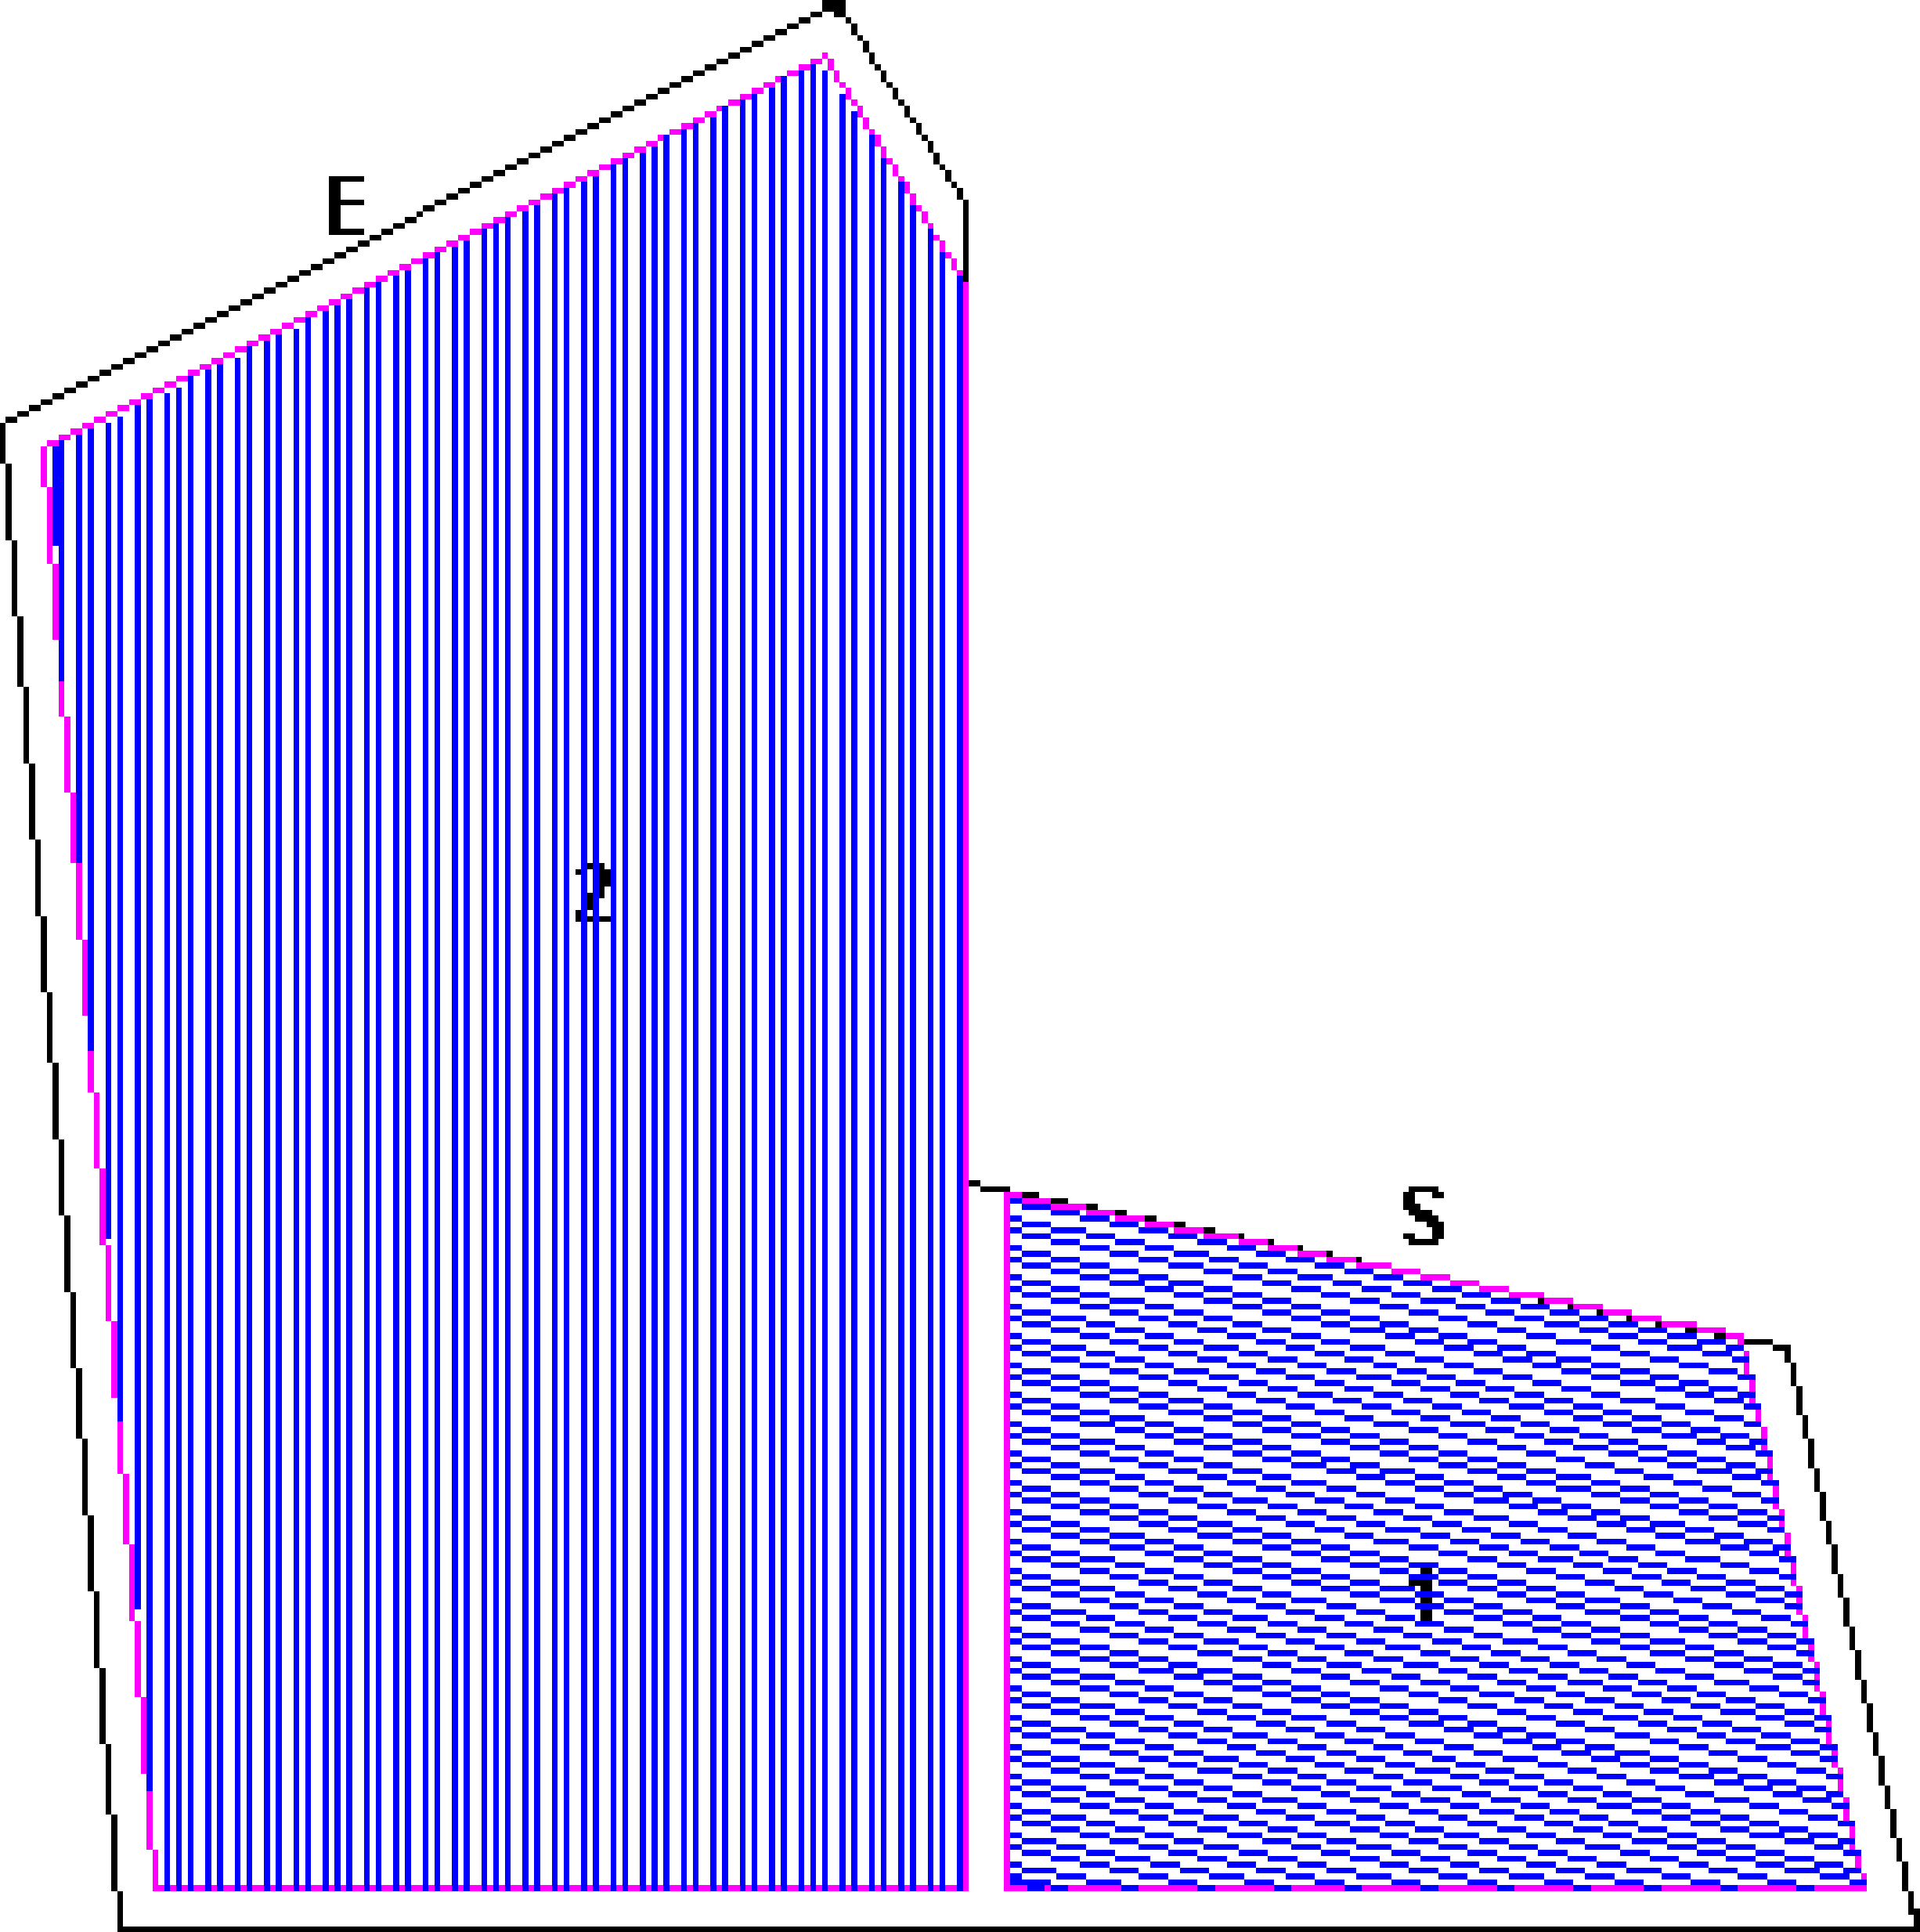
\includegraphics[width=1.00000\textwidth]{imgs/decoupage.png}
\caption{Exemple d'algorithme de planification de trajectoires pour
engin agricole dans des polygones non convexes}\label{fig:decoupage}
\end{figure}

\subsection{Ordre de parcours des portions de
trajectoires}\label{ordre-de-parcours-des-portions-de-trajectoires}

Un dernier axe d'amélioration serait d'optimiser l'ordre de parcours des
portions de trajectoires de balayage des bordures et de nettoyage des
surfaces.

Dans un premier temps, une modification d'algorithmes classiques de
recherche opérationnelle pourrait permettre de mieux prendre en compte
la possibilité de parcourir les trajectoires de nettoyage des surfaces
dans un sens ou dans l'autre, ainsi que de palier au problème de la
recherche de la trajectoire suivante si sa configuration initiale est
trop loin pour notre RRT-Connect.

Dans un second temps, l'idéal serait de pouvoir découper certaines
trajectoires de balayage des bordures pour aller balayer un obstacle
proche d'un long mur, comme dans la fig.~\ref{fig:pilierrond}.

\chapter{Robots mobiles tri-tourelles}\label{sec:transhumus}

Dans ce dernier chapitre sur la robotique mobile, nous faisons le
rapport d'un projet réalisé pour l'Institut Français, en coopération
avec les entreprises BA Systèmes et Ubisense. Il a consisté à
implémenter le contrôle et la planification de robots mobiles
omnidirectionnels.

Comme pour le projet \emph{off road} présenté dans le chapitre
\ref{sec:offroad}, les robots constituent une œuvre d'art de l'artiste
Céleste Boursier-Mougenot. Cette fois-ci, nous dotons de moyens de
locomotion trois pins sylvestres, de plusieurs mètres de haut et
plusieurs tonnes.

\section{Introduction}\label{sec:transintro}

La Biennale de Venise (Di Martino
\protect\hyperlink{ref-DiMartino}{2005}) est la plus importante
exposition d'art contemporain au monde. Elle a lieu une fois tous les
deux ans depuis 1895. L'exposition est répartie dans différents lieux à
Venise, parmi lesquels les \emph{Giardini} comportant 90 pavillons,
étant chacun dirigés par une nation.

Pour la 56\textsuperscript{ième} édition en 2015, l'Institut Français,
en charge du pavillon français, a choisi le projet Rêvolutions de
l'artiste Céleste Boursier-Mougenot et la commissaire Emma Lavigne. Ce
projet incluait l'œuvre transHumUs dont nous parlons dans ce chapitre.

Dans transHumUs, l'artiste a voulu créer une chorégraphie de trois
arbres mobiles se déplaçant en fonction de leur métabolisme, et a choisi
la variation du flux de leur sève lorsqu'ils passent de l'ombre à la
lumière. Ce spectacle a eu lieu de mai à novembre, six jours par
semaine, huit heures par jour.

La fig.~\ref{fig:transhumusintro} présente respectivement l'idée
initiale et la réalisation finale du projet. Neuf mois séparent les deux
images. L'objectif de ce chapitre est de faire le rapport sur la
recherche et le développement qui ont été conduits pendant cette
période, depuis notre première réunion avec l'artiste jusqu'au
vernissage de l'exposition le 5 mai 2015.

\begin{figure}
\centering

\hspace*{\fill}
\subfloat[Vue
d'artiste]{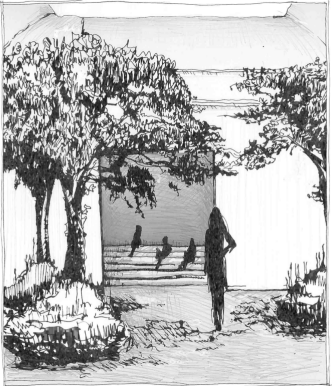
\includegraphics[height=4.50000cm]{imgs/dessin.png}} \hfill%
\subfloat[Résultat
final]{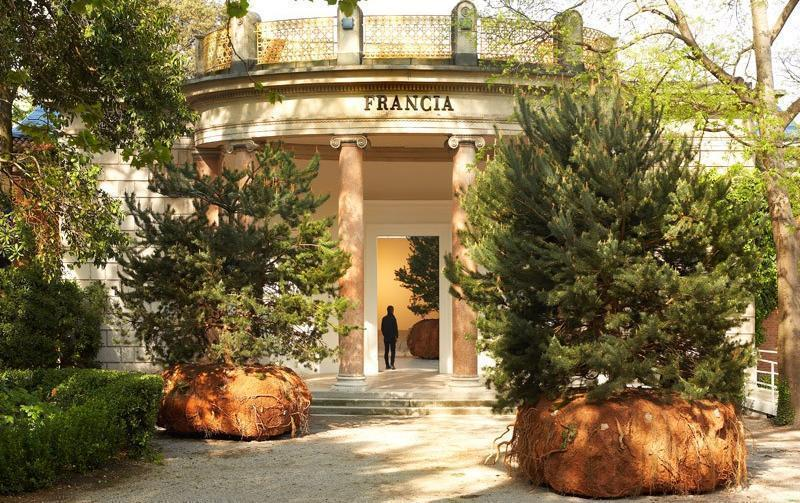
\includegraphics[height=4.50000cm]{imgs/couverture.jpg}}
\hspace*{\fill}

\caption{Des spécifications à la réalisation. Neuf mois séparent les
deux images.}

\label{fig:transhumusintro}

\end{figure}

Comment transcrire la dimension poétique de ce projet en des termes
technologiques ? La question s'adresse à tous les composants d'un
système robotique, de la conception de machines capables de déplacer
trois tonnes (l'arbre, ses racines, et la terre nécessaire),
l'architecture de perception qui doit combiner des capteurs
égocentriques et allocentriques, et le système de génération de
mouvement qui doit retranscrire le critère de qualité du mouvement
défini par l'artiste en termes de lissage de trajectoire et de vitesse.

Notre contribution dans ce projet a été de sélectionner les fournisseurs
(sec.~\ref{sec:transspecs}), développer un architecture logicielle
comprenant une interface-utilisateur pour l'équipe du pavillon
(sec.~\ref{sec:transarchi}) et s'occuper de la gestion du projet
(sec.~\ref{sec:transresults}).

Notre seconde contribution a été de proposer à l'artiste des stratégies
de génération et de planification du mouvement donnant l'impression que
les arbres errent en totale autonomie (sec.~\ref{sec:transplanif}).

\section{Spécifications et solutions techniques}\label{sec:transspecs}

L'ambition poétique de ce projet est de libérer les arbres de leur
immobilité et de les laisser explorer le monde par eux-mêmes. Cette
ambition impose la création de connections originales entre des éléments
naturels et technologiques.

Cette inspiration continue le travail de Céleste Boursier-Mougenot de
ces dernières années (MacAdam \protect\hyperlink{ref-MacAdam}{2015}).

La première étape de ce projet a été d'ouvrir un processus de dialogue
avec l'artiste. Nous avons ainsi dû définir le type d'arbres utilisés,
leur occupation de l'espace dans les \emph{Giardini}, ce que signifie
pour un arbre de bouger «~de lui-même~», et quelles sont les conditions
de développement et d'exploitation.

\subsection{Spécifications}\label{spuxe9cifications}

Les spécifications qui suivent dans cette section sont issues de ce
processus de dialogue avec l'artiste.

\subsubsection{Arbres}\label{arbres}

Les arbres retenus pour ce projet sont des pins sylvestres, dont la
floraison en mai coïncide avec l'ouverture de la Biennale. Nous avons
donc pris trois de ces arbres pour l'œuvre à Venise, plus un pour nos
tests au LAAS-CNRS.

Ils font environ cinq mètres de haut. Ils sont vivants, et se déplacent
avec leur motte de terre pour un total d'environ trois tonnes.

\subsubsection{Zones}\label{zones}

Deux de ces arbres évoluent dans l'espace devant les pavillons français,
anglais, canadien et allemand. Ils doivent rester à l'intérieur d'une
zone de 300 mètres carrés bien définie (fig.~\ref{fig:zones}). Le sol de
cette zone est composée de terre battue et de graviers, donc sa dureté
dépend des conditions météorologiques.

\begin{figure}
\centering

\hspace*{\fill}
\subfloat[Vue aérienne des pavillons français (sur la gauche), anglais
(en haut au centre), canadien (en haut à droite) et allemand (sur la
droite) autour d'une esplanade dans les
\emph{Giardini}]{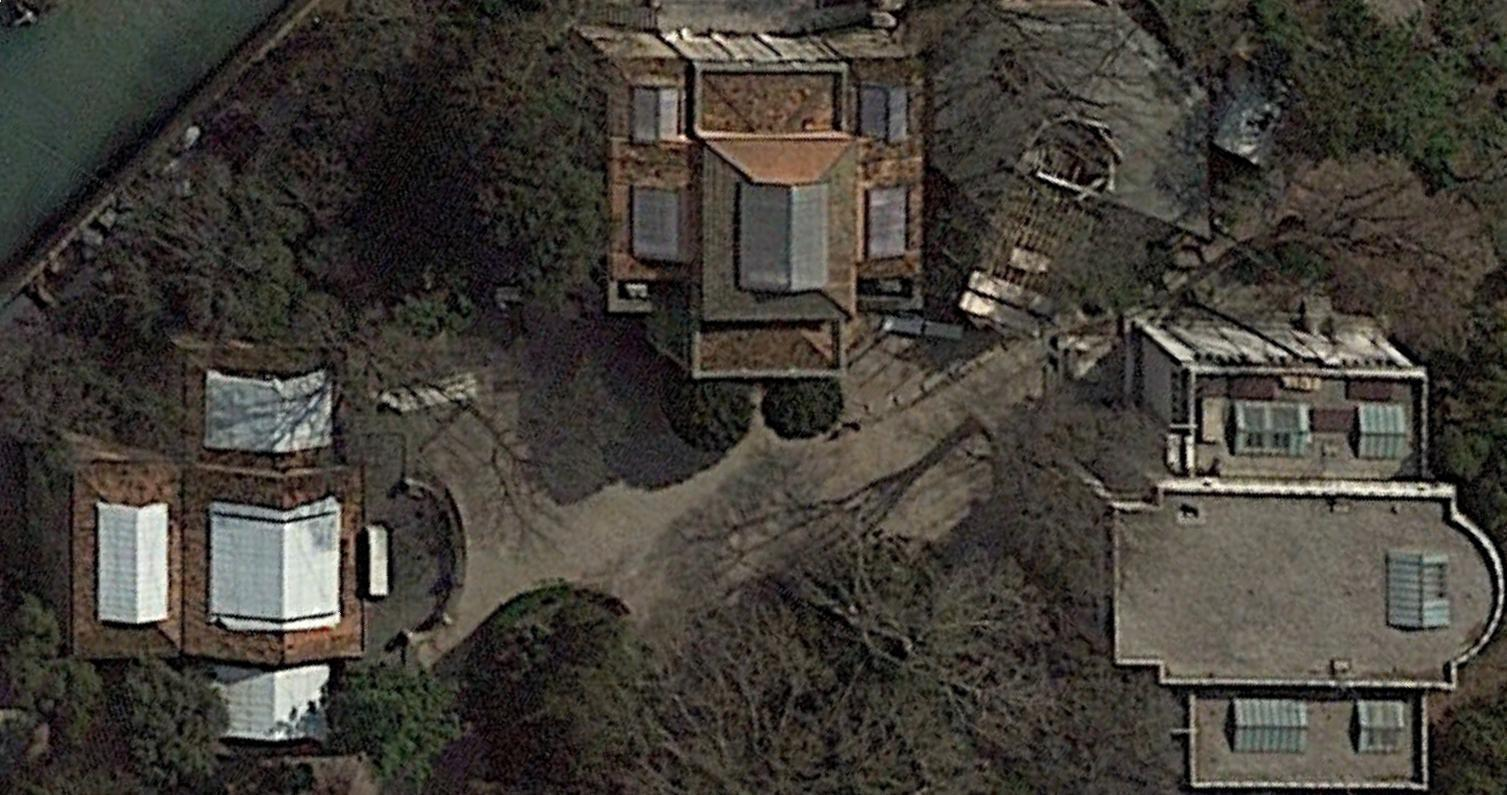
\includegraphics[width=1.00000\textwidth]{imgs/earth.jpg}}
\hspace*{\fill}

\hspace*{\fill}
\subfloat[Modèle géométrique des zones d'évolution, avec une grille dont
les carreaux font 10 mètres pour l'échelle. Cette image est issue de
l'interface-utilisateur servant à monitorer le déplacement des
arbres.]{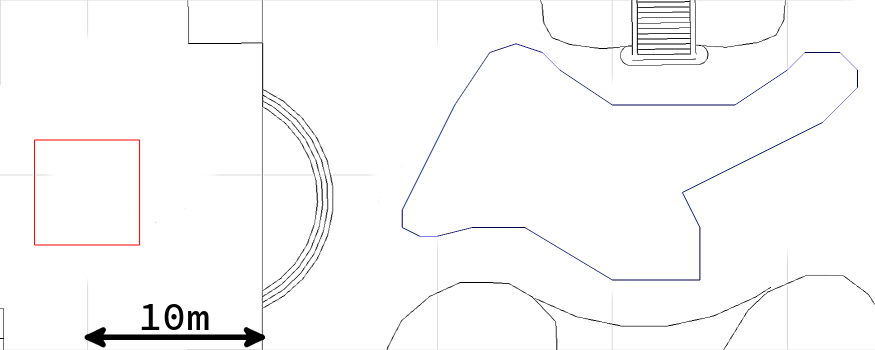
\includegraphics[width=1.00000\textwidth]{imgs/plan_vierge.png}}
\hspace*{\fill}

\caption{Vue aérienne de la partie des \emph{Giardini} qui nous
intéresse. Le pavillon français est le bâtiment sur la gauche. Un arbre
se déplace dans la salle principale de ce pavillon, et les deux autres
se partagent l'esplanade commune aux pavillons anglais, canadien et
allemand.}

\label{fig:zones}

\end{figure}

Le troisième arbre se déplace lui dans le pavillon français, dans une
zone de 50 mètres carrés pourvue d'un sol en béton.

Ces deux zones ne comportent pas d'obstacles permanents, mais sont des
aires de passage de visiteurs sans contraintes spécifiques de sécurité.
Ces visiteurs sont autorisés à approcher et toucher les arbres.

\subsubsection{Origine du mouvement}\label{origine-du-mouvement}

Les arbres sont des êtres vivants, dont le métabolisme dépend des
conditions environnementales et météorologiques. Leur mouvement doit
dépendre des variations de leur état interne. Ceci est l'une des
principales problématiques de ce projet: cette œuvre cherche à révéler
l'invisible état interne des arbres.

Il est également nécessaire de restreindre le mouvement des arbres aux
zones définies dans la section précédente, et d'éviter les collisions
entre les deux arbres qui partagent l'esplanade.

\subsubsection{Qualité du mouvement}\label{qualituxe9-du-mouvement-1}

L'artiste tient à ce que les arbres bougent extrêmement lentement. Avec
une vitesse inférieure au mètre par minute, leurs mouvements doivent
être à peine perceptibles. Les arbres doivent bouger sans avoir une
direction privilégiée: ils devraient être holonomes.

Aucun bruit ne doit être audible pour les visiteurs, les arbres doivent
donner l'impression de se mouvoir par lévitation. La base de la motte de
terre doit être à moins de 5cm du sol.

\subsubsection{Contraintes
opérationnelles}\label{contraintes-opuxe9rationnelles}

Le projet doit être réalisé en six mois sans aucune extension possible
de date limite, fixée à l'ouverture de la biennale, le 5 mai 2015, avec
seulement deux semaines de tests sur site.

L'œuvre doit fonctionner jusqu'au 22 novembre 2015, à raison de 8 heures
par jour et 6 jours par semaine. Elle doit être utilisable par l'équipe
de non-spécialistes du pavillon français en une journée de formation.

\subsection{Solutions technologiques}\label{solutions-technologiques}

Ces spécifications ont conduit aux solutions technologiques suivantes.

\subsubsection{Conception de la
plate-forme}\label{conception-de-la-plate-forme}

Des plate-formes robotiques sur mesure ont été conçues par BA Système,
une société spécialisée dans la conception et la production d'AGV
(Automatic Guided Vehicles) pour la logistique.

Chaque plate-forme est composée d'un bac octogonal supporté par trois
tourelles, composées d'une roue motrice électrique, orientable autour de
son axe central. Les roues peuvent donc tourner sur place.

Le bruit des moteurs électriques de traction et d'orientation sont
inaudibles.

Cela ne rend pas la plate-forme holonome, mais bien omnidirectionnelle,
de type \((1, 2)\) dans la classification de (Campion, Bastin, et
Dandrea-Novel \protect\hyperlink{ref-campion96}{1996}). On peut donc
contrôler la plate-forme dans chacune des trois directions de
\(\mathbb{R}^2\times S^1\). Le modèle de contrôle utilisé est présenté
dans la sec.~\ref{sec:transmodel}.

Les mottes des arbres sont insérées dans les bacs, et des coquilles
synthétiques imitant la terre et les racines encapsulent les AGVs. Les
coques synthétiques contribuent également à la suppression totale de
légers bruits qui pourraient provenir des moteurs.

\begin{figure}
\centering
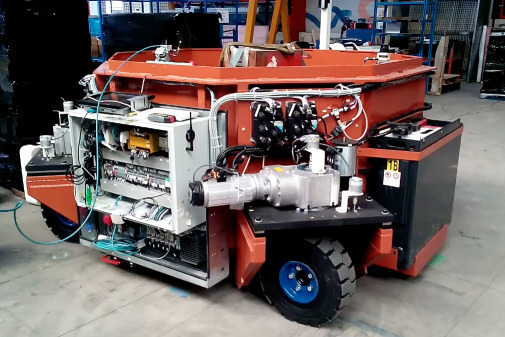
\includegraphics[width=1.00000\textwidth]{imgs/capture_video_BA.jpg}
\caption{AGV dans les locaux de BA Systèmes}
\end{figure}

\subsubsection{Capteur du métabolisme des
arbres}\label{capteur-du-muxe9tabolisme-des-arbres}

La sonde Granier (Granier \protect\hyperlink{ref-granier}{1987})
(fig.~\ref{fig:needles}) est l'une des techniques les plus courantes
pour mesurer le métabolisme d'un arbre (P. Lu
\protect\hyperlink{ref-lu2004}{2004}). La sonde est fondée sur un
principe de dissipation thermique, et est constituée de deux aiguilles.

Une aiguille chauffée est placée dans l'aubier au-dessus d'une aiguille
neutre. Quand la vitesse de la sève est faible, la chaleur de l'aiguille
chauffée est peu dissipée, et la différence de température entre les
deux aiguilles est donc élevée. Cette différence diminue avec
l'augmentation de la vitesse de la sève.

Sur le pin sylvestre installé au LAAS-CNRS, nous avons vérifié que la
sensibilité de ces sondes était suffisante pour observer une différence
de luminosité.

Cette luminosité change avec les conditions atmosphériques, ainsi que
lorsque que l'arbre se déplace entre l'ombre et la lumière. Nous
installons alors dans chaque arbre trois sondes dans différentes
directions. Les mesures données par les sondes sont ensuite utilisées
comme des entrées pour la génération de mouvement
(fig.~\ref{fig:mesures}).

\begin{figure}
\centering

\hspace*{\fill}
\subfloat[Capteurs de flux de sève: les sondes Granier sont composées de
deux aiguilles
thermocouples]{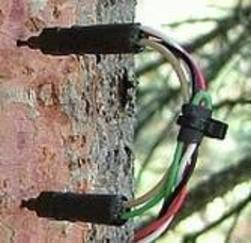
\includegraphics[width=5.00000cm]{imgs/sapflow.jpg}\label{fig:needles}}
\hfill%
\subfloat[Déplacement d'un arbre de l'ombre à la lumière et vice-versa:
mesures d'une sonde Granier sur l'arbre de test au LAAS-CNRS les 8 et 9
avril 2015, entre 12:00 et 18:00, lorsque l'on déplace l'arbre aux
alentours de
15:00.]{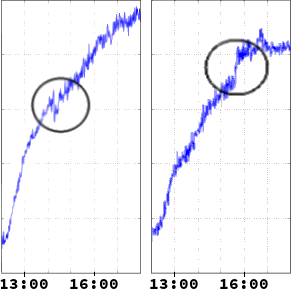
\includegraphics[height=4.00000cm]{imgs/granier.png}\label{fig:mesures}}
\hspace*{\fill}

\caption{Mesures du flux de sève: ces expériences nous ont permis de
vérifier cette solution technique par rapport à nos spécifications. Nous
avons constaté que la réaction d'un arbre passant de l'ombre à la
lumière était mesurable et donc exploitable en tant qu'entrée de notre
système, puisque le métabolisme des arbres peut influer sur leur
déplacement.}

\label{fig:granier}

\end{figure}

\subsubsection{Localisation}\label{sec:transloc}

Les aires d'évolution sont définies à l'intérieur et à l'extérieur du
pavillon français. Pour localiser les AGV, nous avons donc opté pour une
technologie UWB (Ultra Wide Band) développée par la société Ubisense.
Cette technologie nous apporte un bon compromis entre la précision et la
discrétion.

Les bâtiments autour des zones d'évolution des arbres sont équipés
d'antennes assurant une couverture complète (fig.~\ref{fig:ubisense}).
Les arbres sont équipés de plusieurs petits récepteurs cachés dans les
branches. Une précision de l'ordre de 15 centimètres est obtenue avec un
bon niveau de qualité.

\begin{figure}
\centering
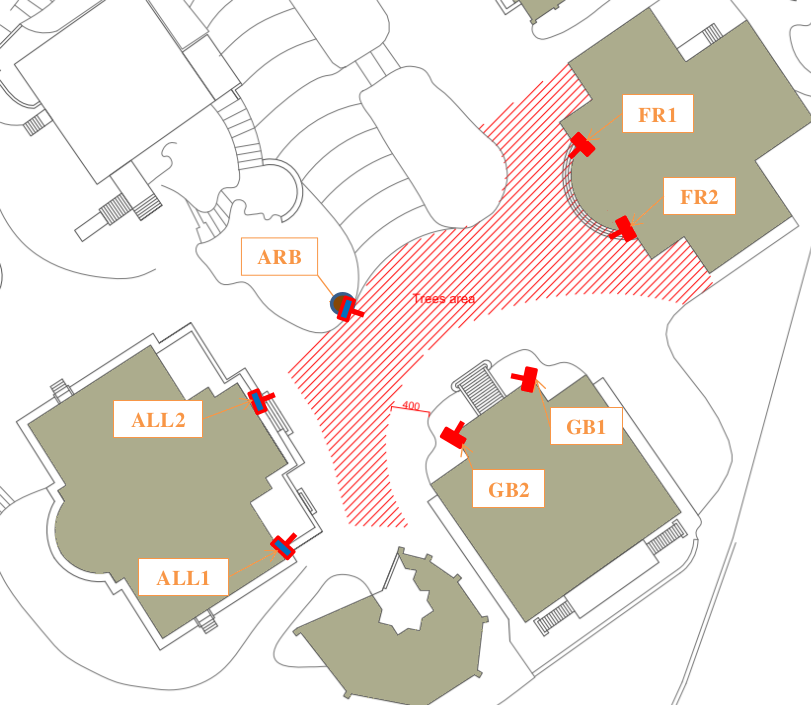
\includegraphics[height=7.00000cm]{imgs/plan_capteurs.png}
\caption{Implantation des antennes UWB Ubisense dans les
\emph{Giardini}}\label{fig:ubisense}
\end{figure}

\section{Architecture logicielle}\label{sec:transarchi}

Dans la section précédente, nous avons détaillé notre choix de
fournisseurs de solutions matérielles. Nous étions également en charge
de la gestion des principaux développements logiciels. La
fig.~\ref{fig:soft} récapitule les différents composants du système et
les flux de données entre eux.

\begin{figure}
\centering
\includegraphics[width=1.00000\textwidth]{tikz/schema_block.pdf}
\caption{Architecture logicielle: chaque arbre a trois sondes Granier
qui sont utilisées par le planificateur de trajectoire. Le planificateur
de trajectoire récupère également la position et l'orientation actuelle
de chaque robot grâce au système de géolocalisation, puis calcule les
vitesses de traction et d'orientation de chaque tourelle de chaque AGV.
Un utilisateur peut aussi directement donner des consignes au
planificateur de trajectoire lorsque c'est nécessaire. Les variables
\((s_1, s_2, s_3)\), \((x, y, \alpha)\) et \((v_i, \theta_i)\) sont
explicitées dans la sec.~\ref{sec:transplanif}}\label{fig:soft}
\end{figure}

Les logiciels ont été développés pour être le plus modulaire possible.
Il est donc facile de passer des cas de tests en simulation aux cas de
production. Cette modularité permet également de surmonter la diversité
de technologies utilisées par nos fournisseurs, puisque des
convertisseurs sont simples et rapide à coder.

En effet, les sondes Granier fournissent des valeurs toutes les 30
secondes sur une liaison série, le logiciel des AGV attend des commandes
ASCII sur un socket TCP, et la suite logicielle de géolocalisation est
bâtie sur une technologie .NET qui ne peut être étendue que via des
modules d'un cadre logiciel propriétaire dont la fréquence
d'actualisation peut aller de 1 à 100 hertz.

Par conséquent, nous avons utilisé une architecture logicielle fondée
sur la librairie de messagerie ZeroMQ (Hintjens
\protect\hyperlink{ref-zeromq}{2013}), qui peut être utile pour tous nos
canaux de communication. Cette librairie est disponible dans plusieurs
langages de programmation, et fournit une abstraction aux problématiques
de connections / déconnections des sockets sous-jacentes. Enfin, elle
implémente des schémas de communication classiques tels que
\emph{Client/Server}, \emph{Publish/Subscribe} et \emph{Push/Pull}.

L'idée générale de notre architecture est d'avoir un planificateur de
trajectoire qui est un composant central, et qui est capable d'effectuer
des \emph{Pull} depuis les entrées et des \emph{Publish} vers les
sorties. Ainsi les autres composants peuvent se mettre à récupérer des
données via des \emph{Subscribe} et en envoyer grâce à des \emph{Push} à
tout moment, sans perturber le processus principal. Certaines
fonctionnalités périphériques peuvent également être ajoutées à la volée
en étant à la fois un \emph{Subscriber} et un \emph{Pusher}.

Une interface-utilisateur graphique fondée sur des technologies web a
également été développée pour aider l'équipe du pavillon à voir la
situation actuelle, et gérer les éventuels problèmes qui pourraient
arriver (fig.~\ref{fig:simulateur-right}).

\begin{figure}
\centering
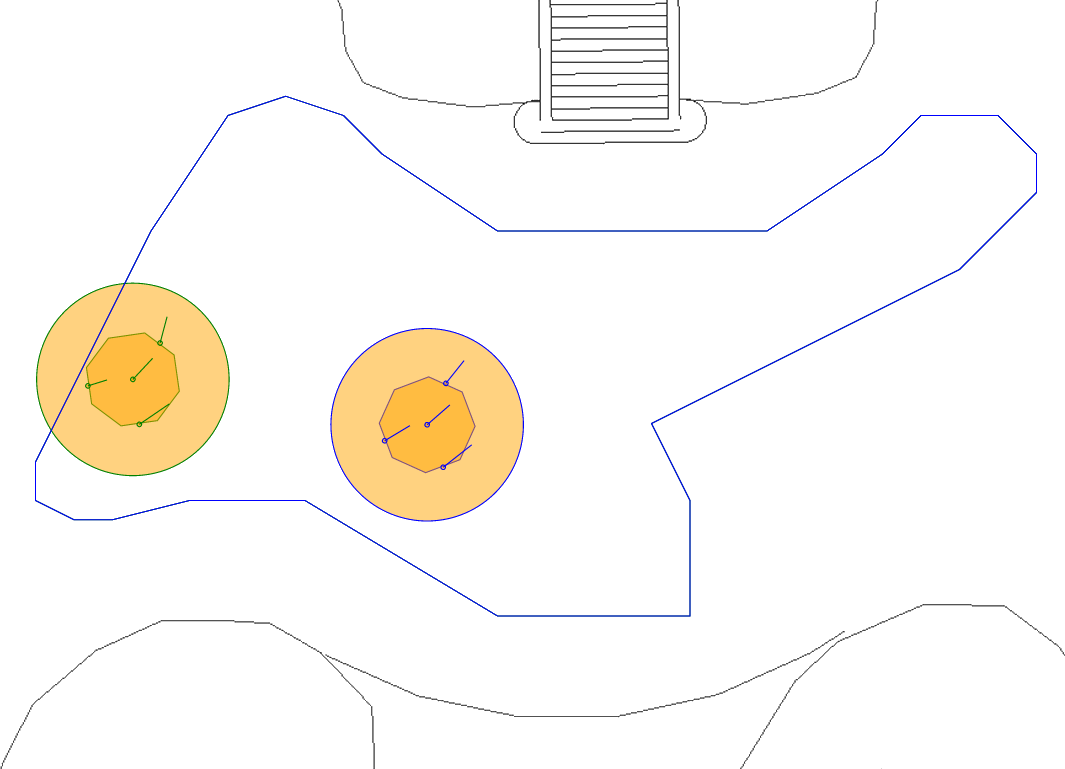
\includegraphics[width=1.00000\textwidth]{imgs/simulateur-right.png}
\caption{Exemple d'utilisation de l'interface utilisateur web, affichant
la situation actuelle: deux AGVs se déplacent sur l'esplanade, et on
peut voir leur position et orientation, ainsi que l'orientation et la
vitesse de traction des tourelles.}\label{fig:simulateur-right}
\end{figure}

Dans des cas plus complexes, ceci nous permet également de travailler
sur l'installation à distance, pour éviter d'avoir besoin d'ingénieurs
sur place. Enfin, pendant la période de développement, cette interface a
également permis à l'artiste de se faire une idée du mouvement des
arbres au fur et à mesure de notre avancement.

\emph{NB:} En temps normal, cette interface-utilisateur est inutile, vu
que le système est entièrement autonome.

\section{Planification de mouvement et contrôle}\label{sec:transplanif}

Dans cette section, nous explicitons la manière dont est générée le
mouvement des plate-formes robotiques supportant les arbres.

Pour cela, nous commençons par la modélisation mathématique de la
gestion des orientation et vitesses de traction des tourelles, dans la
sec.~\ref{sec:transmodel}, puis nous voyons comment nous générons le
mouvement à partir des sondes Granier dans la sec.~\ref{sec:transgene}
et nous ajoutons certaines fonctions de lissage dans la
sec.~\ref{sec:translissage}. Pour finir, nous expliquons comment nous
faisons en sorte que l'arbre «~choisisse~» sa destination, dans la
sec.~\ref{sec:transgoal}.

\subsection{Modélisation de la plate-forme}\label{sec:transmodel}

Comme nous l'avons vu dans la sec.~\ref{sec:transspecs} , l'artiste
désire un mouvement omnidirectionnel. Nous avons donc besoin de trois
variables d'entrée, ce qui correspond à la classe de robot mobile
\((1, 2)\).

Puisque l'artiste désire que le robot n'ait pas une direction
privilégiée du mouvement, nous choisissons un système de coordonnées
polaires en \((v, \theta, \omega)\), où:

\begin{itemize}
\tightlist
\item
  \(\theta \in [-\pi, \pi[\) est la direction dans laquelle se déplace
  le centre de l'AGV;
\item
  \(v \in [0, 1]\) est sa vitesse linéaire dans la direction \(\theta\);
\item
  \(\omega \in [-1, 1]\) est sa vitesse angulaire.
\end{itemize}

Avec ce système de coordonnées, on peut facilement calculer la sortie
demandée par l'AGV, qui est la direction \(\theta_i\) et la vitesse de
traction \(v_i\) de chaque roue \(i\), comme le montre
l'eq.~\ref{eq:agv}:

\begin{equation} \begin{aligned}
    v_{x_i} &= v \cos(\theta)- \omega R_i \sin(\alpha_i) \\
    v_{y_i} &= v \sin(\theta)+ \omega R_i \cos(\alpha_i) \\
    v_i &= \sqrt{v_{x_i}^2 + v_{y_i}^2} \\
    \theta_i &= \operatorname{atan2}(v_{y_i}, v_{x_i})
\end{aligned} \label{eq:agv}\end{equation}

Dans l'eq.~\ref{eq:agv}, \((R_i, \alpha_i)\) est la position angulaire
de la roue \(i\), comme on peut le voir sur la fig.~\ref{fig:octogons}

\begin{figure}
\centering

\hspace*{\fill}
\subfloat[De \((v, \theta, \omega)\) à
\((v_i, \theta_i)\)]{\includegraphics{tikz/octogon_1.pdf}\label{fig:octogon1}}
\hfill%
\subfloat[Construction
géométrique]{\includegraphics{tikz/octogon_2.pdf}\label{fig:octogon2}}
\hspace*{\fill}

\caption{\((v_i, \theta_i)\) en fonction de \((v, \theta, \omega)\) et
\((R_i, \alpha_i)\)}

\label{fig:octogons}

\end{figure}

Avec cette construction, on peut assurer l'unicité du centre instantané
de rotation, et que donc on ne risque pas de se retrouver dans une
situation ou les tourelles risquent d'écarteler un AGV, comme on peut le
voir sur la fig.~\ref{fig:octogon3}

\begin{figure}
\centering
\includegraphics{tikz/octogon_3.pdf}
\caption{Centre Instantané de Rotation (CIR)}\label{fig:octogon3}
\end{figure}

\subsection{Génération de mouvement}\label{sec:transgene}

D'après les spécifications établies avec l'artiste, la génération du
mouvement doit provenir du métabolisme de l'arbre. Et comme nous venons
de le voir, nous avons besoin de trois variables indépendantes d'entrée.
Nous choisissons donc d'utiliser les signaux de trois sondes Granier
implantées à différents endroits de l'arbre, que nous notons
\((s_1, s_2, s_3)\) et normalisons dans \([0, 1]\).

Deux de ces sondes peuvent être directement connectées aux vitesses
linéaire et angulaire du centre de l'AGV, comme on peut le voir dans
l'eq.~\ref{eq:speeds}:

\begin{equation} \begin{aligned}
    v &= s_1 \\
    \omega &= 2s_2 - 1
\end{aligned} \label{eq:speeds}\end{equation}

Les unités de ces vitesses sont ensuite déduites pour satisfaire les
spécifications sur la vitesse générale de l'arbre. Dans ce cas, la
vitesse maximale du tronc de l'arbre est d'un mètre par minute (soit
environ 17 millimètres par seconde), mais les roues de l'AGV peuvent
aller jusqu'à deux mètres par minute. Par conséquent, nous n'avons qu'à
multiplier chaque \(v_i\) par 17mm/s avant de les envoyer à l'AGV.

Une stratégie globale de génération de mouvement a été établie avec
l'artiste, et implique que l'arbre se «~souvienne~» à quel endroit l'une
des variables de son métabolisme était à son maximum ou son minimum. Un
arbre ira donc alternativement chercher le soleil et l'ombre, en
fonction de ses sondes Granier, dans un lieu où il se souvient de l'état
de son flux de sève, ou dans un lieu où il n'est pas encore allé.

La principale composante de la génération de trajectoire est donc le
paramètre \(\theta\). La géolocalisation donne la position et
l'orientation absolue \((x, y, \alpha)\) de l'AGV, donc une fois que la
destination \((x_{goal}, y_{goal})\) est déterminée grâce à la dernière
sonde Granier, on peut obtenir ce paramètre \(\theta\) suivant
l'eq.~\ref{eq:theta}.

\begin{equation}
\theta = \left(\operatorname{atan2}\left(y - y_{goal}(s_3), x - x_{goal}(s_3)\right) - \alpha\right) \% 2 \pi - \pi
\label{eq:theta}\end{equation}

Ce principe règle le problème de couverture de l'espace et est développé
dans la sec.~\ref{sec:transgoal}.

\subsection{Lissage}\label{sec:translissage}

Au-dessus de ce principe basique de génération de mouvement, nous
implémentons un composant de lissage qui contrôle la vitesse angulaire
maximale de chaque roue. En effet, les deux AGVs qui évoluent sur
l'esplanade peuvent facilement s'embourber, et notamment en tournant
leurs roues trop brutalement, creusant ainsi le sol sous leurs roues.

De son côté, l'AGV à l'intérieur du pavillon français peut produire un
bruit strident fort désagréable lorsque son pneu crisse sur le béton,
toujours s'il tourne trop vite.

Si ce composant détecte que la différence entre la direction d'un AGV et
la direction du \(goal\) est supérieure à \(2\pi/3\), il peut également
inverser le sens de rotation des roues pour n'avoir à tourner que de
moins de \(\pi/3\). Ceci améliore notamment le comportement aux points
de rebroussement, lorsque l'AGV change de \(goal\).

Un composant similaire est implémenté sur l'AGV au niveau de chaque
tourelle, tout en assurant que le centre instantané de rotation reste
unique.

\subsection{Sélection du but}\label{sec:transgoal}

La génération de mouvement définit comment un AGV évoluerait seul sur un
plan infini. Nous avons ajouté certaines règles pour nous assurer que la
sélection du \(goal\) ne fera pas aller un AGV dans un mur ou un autre
AGV. Ces règles sont détaillées dans l'alg. \ref{alg:goal}, mais l'idée
générale est de mettre à jour en continu deux cartes de l'aire
d'évolution avec le \(timestamp\) et \(s_3\) dans la case correspondant
aux coordonnées actuelles.

\begin{algorithm}
\caption{Génération de mouvement et de trajectoire}
\label{alg:goal}
\begin{algorithmic}[1]

\Loop
    \State \emph{start\_loop}:
    \Comment{Label du début}
    \State $map_{sap flow}[position] \gets s_3$
    \Comment{Mise à jour de cartes}
    \State $map_{timestamp}[position] \gets timestamp$
    \If {$\Vert goal - position\Vert < 1$}
        \Comment{Besoin d’un nouveau $goal$}
        \For {$try \gets 1, N$}
            \If {$state = 1$}
                \State $goal \gets \arg\min(map_{sap flow})$
            \ElsIf {state = 2}
                \State $goal \gets \arg\max(map_{sap flow})$
            \Else
                \State $goal \gets \arg\min(map_{timestamp})$
            \EndIf
            \State $state \gets (state + 1) \% 3$
            \If {\Call{clearpath}{$goal - position$}}
                \State \textbf{goto} \emph{continue}
                \Comment{Le nouveau $goal$ convient}
            \EndIf
        \EndFor
        \State $goal \gets position$
        \Comment{Échec de recherche d’un nouveau $goal$}
        \State $v \gets 0$
        \State $\omega \gets s_2$
        \Comment{L’arbre peut continuer de tourner sur place}
        \State sleep 10s
        \State \textbf{goto} \emph{start\_loop}
        \Comment{Nouvelle tentative}
    \EndIf
    \State \emph{continue}:
    \Comment{Label de succès}
    \State $v \gets s_1$
    \State $\omega \gets s_2$
    \Comment{Voir \ref{sec:transgene}}
    \State $\theta_{goal} \gets \left(\operatorname{atan2}\left(y - y_{goal}(s_3), x - x_{goal}(s_3)\right) -
    \alpha\right) \% 2 \pi - \pi$
    \State sleep 1s
\EndLoop
\Procedure{clearpath}{$trajectory$}
    \Comment{Pas d’obstacle entre $position$ et $goal$}
    \State \Return $trajectory \cap (borders \cup {trajectory}_{other AGV}) = \varnothing$
\EndProcedure

\end{algorithmic}
\end{algorithm}

De cette manière, nous obtenons des cartes \(map_{sapflow}\) et
\(map_{timestamp}\) indiquant les zones où la sève a coulée rapidement
ou non (qui coïncideront probablement avec les zones d'ombre et de
soleil), et les zones où un AGV n'est pas allé depuis longtemps.

Ensuite, une machine d'états finis alterne le \(goal\) entre des
endroits où \(s_3\) était maximum, puis minimum, puis un endroit où
l'arbre n'est pas allé depuis longtemps.

Dans certaines circonstances, il est possible qu'aucune de ces zones ne
soit atteignable en ligne droite, sans traverser de bordure, ou de
trajectoire d'un autre AGV. Dans un tel cas de \emph{deadlock}, l'AGV
doit simplement attendre dans sa position courante.

Les traces générées par cet algorithme en simulation sont données dans
la fig.~\ref{fig:ressimulation}.

Un des objectifs de la génération de trajectoire est d'assurer une
couverture raisonnable des zones d'évolution intérieure et extérieure.
De multiples essais en simulation (fig.~\ref{fig:ressimulation}) nous
ont permis de régler précisément les contrôles à travers la
normalisation des paramètres \((s_1, s_2, s_3)\).

Dans la zone extérieure, la synchronisation des arbres est effectuée de
manière centralisée, à partir de leur localisation respective. Du point
de vue formel, ce système ne garantit pas l'absence de minima locaux.
Pour autant, la complétion de cet algorithme n'est pas un problème du
point de vue pratique.

En effet, deux personnes de l'équipe du pavillon sont tout le temps
présentes sur le site pour éviter tout problème. Ces personnes ont la
possibilité de déverrouiller un \emph{deadlock} en donnant
artificiellement aux arbres un nouveau \(goal\).

En pratique, les interventions de l'équipe arrivent rarement (moins
d'une fois par semaine, pendant la période nominale). Par ailleurs, un
tel \emph{deadlock} est impossible pour l'arbre dans le pavillon,
puisqu'il évolue seul et dans une zone convexe.

\section{Résultats}\label{sec:transresults}

Dans cette section, nous exposons les résultats opérationnels de ce
projet, qui s'est terminé le 22 novembre 2015.

\subsection{Interface utilisateur}\label{interface-utilisateur}

L'interface utilisateur est composée d'une carte du pavillon et de
l'esplanade des \emph{Giardini}. Les AGVs sont présentés dans leur
position et orientation actuelle, d'après le système de géolocalisation
vu dans la sec.~\ref{sec:transloc}, comme on peut le voir dans la
fig.~\ref{fig:wui}.

\begin{figure}
\centering
\includegraphics[width=1.00000\textwidth]{imgs/real_sim.png}
\caption{Capture d'écran de l'interface utilisateur, dans sa version
avancée, en production le 9 septembre 2015. On peut y voir les AGVs
ainsi que leurs traces de 10:30 (heure à laquelle l'interface a été
lancée) à 10:45. Il y a également une table indiquant le statut de
chaque AGV ainsi que certains contrôles.}\label{fig:wui}
\end{figure}

Un panneau de contrôle est également disponible sous cette carte,
donnant divers indicateurs numériques ainsi qu'une série de contrôles
simplifiant les opérations de maintenance que l'équipe du pavillon
pourrait avoir à faire. Ceci évite la plupart du temps le besoin de
brancher un joystick directement sur l'AGV pendant l'exploitation,
notamment lors de la présence d'un obstacle inattendu, ou de problèmes
dans la stabilité du sol à certains endroits.

\subsection{Simulateur}\label{simulateur}

La courte période de test sur place combinée à l'extrême lenteur
attendue des AGV nous a imposé de régler le système à l'aide d'un
simulateur.

Cela a permis de rapidement vérifier la manière dont réagirait le
système de génération de trajectoire dans différentes situations,
lorsque cela aurait prit des semaines à vérifier en temps réel.

Les blocks logiciels de ce simulateur sont les mêmes que ceux décrits
dans la fig.~\ref{fig:soft}, à l'exception des blocks AGV et
géolocalisation qui sont remplacés par un seul module de simulation. Les
données des sondes Granier utilisées en simulation provenaient de
plusieurs jours d'enregistrements sur l'arbre de test au LAAS-CNRS.

Sur la fig.~\ref{fig:simus}, nous montrons un exemple des trajectoires
qui peuvent être exécutées par les arbres, ainsi que les marques qui
seraient laissées au sol par les roues pour de telles trajectoires.

\begin{figure}
\centering

\hspace*{\fill}
\subfloat[Trajectoire du centre des
AGVs]{\includegraphics[width=1.00000\textwidth]{imgs/simulateur-tracks-right-centre.png}}
\hspace*{\fill}

\hspace*{\fill}
\subfloat[Trajectoire des roues des
AGVs]{\includegraphics[width=1.00000\textwidth]{imgs/simulateur-tracks-right.png}}
\hspace*{\fill}

\caption{Exemple de simulation avec en haut les trajectoires des centres
des AGV et en bas les trajectoires des roues des AGVs. En temps réel,
cela correspondrait à peu près à un voyage de 45 minutes. On remarque
que les roues peuvent parfois sortir des bordures, mais pas le tronc.}

\label{fig:simus}

\end{figure}

\begin{figure}
\centering
\includegraphics[width=1.00000\textwidth]{imgs/covering.png}
\caption{Exemple de couverture d'espace en simulation. Sur site, un tel
test aurait demandé plusieurs jours entre la fin de l'installation
matérielle et l'ouverture de la Biennale, ce que nous n'avions
pas.}\label{fig:ressimulation}
\end{figure}

\subsection{Résultats
expérimentaux}\label{ruxe9sultats-expuxe9rimentaux}

Pendant les premiers jours de l'installation matérielle, nous avons
remarqué que les roues des AGVs peuvent être très rapidement réorientée.
Cette rapidité de réponse est bénéfique aux premiers tests de
fonctionnement, mais pose tout de même certains problèmes par la suite:

\begin{itemize}
\tightlist
\item
  Une réorientation rapide rend les moteurs audibles;
\item
  Un ample mouvement angulaire du pneu et trop rapide par rapport à la
  traction laisse une marque permanente sur le sol en béton à
  l'intérieur du pavillon français;
\item
  Un tel mouvement produit également un désagréable bruit de crissement;
\item
  En fonction de l'humidité du sol de l'esplanade, un changement brusque
  dans l'orientation d'une tourelle risque de creuser une petite
  tranchée. Ensuite, si une tranchée est trop profonde ou si les trois
  roues se retrouvent dans des tranchées, l'AGV court un fort risque
  d'embourbement.
\end{itemize}

Dans ces circonstances, notre réaction a été d'implémenter des
composants de lissage des trajectoires, vus en
sec.~\ref{sec:translissage}.

Par ailleurs, la configuration logicielle des paramètres de
géolocalisation n'était pas parfaite du premier coup, comme on peut le
voir sur la fig.~\ref{fig:carres}. Dans la majorité des situations, le
système de géolocalisation fonctionnait bien mais dans certains cas nous
avions des perturbations entraînant des comportements inadmissibles pour
les AGVs.

\begin{figure}
\centering

\hspace*{\fill}
\subfloat[Réussite]{\includegraphics[width=0.30000\textwidth]{imgs/carre_ok.png}}
\hfill%
\subfloat[Échec]{\includegraphics[width=0.45000\textwidth]{imgs/carre_ko.png}}
\hspace*{\fill}

\caption{Essais de suivi de figures simples par un AGV, pendant la phase
d'installation matérielle de la biennale. La figure de gauche correspond
à une réussite totale sur plusieurs tours, tandis que sur la figure de
droite, on comprend que le système de géolocalisation est perdu.}

\label{fig:carres}

\end{figure}

Ces problèmes ont été résolus en réglant au mieux les paramètres des
algorithmes d'Ubisense, ce qui n'aurait pas été possible sans l'aide
d'ingénieurs de cette entreprise.

Vu la vitesse des robots (un mètre par minute au maximum), la sécurité
n'a jamais été pas un problème majeur. L'équipe du pavillon avait accès
à l'interface web grâce à une tablette qu'ils pouvaient garder avec eux,
et ils avaient également une télécommande d'arrêt d'urgence qui coupait
directement la puissance dans le pire des cas.

Au fur et à mesure de l'exposition, le mode nominal de fonctionnement de
cette œuvre a été de plus en plus utilisé, de quelques heures par jour
lors de l'ouverture, jusqu'à des semaines entières lors de l'été,
lorsque les problèmes liés à la configuration du système de
géolocalisation ont été définitivement réglés.

Le principal problème restant lors de l'exploitation de cette
installation a été la pluie. Venise est connue pour ses fortes pluies,
qui pouvaient régulièrement rendre la zone extérieure totalement
impraticable pour les robots. Heureusement, cela n'empêchait pas le
public de voir l'œuvre fonctionner dans le pavillon, même si la verrière
de la salle principale avait été retirée pour laisser l'arbre respirer.
Les salles périphériques pouvaient alors offrir un refuge aux visiteurs.

Les spécifications sur le bruit ont été respectées, si bien que le
public ne se rendait pas forcément compte que les arbres bougeaient. Et
une fois qu'une personne le remarquait, elle se demandait comment des
arbres pouvaient bouger.

\section{Suite du projet}\label{suite-du-projet}

Cette œuvre doit à nouveau être exposée au MONA de Tasmanie, à partir de
l'automne 2017. Dans cette section, nous exposons les différences sur
les spécifications, et les modifications apportées au système.

Pour la Biennale de Venise, il était envisageable de faire le trajet en
urgence depuis Toulouse en cas de problème majeur, même si dans la
plupart des cas, un accès distant à l'environnement logiciel suffisait.
Pour la Tasmanie, cela n'est plus possible.

Nous avons donc formé une équipe de techniciens qualifiés à l'entretien
mécanique des AGVs, ainsi qu'au déploiement logiciel. Les logiciels
utilisés ont alors été traduits, mis à jour, et adaptées à certaines
nouvelles contraintes:

\begin{itemize}
\tightlist
\item
  Un seul AGV sera présent, ce qui rend inutile l'évitement des
  collisions entre deux arbres;
\item
  Une partie de la zone d'évolution de l'AGV sera un terrain de tennis,
  sur lequel seule les translations sont autorisées pour ne pas
  endommager le court;
\item
  Divers obstacles permanents sont au centre de la zone d'évolution, il
  faut donc s'assurer de leur évitement.
\end{itemize}

\part{Étude de la robotique humanoïde}\label{sec:humanoide}

\renewcommand{\thefigure}{\Roman{part}-\arabic{figure}}
\renewcommand{\thetable}{\Roman{part}-\arabic{table}}
\renewcommand{\thealgorithm}{\Roman{part}-\arabic{algorithm}}

\setcounter{figure}{0} \setcounter{table}{0} \setcounter{algorithm}{0}

\chapter*{Introduction: Les robots
bipèdes}\label{introduction-les-robots-bipuxe8des}
\addcontentsline{toc}{chapter}{Introduction: Les robots bipèdes}

Après avoir exploré la robotique mobile avec les robots à roues, nous
passerons dans cette partie à un autre mode de déplacement en examinant
les bipèdes.

L'étude de la marche bipède a trois intérêts majeurs:

\begin{itemize}
\tightlist
\item
  Mieux comprendre la locomotion humaine (Arechavaleta et al.
  \protect\hyperlink{ref-arechavaleta08}{2008}),
\item
  Créer des prothèses pour aider des personnes à se déplacer (K. Mombaur
  et Hoang \protect\hyperlink{ref-mombaur17}{2017}).
\item
  Créer des robots capables de se déplacer et d'agir dans un
  environnement façonné par et pour l'homme,
\end{itemize}

Ces dernières années, la conception et la fabrication de robots bipèdes
a largement évolué. On trouve désormais régulièrement des vidéos,
réalisées à destination du grand public, où l'on pourrait croire que des
robots bipèdes sont prêts à être utilisés de façon commerciale. C'est
notamment le cas avec les vidéos de sociétés comme Boston Dynamics
(fig.~\ref{fig:atlas}) ou Agility Robotics (fig.~\ref{fig:cassie}), où
l'on voit des robots bipèdes, de taille humaine, qui semblent
suffisamment à l'aise pour se déplacer seuls sur des types de sols
allant du béton plat à une pente en forêt recouverte de neige, ou même
pour sauter des escaliers.

\begin{figure}
\centering

\hspace*{\fill}
\subfloat[Atlas, Boston
Dynamics]{\includegraphics[width=0.49000\textwidth]{imgs/atlas.jpg}\label{fig:atlas}}
\hfill%
\subfloat[Cassie, Agility
Robotics]{\includegraphics[width=0.49000\textwidth]{imgs/cassie.jpg}\label{fig:cassie}}
\hspace*{\fill}

\caption{Captures d'écrans de vidéos de Boston Dynamics et Agility
Robotics. Ces robots bipèdes semblent être livrés à eux-même en pleine
nature.}

\label{fig:videos}

\end{figure}

Cependant, le DARPA Robotics Challenge nous a montré ce que l'état de
l'art permettait de réellement accomplir dans un contexte de tests
réalistes (Atkeson et al. \protect\hyperlink{ref-atkeson16}{2016}). Sans
surprise, même les meilleures équipes du monde sont encore loin de
pouvoir faire un robot accomplissant une série de tâches pourtant
triviales pour un être humain.

La locomotion bipède n'est pas un problème simple. L'être humain a
besoin d'une à trois années pour la contrôler, alors que d'autres moyens
de locomotion sont maîtrisés dès la naissance chez les animaux.

Pour étudier la marche, de nombreuses machines ont été créées.

\begin{figure}
\centering

\hspace*{\fill}
\subfloat[Ruina,
2001]{\includegraphics[height=7.00000cm]{imgs/ruina.jpg}\label{fig:ruina}}
\hfill%
\subfloat[Ikemata,
2006]{\includegraphics[height=7.00000cm]{imgs/ikemata.jpg}\label{fig:ikemata}}
\hspace*{\fill}

\caption{Robots bipèdes passifs}

\label{fig:bipedesactifs}

\end{figure}

Certaines sont purement mécaniques (fig.~\ref{fig:bipedesactifs}), et
étaient initialement des jouets bipèdes qui descendaient passivement une
pente. Elles ont commencé à être étudiées par (McGeer
\protect\hyperlink{ref-mcgeer90}{1990}) dans les années 1990, puis ont
conduit à des travaux de complexité croissante, notamment à Delft (M.
Wisse et Van der Linde \protect\hyperlink{ref-wisse07}{2007}).

\begin{figure}
\centering

\hspace*{\fill}
\subfloat[Honda,
2000]{\includegraphics[height=7.00000cm]{imgs/asimo.jpg}\label{fig:asimo}}
\hfill%
\subfloat[NASA,
2013]{\includegraphics[height=7.00000cm]{imgs/valkyrie.jpg}\label{fig:valkyrie}}
\hspace*{\fill}

\caption{Robots bipèdes actifs}

\label{fig:bipedespassifs}

\end{figure}

À l'opposé, d'autres machines ont été dès le début dotées d'un nombre
important de moteurs, et constituent donc de véritables robots
(fig.~\ref{fig:bipedespassifs}). Celles-ci ont été d'abord étudiées et
développées au Japon (Sakagami et al.
\protect\hyperlink{ref-sakagami02}{2002}, Kaneko et al.
(\protect\hyperlink{ref-kaneko02}{2002})) dans les années 2000. Dans un
premier temps, elles ont utilisé des mouvements quasi statiques.
Autrement dit, à tout instant, la projection de leur centre de masse sur
le sol restait dans le polygone support.

Or, si une locomotion constituée d'une série de poses à l'équilibre
statique est simple et a donc de bonnes chances de fonctionner, elle
présente certains inconvénients. Parmi ces inconvénients, on citera
notamment une faible vitesse, une grande consommation énergétique, et
une démarche peu pertinente.

En utilisant des moteurs plus puissants et des contrôleurs plus
complexes, on est aujourd'hui en mesure de générer des mouvements de
locomotion dynamique bien plus convaincants, mais qui restent loin de ce
que l'on retrouve chez les êtres vivants.

Dans le chapitre \ref{sec:yoyoman}, nous verrons une méthode ayant pour
objectif de concevoir de manière optimale des robots tirant parti de
leur inertie comme un marcheur passif, tout en étant actionné par des
moteurs, et donc contrôlables.

\renewcommand{\thefigure}{\Alph{chapter}-\arabic{figure}}
\renewcommand{\thetable}{\Alph{chapter}-\arabic{table}}
\renewcommand{\thealgorithm}{\Alph{chapter}-\arabic{algorithm}}

\chapter{Codesign de marcheurs bipèdes}\label{sec:yoyoman}

Dans ce chapitre, nous présentons une méthode de codesign de marcheurs
bipèdes, adaptée à l'étude et la fabrication de robots dont la
répartition des masses et le contrôle sont simultanément optimisés.

\section{Introduction}\label{introduction-1}

Les marcheurs passifs sont des robots bipèdes actionnés principalement
par la gravité. Ils utilisent leur dynamique naturelle pour avancer,
mais ne peuvent pas rester dans un équilibre quasi-statique stable.

De tels systèmes mécaniques ont un excellent coût de transport (CoT).
Ils permettent à la fois au bio-mécaniciens de mieux comprendre le
fonctionnement de la marche bipède, et aux créateurs de robots de
fabriquer des robots humanoïdes moins consommateurs en énergie.

Dans ce chapitre, nous proposons une méthode dynamique générique pour
optimiser à la fois le design mécanique d'un robot et de son contrôleur
en fonction d'un coût donné. Elle est décrite dans la
fig.~\ref{fig:framework}.

\begin{figure}
\centering
\includegraphics{tikz/framework.pdf}
\caption{Vue d'ensemble de l'implémentation de notre méthode de
simulation et d'optimisation. Le simulateur est décrit dans la
sec.~\ref{sec:yoyosimu} et le solveur numérique dans la
sec.~\ref{sec:yoyosolv}.}\label{fig:framework}
\end{figure}

Cette méthode consiste à donner principalement une structure cinématique
et une fonction de coût à un solveur numérique. Celui-ci doit alors
optimiser les paramètres mécaniques du robot et de son contrôleur. Pour
cela, il utilise une librairie de calculs dynamiques pour simuler la
réponse du système en fonction des paramètres et contrôles qu'il lui
donne.

\subsection{Travaux apparentés}\label{travaux-apparentuxe9s}

Depuis McGeer (McGeer \protect\hyperlink{ref-mcgeer90}{1990}), de
nombreux marcheurs passifs ont été créés et fabriqués. Une bonne
introduction à ce domaine est donnée dans (S. Collins et al.
\protect\hyperlink{ref-collins05}{2005}).

Une méthodologie complète de fabrication de marcheurs passifs de
complexités croissantes et décrite dans (M. Wisse et Van der Linde
\protect\hyperlink{ref-wisse07}{2007}). Elle commence avec un simple
modèle de compas et va jusqu'à la réalisation de Denise, un marcheur
dynamique 3D, avec un système d'équilibre du torse utilisant la
bissectrice de l'angle des jambes, deux bras mécaniquement couplés aux
angles des hanches, des genoux que se déverrouillent pendant la phase de
balancier, et des chevilles conçues pour diriger le robot dans la
direction qui empêche la chute.

Cette approche incrémentale révèle les principaux problèmes de la
création de marcheurs anthropomorphes. Le premier de ces problèmes est
la transition du compas évoluant uniquement dans le plan sagittal à un
système 3D (S. H. Collins, Wisse, et Ruina
\protect\hyperlink{ref-collins01}{2001}; Tedrake et al.
\protect\hyperlink{ref-tedrake04}{2004}; D. Hobbelen, De Boer, et Wisse
\protect\hyperlink{ref-hobbelen08}{2008}).

Le second problème est l'extension du modèle du compas à l'utilisation
de jambes articulées (McGeer \protect\hyperlink{ref-mcgeer90}{1990}; S.
H. Collins, Wisse, et Ruina \protect\hyperlink{ref-collins01}{2001};
Ikemata, Sano, et Fujimoto \protect\hyperlink{ref-ikemata06}{2006};
Westervelt et al. \protect\hyperlink{ref-westervelt07}{2007}; D.
Hobbelen, De Boer, et Wisse \protect\hyperlink{ref-hobbelen08}{2008}).

Ensuite, l'ajout des chevilles est abordé dans (Wisse et al.
\protect\hyperlink{ref-wisse06}{2006}; D. Hobbelen, De Boer, et Wisse
\protect\hyperlink{ref-hobbelen08}{2008}), celui des bras dans (Tedrake
et al. \protect\hyperlink{ref-tedrake04}{2004}; D. Hobbelen, De Boer, et
Wisse \protect\hyperlink{ref-hobbelen08}{2008}), et celui du cou et de
la tête dans (Benallegue, Laumond, et Berthoz
\protect\hyperlink{ref-benallegue13}{2013}; Falotico et al.
\protect\hyperlink{ref-falotico16}{2016}).

La distribution des masses pour une structure cinématique donnée est
également un problème important, et il est adressé dans (Hass, Herrmann,
et Geisel \protect\hyperlink{ref-hass06}{2006}; C David Remy, Buffinton,
et Siegwart \protect\hyperlink{ref-remy11}{2011}).

Outre ces contributions mécatroniques, la recherche s'intéresse
également à la minimisation de la consommation énergétique (S. Collins
et al. \protect\hyperlink{ref-collins05}{2005}; Bhounsule et al.
\protect\hyperlink{ref-bhounsule14}{2014}) et à la stabilité de
marcheurs passifs (K. D. Mombaur
\protect\hyperlink{ref-mombaur01}{2001}; Grizzle, Abba, et Plestan
\protect\hyperlink{ref-grizzle01}{2001}; Ikemata, Sano, et Fujimoto
\protect\hyperlink{ref-ikemata06}{2006}; Byl et Tedrake
\protect\hyperlink{ref-byl09}{2009}; Benallegue, Laumond, et Berthoz
\protect\hyperlink{ref-benallegue13}{2013}).

Par opposition aux approches de contrôle prédictif non-passif (Kajita et
al. \protect\hyperlink{ref-kajita03}{2003}; Pratt et al.
\protect\hyperlink{ref-pratt06}{2006}) qui exigent une planification des
pas à l'avance, le contrôle de marcheurs passifs cherche à maintenir au
mieux la dynamique périodique naturelle provenant du design mécanique.

Le design mécanique et le contrôle sont profondément liés, et le défi
est de les gérer tous les deux simultanément, en considérant que le
cycle limite provenant du design mécanique est à l'origine d'une
démarche stable.

Le rôle du contrôleur est alors de maintenir au mieux le système proche
de son cycle limite intrinsèque en dépit des perturbations.

Dans le cas de l'optimisation fondée sur un modèle, la recherche d'un
bon contrôleur est exprimé comme un problème d'optimisation numérique
contraint bénéficiant d'une solide analyse théorique de la stabilité
(Diehl, Mombaur, et Noll \protect\hyperlink{ref-diehl09}{2009}). Cette
méthode numérique générale a été appliquée à la distribution des masses
de marcheurs passifs (Hass, Herrmann, et Geisel
\protect\hyperlink{ref-hass06}{2006}), puis à l'étude de quadrupèdes
passifs (C. David Remy, Buffinton, et Siegwart
\protect\hyperlink{ref-remy10}{2010}), et enfin aux marcheurs passifs
dans le cadre de la création et de l'analyse de démarches efficaces (C
David Remy, Buffinton, et Siegwart
\protect\hyperlink{ref-remy11}{2011}).

Dans ce dernier article, les auteurs proposent un système de simulation
dynamique dont la portée est illustrée dans divers exemples dont des
marcheurs passifs et des robots qui courent. Notre travail utilise la
même idée générale.

\subsection{Définition du problème}\label{duxe9finition-du-probluxe8me}

Comme nous l'avons vu, notre but est de résoudre simultanément les deux
problèmes suivants:

\begin{enumerate}
\def\labelenumi{\arabic{enumi}.}
\tightlist
\item
  Pour une chaîne cinématique donnée, nous cherchons à optimiser les
  paramètres d'un robot tels que la distribution de masse, les longueurs
  des différents segments, la vitesse moyenne, \emph{etc.}
\item
  Pour un robot donné, nous voulons le contrôleur minimisant au mieux
  une fonction de coût donnée, telle que le coût de transport, ou le
  temps minimal.
\end{enumerate}

En bref, pour une structure cinématique donnée, nous proposons une
méthode générique pour trouver tous les paramètres d'un robot ainsi que
le contrôleur qui optimisent une fonction de coût donnée.

\subsection{Contributions}\label{contributions}

La première nouveauté de cette approche est sa capacité à gérer une
architecture complexe telle qu'un marcheur humanoïde, tant en 2D qu'en
3D. Il n'est pas nécessaire que le mouvement se fasse uniquement dans le
plan sagittal.

De plus, et contrairement aux travaux similaires sur le sujet, notre
système calcule automatiquement la dynamique complète d'un robot donné.
Il n'est donc plus nécessaire de décrire entièrement un système
polyarticulé à travers ses équations dynamiques. De ce fait de nombreux
marcheurs passifs peuvent être efficacement créés, optimisés et
comparés.

Deuxièmement, le contrôle peut être actif ou passif. On peut également
gérer une démarche périodique ou non-périodique.

Enfin, nous pouvons optimiser différents paramètres d'un marcheur donné
(pente, longueurs, masses, vitesses, \emph{etc.}) par rapport à une
fonction de coût donnée.

La fig.~\ref{fig:framework} montre l'architecture globale de notre
système.

\subsection{Plan}\label{plan}

Dans la sec.~\ref{sec:yoyosimu}, nous commençons par introduire le
simulateur de contacts dynamiques au cœur du système. Nous montrons
comment les différents paramètres du problème sont répartis entre le
modèle mécanique et le contrôleur.

Dans la sec.~\ref{sec:yoyosolv}, nous établissons la formulation
générique de contrôle optimal qui permet l'optimisation de ces
paramètres.

Ensuite, nous présentons un protocole expérimental visant à illustrer
notre méthode dans la sec.~\ref{sec:exptest}, dont les résultats sont
donnés dans la sec.~\ref{sec:restest}.

\section{Simulation Dynamique}\label{sec:yoyosimu}

Les marcheurs passifs sont des systèmes intrinsèquement hybrides. Ils
sont soumis à une dynamique continue lorsque la jambe d'appui est en
contact avec le sol, puis ils sont ensuite soumis à un impact lorsque
l'autre jambe heurte le sol.

Outre cette dynamique hybride, certaines contraintes de contact doivent
être vérifiées pour assurer la faisabilité du mouvement.

Dans cette section, nous décrivons les notations, le modèle paramétrique
des marcheurs, et la formulation des contacts utilisé dans notre
système.

\subsection{Notations}\label{notations}

Nous assimilons le marcheur passif à une chaîne polyarticulée dont la
base flotte librement. On note son vecteur de configurations par
\(\bm q \in SE(3) \times \mathbb{R}^n\), où \(SE(3)\) est le groupe
spécial Euclidien de dimension 3 exprimant la position de la base du
robot, et \(n\) le nombre de degrés de liberté (DoF). Les vitesses et
accélérations de ce vecteur de configurations sont notées respectivement
\(\dot{\bm q}\) et \(\ddot{\bm q}\), et évoluent dans
\(\mathbb{R}^{6+n}\). Enfin, le couple appliqué à chaque articulation
est noté \(\bm \tau \in \mathbb{R}^n\).

\subsection{Modèle}\label{moduxe8le}

Un marcheur passif est principalement un arbre cinématique, c'est-à-dire
un arbre d'articulations où chaque articulation a sa propre topologie
(pivot, glissière, \emph{etc.}) et un placement par rapport à
l'articulation parente. Les articulations sont les nœuds de l'arbre.

De plus, chaque articulation porte un corps, qui est défini par sa
masse, la position de son centre de masse, et sa matrice d'inertie.
L'ensemble de ces corps définit la distribution des masses du modèle.

Cette structure en arbre et la distribution des masses correspondent aux
paramètres structurels du système. Le modèle du marcheur passif est donc
paramétré par ces deux ensembles de paramètres:

\[ \text{model} (\textit{tree}, \textit{mass\_distribution}) \]

\subsection{Contrôleur}\label{contruxf4leur}

Une démarche est caractérisée par son contrôleur qui est représenté par
un ensemble de paramètres réels. Par exemple, un contrôleur peut être un
ensemble de splines qui encodent les trajectoires du couple, ou
simplement les gains d'un PID dans le cas d'un contrôleur purement
passif.

\[ \text{controller} (\textit{control\_parameters}) \]

\subsection{Contacts}\label{sec:contcont}

En ce qui concerne la dynamique continue, nous faisons l'hypothèse d'un
contact ponctuel rigide avec des cônes de frottement suivant les lois de
Coulomb.

L'équation dynamique du système polyarticulé sous contraintes peut être
définie comme dans l'eq.~\ref{eq:dyn}.

\begin{equation} \begin{aligned}
    M(\bm q) \bm{\ddot q} + b(\bm q, \bm{\dot q}) &= S^\top \bm \tau + J_c(\bm q)^\top \bm f_c \\
    J_c(\bm q) \bm{\ddot q} + \dot J_c(\bm q, \bm{\dot q}) \bm{\dot q} &= 0
\end{aligned} \label{eq:dyn}\end{equation}

Dans l'eq.~\ref{eq:dyn}, \(M(\bm q)\) est la matrice d'inertie exprimée
dans l'espace des articulations, \(b(\bm q, \bm{\dot q})\) correspond
aux effets de Coriolis, centrifuge et gravitationnel, \(S\) est une
matrice de sélection encodant la sous-actuation, \(J_c(\bm q)\) est la
matrice Jacobienne des contacts avec \(\bm f_c\) les forces aux
contacts, et \(.^\top\) est l'opérateur de transposition.

Une condition nécessaire et suffisante de contact sans glissement est
que \(\bm f_c\) reste à l'intérieur du cône de frottements
\(\mathcal{K}_c\). Cette condition implique que la composante normale de
cette force de contact reste positive (le sol ne peut pas tirer), et que
la norme de sa composante tangentielle et la norme du couple normal sont
limités par la composante normale.

Nous résolvons les deux équations de eq.~\ref{eq:dyn} ensemble, et
ajoutons la contrainte du cône de frottements directement dans le
problème de contrôle optimal pour assurer le modèle de contact de
Coulomb (Brogliato \protect\hyperlink{ref-brogliato99}{1999}).

D'autres travaux ont essayé d'éliminer cet hypothèse supplémentaire
(Stewart et Trinkle \protect\hyperlink{ref-stewart00}{2000}), ce qui a
amené des problèmes d'optimisation de trajectoire (Tassa, Erez, et
Todorov \protect\hyperlink{ref-tassa12}{2012}; Posa, Cantu, et Tedrake
\protect\hyperlink{ref-posa14}{2014}).

Dans le contexte de nos travaux, sélectionner à l'avance les phases de
contacts n'est pas une limitation.

L'accélération des articulations et les forces aux contacts sont donc
données dans l'eq.~\ref{eq:accf}

\begin{equation}\begin{aligned}
    \bm{\ddot q} &= M^{-1}(I_n - J_c^t\Lambda_c^{-1}J_cM^{-1})(S^\top\bm\tau-\bm b) -
    M^{-1}J_c^\top\Lambda_c^{-1}\dot J_c\bm{\dot q} \\
    \bm f_c &=\Lambda_c^{-1}\left(J_cM^{-1}(\bm b-S^t\bm \tau)-\dot J_c \bm{\dot q}\right)
\end{aligned} \label{eq:accf}\end{equation}

Dans l'eq.~\ref{eq:accf}, \(\Lambda_c \triangleq J_cM^{-1}J_c^\top\) est
la matrice d'inertie et \(I_n\) la matrice identité de dimension \(n\).
Les dépendances à \(\bm q\) et \(\bm{\dot q}\) ont été omises pour
simplifier les notations.

\subsection{Impacts}\label{impacts}

Les marcheurs passifs sont également soumis à des impacts. Dans ce cas,
nous faisons l'hypothèse d'un impact instantané et inélastique, avec un
coefficient de restitution de zéro. En d'autres termes, la vitesse du
point de contact après l'impact est nulle.

La dynamique de l'impact nous conduit alors à une discontinuité dans
l'espace des vitesses des articulations, ce qui est décrit dans
l'eq.~\ref{eq:impact}.

\begin{equation}\begin{aligned}
    \bm{\dot q^+} &= (I_n-M^{-1}J_c^\top\Lambda_c^{-1}J_c)\bm{\dot q^-} \\
    \bm\lambda_c &= \Lambda_c^{-1}J_c\bm{\dot q^-}
\end{aligned} \label{eq:impact}\end{equation}

Dans l'eq.~\ref{eq:impact}, \(\bm{\dot q^+}\) et \(\bm{\dot q^-}\) sont
les vitesses généralisées pré-impact et post-impact, et \(\bm\lambda_c\)
est l'impulsion résultante de l'impact (Brogliato
\protect\hyperlink{ref-brogliato99}{1999}).

D'autres modèles d'impact (\emph{e.g.} élastique) pourraient également
être introduits.

Ce modèle est fréquemment utilisé dans la littérature (Schultz et
Mombaur \protect\hyperlink{ref-schultz10}{2010}), même si sa consistance
physique est contestée (Chatterjee et Ruina
\protect\hyperlink{ref-chatterjee98}{1998}).

\subsection{Calcul Dynamique}\label{calcul-dynamique}

Le solveur de contrôle optimal doit calculer la dynamique du corps
complet des milliers de fois lors de la procédure d'intégration
numérique. Dans ce but, nous avons utilisé Pinocchio (Carpentier et al.
\protect\hyperlink{ref-pinocchioweb}{2015}), une efficace librairie C++
qui sert à modéliser et calculer les dynamiques directe et inverse d'un
système polyarticulé en contact.

Pinocchio utilise la librairie C++ d'algèbre linéaire Eigen (Guennebaud,
Jacob, et others \protect\hyperlink{ref-eigenweb}{2010}).

Pinocchio est basé sur les algorithmes de Featherstone (Featherstone
\protect\hyperlink{ref-featherstone08}{2008}), mais ils ont été
implémentés de manière à bénéficier de la prédiction de branche et des
mécanismes de cache des processeurs modernes (Naveau et al.
\protect\hyperlink{ref-metapod}{2014}).

\section{Contrôle optimal pour le design et le
contrôle}\label{sec:yoyosolv}

Le contrôle optimal est un puissant outil mathématique générique qui
permet de trouver une solution particulière parmi une infinité de
possibilités. Ces dernières années, des cadres fiables et efficaces de
contrôle optimal sont apparus, permettant de contrôler des systèmes
complexes de grandes dimensions (Leineweber et al.
\protect\hyperlink{ref-leineweber03}{2003}; Houska, Ferreau, et Diehl
\protect\hyperlink{ref-acado}{2011}).

Dans notre cas, la recherche simultanée des paramètres du modèle et du
contrôle est posée comme un problème de contrôle optimal pour une
fonction de coût donnée. Cette fonction de coût représente l'objectif de
la démarche et peut être n'importe quelle fonction dont les valeurs sont
des réels.

Comme exemples de fonction de coût pour des marcheurs passifs, on
retrouve le coût de transport ou le temps minimal. De plus, nous
ajoutons la possibilité de laisser la durée du mouvement comme étant
l'un des paramètres libres du problème.

D'autres paramètres libres, comme la longueur d'un pas ou la pente du
sol peuvent être ajoutés dans la liste des paramètres.

\subsection{Notations}\label{notations-1}

Nous notons \(\bm x \triangleq (\bm q, \bm{\dot q})\) l'état du système,
\(\bm u\) le vecteur de contrôle et \(\bm p\) le vecteur des paramètres,
composé à la fois des paramètres du modèle et des paramètres libres
susmentionnés.

Les trajectoires d'état et de contrôle sont respectivement notées
\(\underline{\bm x}\) et \(\underline{\bm u}\)

La fonction de coût et la dynamique du système sont respectivement
notées \(\ell(t, \bm x, \bm u, \bm p)\) et
\(\frac{d\bm x}{dt} = f(t, \bm x, \bm u, \bm p)\). Nous utilisons ici
les mêmes notations pour noter à la fois la dynamique continue et la
dynamique d'impact.

Enfin, \(g(t, \bm x, \bm u, \bm p)\) correspond aux contraintes
d'inégalités qui doivent être vérifiées tout au long de la trajectoire.
Des contraintes d'égalité pourraient également être ajoutées sans nuire
à la généralité de notre démarche.

Comme nous l'avons vu dans la sec.~\ref{sec:contcont}, la fonction \(g\)
est essentiellement composée des contraintes sur le cône de frottement.

\subsection{Formulation du problème de contrôle
optimal}\label{formulation-du-probluxe8me-de-contruxf4le-optimal}

La dynamique hybride des marcheurs passifs peut être considérée comme un
système multi-phases, comprenant des phases de simple et double support
et d'impact. Dans la suite, l'entier \(s\) correspond à l'index de la
\(s\)\textsuperscript{ième} phase.

Le problème générique de contrôle optimal pour déterminer simultanément
les paramètres du modèle et du contrôleur peut donc être écrit comme
dans l'eq.~\ref{eq:opcon}

\begin{equation}\begin{aligned}
\underset{\substack{\hspace{0em} \underline{\bm x}, \underline{\bm u}, \bm p}}{\min } \ \ \
& & \hspace{2em} {\sum_{s=1}^S} \int_{t_{s}}^{t_{s}+\Delta t_s\hspace{-4em}} \ell_{s} (t,\bm x, \bm u,
\bm p) \, dt \\
\text{s.t.} & & \dot{\bm{x}} = f_{s}(t, \bm x, \bm u, \bm p), \forall t \in [t_{s},t_{s}+\Delta t_s] \\
& & g_{s}(t, \bm x, \bm u, \bm p) \geq \bm 0,  \forall t \in [t_{s},t_{s}+\Delta t_s] \\
& & \pi(\underline{\bm x}, \underline{\bm u}, \bm p) \geq \bm 0
\end{aligned} \label{eq:opcon}\end{equation}

Dans l'eq.~\ref{eq:opcon}, \(\pi\) est une fonction qui agit à a fois
sur les trajectoires d'état et de contrôle pour garantir les contraintes
de périodicité. \(\Delta t_s\) est la durée de la phase \(s\), et
\(T=\sum \Delta t_s\) est la durée totale du mouvement.

Dans le cas d'un impact, la durée de la phase est réduite à 0.

\subsection{Résoudre le problème de contrôle
optimal}\label{ruxe9soudre-le-probluxe8me-de-contruxf4le-optimal}

Deux principales méthodes existent pour résoudre le problème de
dimension infinie eq.~\ref{eq:opcon}.

La première méthode et dite méthode indirecte. Elle consiste à exploiter
les conditions nécessaires d'optimalité, à savoir le principe du maximum
de Pontryagin (Liberzon \protect\hyperlink{ref-liberzon12}{2012}), qui
transforme le problème eq.~\ref{eq:opcon} en un problème à valeurs
bornées d'équations différentielles classiques. Cependant, cette méthode
n'est pas capable de gérer les contraintes de trajectoire.

La seconde méthode est dite directe. Cette méthode commence par
discrétiser le problème initial en un problème d'optimisation non
linéaire (NLP) de dimensions finies, qui est alors résolu avec des
stratégies standard pour des NLP. Parmi ces stratégies, on en retrouve
trois principales: le \emph{single shooting}, la \emph{collocation} et
le \emph{multiple shooting}.

Dans la suite de cette section, nous présentions succinctement ces trois
méthodes. Pour plus de détails, on peut se reporter à (Diehl et al.
\protect\hyperlink{ref-FastMS}{2006}).

\subsubsection{Single Shooting}\label{single-shooting}

Cette méthode discrétise le contrôle et les contraintes suivant une
grille temporelle. La trajectoire de l'état est retrouvée par
intégration de la trajectoire discrète du contrôle suivant cette grille.

Cette méthode réduit le NLP à la recherche d'une trajectoire de
contrôle, donc le problème d'optimisation est de faible dimension.
Cependant, le solveur est difficile à initialiser si l'on dispose
seulement d'une estimation initiale sur la trajectoire de l'état, et
peut ne pas converger du tout dans le contexte de systèmes non stables.

\subsubsection{Collocation}\label{collocation}

Cette méthode discrétise à la fois les trajectoires de contrôle et
d'état suivant une grille temporelle. Pour cette méthode, la trajectoire
de l'état assure la partie dynamique de l'eq.~\ref{eq:opcon} à chaque
nœud de la grille. Le problème peut donc alors facilement être
initialisé à partir d'une trajectoire d'état donnée, et la collocation
gère bien les dynamiques instables.

Cependant, une grille très fine est nécessaire pour rapprocher la
trajectoire d'état de la dynamique réelle du système.

\subsubsection{Multiple Shooting}\label{multiple-shooting}

Cette méthode profite des deux précédentes. Elle utilise une grille
temporelle plus grossière. Sur chaque intervalle, le contrôle et l'état
initial sont discrétisés. L'état final de l'intervalle est alors obtenu
par l'intégration de la dynamique du système.

De cette manière, chaque intervalle est indépendant de ses voisins. Les
dépendances entre les intervalles successifs sont transférées en tant
que contraintes d'égalité du NLP.

Le NLP reste à faible dimension et peut facilement être initialisé à
partir d'une trajectoire d'état.

De plus, le multiple shooting est particulièrement adapté aux systèmes
multi-phases, puisque les phases sont indépendantes les unes des autres.

Enfin, le multiple shooting a déjà été utilisé avec succès pour la
modélisation de la course humaine (Schultz et Mombaur
\protect\hyperlink{ref-schultz10}{2010}).

D'après ces avantages, nous choisissons cette stratégie pour résoudre le
problème eq.~\ref{eq:opcon}.

\subsection{Solveur pour contrôle
optimal}\label{solveur-pour-contruxf4le-optimal}

Notre méthode repose sur l'utilisation du logiciel MUSCOD-II (Leineweber
et al. \protect\hyperlink{ref-leineweber03}{2003}), un solveur utilisant
la méthode du multiple shooting prévu pour les systèmes hautement
non-linéaires soumis à des contraintes d'égalité et d'inégalités sur les
trajectoires, développé dans le groupe d'Optimisation et de Simulation
de l'université d'Heidelberg.

MUSCOD-II gère efficacement les systèmes multi-phases avec des
dynamiques discontinues et des contraintes de périodicité.

Cependant, MUSCOD-II n'est pas un logiciel libre. Il reste possible de
le remplacer par ACADO (Houska, Ferreau, et Diehl
\protect\hyperlink{ref-acado}{2011}), qui implémente des fonctionnalités
similaires.

\section{Expérience de test}\label{sec:exptest}

Dans cette section, nous décrivons la première expérience de test de
notre méthode. Les résultats de cette expérience sont énoncés dans la
section suivante, sec.~\ref{sec:restest}

La généralité de notre méthode est illustrée dans les divers exemples
fournis dans la tbl.~\ref{tbl:results}. Ces exemples incluent
différentes structures cinématiques et différents types de contrôle.

De cette manière, nous pouvons comparer différents topologies de chaînes
polyarticulées, et, pour une topologie donnée, comparer différentes
méthodes de contrôle, utilisant des actionneurs actifs ou bien passifs.
Une fois qu'une topologie est choisie, nous montrons qu'il est possible
de remplacer un actionnement actif par un simple amortisseur.

Le mouvement des cinq premiers robots donnés dans la
tbl.~\ref{tbl:results} est contraint au plan sagittal. Cette restriction
est supprimée pour le sixième robot, qui évolue dans l'espace 3D.

\subsection{Entrées et sorties}\label{entruxe9es-et-sorties}

La fig.~\ref{fig:framework} montre les entrées et sorties générales de
notre système. Dans les expériences données dans le
tbl.~\ref{tbl:results}, les entrées sont:

\begin{itemize}
\tightlist
\item
  la structure cinématique du robot;
\item
  des paramètres anthropométriques pour les corps attachés aux
  articulations de cette structure;
\item
  une fonction de coût définie dans la sec.~\ref{sec:costfunc};
\item
  des contraintes définies dans la sec.~\ref{sec:constraints};
\item
  une méthode d'actionnement définie dans la sec.~\ref{sec:actuation}.
\end{itemize}

Dans ces expériences, nous choisissons de fixer à la fois la durée d'un
pas à 0,8 secondes et une pente descendante de 0,05 radians pour chaque
scénario, et laissons le solveur optimiser la longueur d'un pas, tout en
la limitant à l'intervalle \([0.4,1]\) mètres.

Les sorties de notre système sont le coût optimal de transport, ainsi
que la longueur du pas et les trajectoires d'état et de contrôle
associées.

Nous étudions également le nombre d'itérations nécessaire au solveur
pour converger ainsi que la durée de cette résolution.

\subsection{Fonction de coût}\label{sec:costfunc}

Nous utilisons la même fonction de coût dans chaque scénario. Cette
fonction de coût correspond au classique coût de transport (CoT). Le CoT
est une quantité sans dimensions que reflète l'efficacité énergétique
d'une méthode de locomotion.

Par définition, le CoT est le ratio entre l'énergie \(E\) consommée par
le système te sa masse \(mg\) multipliée par la distance parcourue
\(d\), comme le montre l'eq.~\ref{eq:cot}.

\begin{equation} CoT \triangleq \cfrac{E}{mgd} \label{eq:cot}\end{equation}

Dans l'eq.~\ref{eq:cot}, \(m\) est la masse du système. L'énergie \(E\)
qu'il consomme est la somme des énergies potentielle \(mgh\) (où \(h\)
est la variation de l'altitude du centre de masse) et de l'intégrale de
la puissance consommée par les actionneurs, donnée dans
l'eq.~\ref{eq:energy}.

\begin{equation} E_A = \int_{t=0}^T\|\bm{\dot q}^+ - \bm{\dot q}^-\|_M\delta+\bm\tau\cdot\bm{\dot q}dt \label{eq:energy}\end{equation}

Dans cette eq.~\ref{eq:energy}, \(\delta\) est l'impulsion de Dirac
correspondant à l'impact, \(\cdot\) est l'opérateur de produit scalaire,
et \(\|\bm x\| \triangleq \sqrt{\bm x^\top M\bm x}\).

Sur une pente d'angle \(\alpha\), nous pouvons donc écrire le CoT
suivant l'eq.~\ref{eq:cota}.

\begin{equation} \text{CoT} = \sin\alpha + \cfrac{\int_{t=0}^T\|\bm{\dot q}^+ - \bm{\dot q}^-\|_M\delta+\bm\tau\cdot\bm{\dot
q}dt}{mgd} \label{eq:cota}\end{equation}

Cette fonction de coût est ici utilisée comme un exemple pour les
différents cas vus dans la sec.~\ref{sec:restest} ; dans des cas réels,
le choix d'une meilleure fonction de coût reste un problème ouvert.

De plus, les CoT que nous obtenons ne sont pas destinés à être comparés
avec d'autres exemples, dans la mesure où nous ne considérons que des
systèmes parfaits, sans frottements ni pertes lors de conversion
d'énergies.

\subsection{Contraintes}\label{sec:constraints}

Pour réduire les dimensions du NLP, nous calculons la solution du
problème pour un demi-pas, grâce à la périodicité et la symétrie entre
les segments gauches et droits.

Nous contraignons alors la jambe qui se balance à être en contact avec
le sol uniquement au début et à la fin de la simulation. Ensuite, la
cyclicité et la symétrie du mouvement est assurée par des contraintes
périodiques sur les configurations, vitesses et couples initiaux et
finaux.

\subsection{Actionnement}\label{sec:actuation}

Dans une première étape, nous utilisons un actionnement actif. La
trajectoire du couple appliqué à chaque articulation lors de la marche
est alors modélisée par des splines d'ordre trois.

Une implémentation matérielle aurait alors besoin d'une source
d'énergie, comme une batterie ou une bonbonne d'air comprimé, ainsi que
d'un contrôleur pouvant délivrer le couple désiré.

Dans une seconde étape, nous comparons cet actionnement actif à un
actionnement passif, qui consiste simplement en un contrôleur
Proportionnel Dérivé (PD). Dans ce cas, le couple \(\tau_j\) appliqué à
l'articulation \(j\) est donné par l'eq.~\ref{eq:tauj}.

\begin{equation} \tau_j = - K_{P_j}(q_j - q_{0_j}) - K_{D_j} \dot q_j \label{eq:tauj}\end{equation}

Dans l'eq.~\ref{eq:tauj}, \(q_j\) est la configuration de l'articulation
\(j\), et \(\dot q_j\) sa vitesse. \(KP_j\) est la raideur du ressort
associé à l'articulation \(j\), \(q0_j\) sa longueur libre, et \(KD_j\)
le coefficient d'amortissement. Ces trois paramètres sont optimisés par
le solveur.

À partir de ces paramètres, il est théoriquement possible de fabriquer
un marcheur purement passif. Dans ce cas, la gravité est la seule source
d'énergie.

Naturellement, nous contraignons le solveur à utiliser les mêmes
coefficients pour les articulations symétriques.

\subsection{Paramètres des corps
rigides}\label{paramuxe8tres-des-corps-rigides}

Tous les robots présentés dans ces résultats utilisent des paramètres
fixés et anthropométriques pour ce qui est des tailles des segments, de
leurs masses, de la position de leur centre de masse et de leurs
matrices d'inertie, calculés à partir d'une taille et d'un poids de
référence gardé constant entre les différents tests. Ces paramètres
suivent les tables anthropométriques données dans (Dumas, Cheze, et
Verriest \protect\hyperlink{ref-dumas07}{2007}).

Notre modèle minimal \(M_A\) est composé d'un bassin, de deux cuisses et
deux jambes, où seules les hanches sont actionnées. Dans le modèle
\(M_B\), les genoux sont également actionnés.

Au-dessus de cette base, nous ajoutons dans les modèles \(M C\), \(M_D\)
et \(M_E\) un torse et une tête. Le cou n'est actionné que dans le
modèle \(M_D\).

Enfin, nous ajoutons deux bras et deux avant-bras dans le modèle \(M_E\)
avec des épaules actionnées.

Toutes les articulations actionnées sont des liaisons pivot d'axes
parallèles.

\section{Résultats des tests}\label{sec:restest}

Dans cette section, nous présentons les résultats des six expériences
présentées dans la tbl.~\ref{tbl:results} sous forme de cinq
comparaisons.

Ces comparaisons servent à illustrer le potentiel et l'utilité de la
méthode, et ne doivent pas être sorties de ce contexte d'illustration.

\subsection{Influence des genoux}\label{influence-des-genoux}

L'influence de l'actionnement des genoux pour un marcheur bipède est mis
en évidence en comparant les modèles \(M_A\) et \(M_B\) de la
tbl.~\ref{tbl:results}.

Les résultats expérimentaux montrent que, dans notre cas, ajouter des
genoux à un simple compas divise environ le coût de transport par deux,
tout en augmentant la longueur optimale d'un pas. On note également que
le coût additionnel en termes de complexité et de temps de calcul est
négligeable.

\emph{NB:} Dans le cas d'un marcheur bipède réel, sans genoux, on ne
peut marcher que sur un terrain parfaitement prévu pour. Sans cela, la
jambe qui se balance heurterait le sol au moment où l'angle entre les
deux jambes s'annule.

\subsection{Influence du torse}\label{influence-du-torse}

Dans ce cas, nous étudions l'impact de l'ajout d'un segment supérieur,
correspondant au torse et à la tête rigidement fixés l'un à l'autre et
au bassin. Cette situation correspond aux modèles respectivement \(M_A\)
et \(M_C\) de la tbl.~\ref{tbl:results}, en ne considérant que
l'actionnement actif.

On remarque donc que la modification d'un corps sans l'ajout de degré de
liberté supplémentaire permet de réduire dans ce cas le coût de
transport de 40 \%. Cela réduit également la longueur optimale du pas à
40 cm, ce qui est la borne inférieure que nous avons autorisé.

Par ailleurs, le temps nécessaire à la convergence reste identique.

\subsection{Influence du cou}\label{influence-du-cou}

Ici, nous considérons l'influence de l'actionnement du cou, en comparant
les modèles \(M_C\) et \(M_D\) pour un même actionnement.

Ces expériences nous montrent que l'accroissement du coût de transport
entre ces deux cas est inférieur au pourcent, alors que nous avons
ajouté un actionneur et dépensons donc plus d'énergie. Cependant, le
solveur a besoin d'un peu plus de temps pour converger.

\subsection{Comparaison des types
d'actionnement}\label{comparaison-des-types-dactionnement}

Cette comparaison considère seulement le modèle \(M_C\), et étudie les
différences entre un contrôleur idéal actif et un contrôleur passif.

Si l'on compare les résultats des troisième et quatrième colonnes de la
tbl.~\ref{tbl:results}, il apparaît que le coût de transport, tel que
nous le calculons à travers l'eq.~\ref{eq:cota}, est supérieur pour le
marcheur passif. Le temps de calcul est lui inférieur dans le cas d'un
actionnement de type Proportionnel Dérivé.

Cela peut être expliqué par la dimensionnalité du problème: dans le
premier cas, le contrôleur est composé du nombre de nœuds de multiple
shooting de splines cubiques, tandis que dans le second cas il n'a que
trois paramètres scalaires. Il est donc plus complexe du point de vue du
solveur, mais permet d'atteindre un meilleur résultat.

\subsection{Passage à la troisième
dimension}\label{passage-uxe0-la-troisiuxe8me-dimension}

Notre méthode est générale et permet de considérer aussi bien des
modèles 3D que des modèles 2D. Cependant, afin de permettre au robot de
garder son équilibre sur le lacet, nous lui avons ajouté des bras dans
le modèle \(M_E\).

En comparaison avec le modèle 2D sans bras \(M_C\), le coût de transport
est légèrement supérieur, mais reste inférieur à celui du premier compas
\(M_A\). On remarque également que le temps de calcul et le nombre
d'itérations du solveur sont supérieurs, mais même dans ce cas complexe,
l'efficacité de MUSCOD-II et celle de Pinocchio nous permettent de
rester sous la barre des dix secondes.

\appendix

\part*{Annexes}\label{annexes}
\addcontentsline{toc}{part}{Annexes}

\renewcommand{\thechapter}{\arabic{chapter}}
\renewcommand{\thefigure}{\arabic{chapter}-\arabic{figure}}
\renewcommand{\thetable}{\arabic{chapter}-\arabic{table}}
\renewcommand{\thealgorithm}{\arabic{chapter}-\arabic{algorithm}}

\setcounter{figure}{0} \setcounter{table}{0} \setcounter{algorithm}{0}

\chapter{Algorithmes complémentaires pour le projet
LEMON}\label{sec:annlemon}

\begin{algorithm}
\caption{Liste des configurations $\bm\bar q$ suivant la droite $(\rho, \theta)$ orientée en $\sigma$}
\label{alg:line}
\begin{algorithmic}[1]
\Procedure{Line}{$\rho, \theta, \sigma$}

\State $S, E \gets \Call{findExtremities}{\rho, \theta}$
\Comment{\parbox[c]{.5\linewidth}{Début et fin de l’intersection de la droite $(\rho, \theta)$ et des bords du
\texttt{Bitmap}}}
\If{$\sigma < 0$}
\State $\operatorname{swap}(S, E)$
\EndIf
\State $\bm{\bar q} \gets [(x, y, \sigma\theta) \forall (x, y) \in \operatorname{linspace}(S, E)]$
\State \textbf{return} $\bm{\bar q}$
\EndProcedure
\end{algorithmic}
\end{algorithm}

\begin{algorithm}
\caption{Recherche des extrémités $S, E$ de la droite $(\rho, \theta)$ sur le \texttt{Bitmap}}
\label{alg:extremites}
\begin{algorithmic}[1]
\Procedure{findExtremities}{$\rho, \theta$}

\If{$\sin(\theta) = 0$}
    \State $S \gets \vectwo{x_{min} + \rho}{y_{min}}$
    \State $E \gets \vectwo{x_{min} + \rho}{y_{max}}$
\ElsIf{$\cos(\theta) = 0$}
    \State $S \gets \vectwo{x_{min}}{y_{min} + \rho}$
    \State $E \gets \vectwo{x_{max}}{y_{min} + \rho}$
\Else
    \State $A \gets \vectwo{x_{min}}{ y_{min} + \cfrac{\rho }{ \sin(\theta)}}$
    \State $B \gets \vectwo{x_{min} + \cfrac{\rho }{ \cos(\theta)}}{ y_{min}}$
    \State $C \gets \vectwo{x_{max}}{ y_{min} + (\rho - (y_{max} - y_{min}) \operatorname{cotan}(\theta))}$
    \State $D \gets \vectwo{ x_{min} + \left(\rho - (x_{max} - x_{min}) \tan(\theta)\right)}{ y_{max}}$
    \State $start \gets false$

    \If{$y_{min} \leqslant y_A \leqslant y_{max}$}
        \State $start \gets true$
        \State $S \gets A$
    \EndIf

    \If{$x_{min} \leqslant x_B \leqslant x_{max}$}
        \If{$start$}
            \State $E \gets B$
        \Else
            \State $start \gets true$
            \State $S \gets B$
        \EndIf
    \EndIf

    \If{$y_{min} \leqslant y_C \leqslant y_{max}$}
        \If{$start$}
            \State $E \gets C$
        \Else
            \State $S \gets C$
        \EndIf
    \EndIf

    \If{$x_{min} \leqslant x_D \leqslant x_{max}$}
        \State $E \gets D$
    \EndIf

\EndIf

\State \textbf{return} $S, E$
\EndProcedure
\end{algorithmic}
\end{algorithm}

\part*{Références}\label{ruxe9fuxe9rences}
\addcontentsline{toc}{part}{Références}

\fancyhead[RE,LO]{RÉFÉRENCES}

\hypertarget{refs}{}
\hypertarget{ref-arechavaleta08}{}
Arechavaleta, Gustavo, Jean-Paul Laumond, Halim Hicheur, et Alain
Berthoz. 2008. «~An optimality principle governing human walking~».
\emph{IEEE Transactions on Robotics} 24 (1). IEEE: 5‑14.
doi:\href{https://doi.org/10.1109/TRO.2008.915449}{10.1109/TRO.2008.915449}.

\hypertarget{ref-atkeson16}{}
Atkeson, Christopher G, BPW Babu, N Banerjee, D Berenson, CP Bove, X
Cui, M DeDonato, et al. 2016. «~What happened at the DARPA robotics
challenge, and why~». \emph{submitted to the DRC Finals Special Issue of
the Journal of Field Robotics}.

\hypertarget{ref-benallegue13}{}
Benallegue, Mehdi, Jean-Paul Laumond, et Alain Berthoz. 2013.
«~Contribution of actuated head and trunk to passive walkers
stabilization~». In \emph{Robotics and Automation (ICRA), 2013 IEEE
International Conference on}, 5638‑43. IEEE.

\hypertarget{ref-bhounsule14}{}
Bhounsule, Pranav A, Jason Cortell, Anoop Grewal, Bram Hendriksen, JG
Daniël Karssen, Chandana Paul, et Andy Ruina. 2014. «~Low-bandwidth
reflex-based control for lower power walking: 65 km on a single battery
charge~». \emph{The International Journal of Robotics Research} 33 (10).
SAGE Publications: 1305‑21.

\hypertarget{ref-brogliato99}{}
Brogliato, Bernard. 1999. \emph{Nonsmooth mechanics}. Springer.

\hypertarget{ref-byl09}{}
Byl, Katie, et Russ Tedrake. 2009. «~Metastable walking machines~».
\emph{The International Journal of Robotics Research} 28 (8). Sage
Publications: 1040‑64.

\hypertarget{ref-campion96}{}
Campion, Guy, Georges Bastin, et Brigitte Dandrea-Novel. 1996.
«~Structural properties and classification of kinematic and dynamic
models of wheeled mobile robots~». \emph{IEEE transactions on robotics
and automation} 12 (1). IEEE: 47‑62.
doi:\href{https://doi.org/10.1109/70.481750}{10.1109/70.481750}.

\hypertarget{ref-pinocchioweb}{}
Carpentier, Justin, Florian Valenza, Nicolas Mansard, et others. 2015.
«~Pinocchio: fast forward and inverse dynamics for poly-articulated
systems~». https://stack-of-tasks.github.io/pinocchio.

\hypertarget{ref-chatterjee98}{}
Chatterjee, Anindya, et Andy Ruina. 1998. «~A new algebraic rigid-body
collision law based on impulse space considerations~». \emph{Journal of
Applied Mechanics} 65 (4). American Society of Mechanical Engineers:
939‑51.

\hypertarget{ref-collins05}{}
Collins, Steve, Andy Ruina, Russ Tedrake, et Martijn Wisse. 2005.
«~Efficient Bipedal Robots Based on Passive-Dynamic Walkers~».
\emph{Science} 307 (5712). American Association for the Advancement of
Science: 1082‑5.
doi:\href{https://doi.org/10.1126/science.1107799}{10.1126/science.1107799}.

\hypertarget{ref-collins01}{}
Collins, Steven Hartley, Martijn Wisse, et Andy Ruina. 2001. «~A
Three-Dimensional Passive-Dynamic Walking Robot with Two Legs and
Knees~». \emph{The International Journal of Robotics Research} 20 (7).
SAGE Publications: 607‑15.
doi:\href{https://doi.org/10.1177/02783640122067561}{10.1177/02783640122067561}.

\hypertarget{ref-DiMartino}{}
Di Martino, Enzo. 2005. \emph{The history of the Venice Biennale}.
Papiro Arte.

\hypertarget{ref-FastMS}{}
Diehl, M., H.G. Bock, H. Diedam, et P.-B. Wieber. 2006. «~Fast Direct
Multiple Shooting Algorithms for Optimal Robot Control~». In \emph{Fast
Motions in Biomechanics and Robotics: Optimization and Feedback
Control}, édité par Moritz Diehl et Katja Mombaur, 65‑93. Berlin,
Heidelberg: Springer Berlin Heidelberg.
doi:\href{https://doi.org/10.1007/978-3-540-36119-0_4}{10.1007/978-3-540-36119-0\_4}.

\hypertarget{ref-diehl09}{}
Diehl, M., K. Mombaur, et D. Noll. 2009. «~Stability Optimization of
Hybrid Periodic Systems via a Smooth Criterion~». \emph{Transactions on
Automatic Control} 54 (8).

\hypertarget{ref-dubins}{}
Dubins, Lester E. 1957. «~On curves of minimal length with a constraint
on average curvature, and with prescribed initial and terminal positions
and tangents~». \emph{American Journal of mathematics} 79 (3). JSTOR:
497‑516.

\hypertarget{ref-hough}{}
Duda, Richard O, et Peter E Hart. 1972. «~Use of the Hough
transformation to detect lines and curves in pictures~».
\emph{Communications of the ACM} 15 (1). ACM: 11‑15.

\hypertarget{ref-dumas07}{}
Dumas, R, L Cheze, et J-P Verriest. 2007. «~Adjustments to McConville et
al. and Young et al. body segment inertial parameters~». \emph{Journal
of biomechanics} 40 (3). Elsevier: 543‑53.

\hypertarget{ref-falotico16}{}
Falotico, Egidio, Nino Cauli, Przemyslaw Kryczka, Kenji Hashimoto, Alain
Berthoz, Atsuo Takanishi, Paolo Dario, et Cecilia Laschi. 2016. «~Head
stabilization in a humanoid robot: models and implementations~».
\emph{Autonomous Robots}. Springer, 1‑17.
doi:\href{https://doi.org/10.1007/s10514-016-9583-z}{10.1007/s10514-016-9583-z}.

\hypertarget{ref-featherstone08}{}
Featherstone, Roy. 2008. \emph{Rigid body dynamics algorithms}.
Springer.

\hypertarget{ref-giralt79}{}
Giralt, Georges, Ralph Sobek, et Raja Chatila. 1979. «~A Multi-level
Planning and Navigation System for a Mobile Robot: A First Approach to
HILARE~». In \emph{Proceedings of the 6th International Joint Conference
on Artificial Intelligence - Volume 1}, 335‑37. IJCAI'79. San Francisco,
CA, USA: Morgan Kaufmann Publishers Inc.
\url{http://dl.acm.org/citation.cfm?id=1624861.1624936}.

\hypertarget{ref-granier}{}
Granier, A. 1987. «~Evaluation of transpiration in a Douglas-fir stand
by means of sap flow measurements~». \emph{Tree Physiology} 3 (4).
Oxford University Press: 309‑20.

\hypertarget{ref-grizzle01}{}
Grizzle, Jessy W, Gabriel Abba, et Franck Plestan. 2001.
«~Asymptotically stable walking for biped robots: Analysis via systems
with impulse effects~». \emph{IEEE Transactions on automatic control} 46
(1). IEEE: 51‑64.

\hypertarget{ref-eigenweb}{}
Guennebaud, Gaël, Benoît Jacob, et others. 2010. «~Eigen v3~».
http://eigen.tuxfamily.org.

\hypertarget{ref-hass06}{}
Hass, Joachim, J Michael Herrmann, et Theo Geisel. 2006. «~Optimal mass
distribution for passivity-based bipedal robots~». \emph{The
International Journal of Robotics Research} 25 (11). Sage Publications:
1087‑98.

\hypertarget{ref-zeromq}{}
Hintjens, Pieter. 2013. \emph{ZeroMQ: messaging for many applications}.
«~ O'Reilly Media, Inc.~»

\hypertarget{ref-hobbelen08}{}
Hobbelen, Daan, Tomas De Boer, et Martijn Wisse. 2008. «~System overview
of bipedal robots Flame and TUlip: Tailor-made for Limit Cycle
Walking~». In \emph{Intelligent Robots and Systems, 2008. IROS 2008.
IEEE/RSJ International Conference on}, 2486‑91. IEEE.
doi:\href{https://doi.org/10.1109/IROS.2008.4650728}{10.1109/IROS.2008.4650728}.

\hypertarget{ref-acado}{}
Houska, B., H.J. Ferreau, et M. Diehl. 2011. «~ACADO Toolkit -- An Open
Source Framework for Automatic Control and Dynamic Optimization~».
\emph{Optimal Control Applications and Methods} 32 (3): 298‑312.

\hypertarget{ref-ikemata06}{}
Ikemata, Yoshito, Akihito Sano, et Hideo Fujimoto. 2006. «~A physical
principle of gait generation and its stabilization derived from
mechanism of fixed point~». In \emph{Robotics and Automation, 2006. ICRA
2006. Proceedings 2006 IEEE International Conference on}, 836‑41. IEEE.
doi:\href{https://doi.org/10.1109/ROBOT.2006.1641813}{10.1109/ROBOT.2006.1641813}.

\hypertarget{ref-kajita03}{}
Kajita, Shuuji, Fumio Kanehiro, Kenji Kaneko, Kiyoshi Fujiwara, Kensuke
Harada, Kazuhito Yokoi, et Hirohisa Hirukawa. 2003. «~Biped walking
pattern generation by using preview control of zero-moment point~». In
\emph{Robotics and Automation, 2003. Proceedings. ICRA'03. IEEE
International Conference on}, 2:1620‑6. IEEE.
doi:\href{https://doi.org/10.1109/ROBOT.2003.1241826}{10.1109/ROBOT.2003.1241826}.

\hypertarget{ref-kaneko02}{}
Kaneko, Kenji, Fumio Kanehiro, Shuuji Kajita, Kazuhiko Yokoyama,
Kazuhiko Akachi, Toshikazu Kawasaki, Shigehiko Ota, et Takakatsu
Isozumi. 2002. «~Design of prototype humanoid robotics platform for
HRP~». In \emph{Intelligent Robots and Systems, 2002. IEEE/RSJ
International Conference on}, 3:2431‑6. IEEE.

\hypertarget{ref-rrt}{}
Kuffner, James J, et Steven M LaValle. 2000. «~RRT-connect: An efficient
approach to single-query path planning~». In \emph{Proceedings 2000
ICRA. Millennium Conference. IEEE International Conference on Robotics
and Automation. Symposia Proceedings}, 2:995‑1001. IEEE.
doi:\href{https://doi.org/10.1109/ROBOT.2000.844730}{10.1109/ROBOT.2000.844730}.

\hypertarget{ref-leineweber03}{}
Leineweber, Daniel B, Irene Bauer, Hans Georg Bock, et Johannes P
Schlöder. 2003. «~An efficient multiple shooting based reduced SQP
strategy for large-scale dynamic process optimization. Part 1:
theoretical aspects~». \emph{Computers \& Chemical Engineering} 27 (2).
Elsevier: 157‑66.

\hypertarget{ref-liberzon12}{}
Liberzon, Daniel. 2012. \emph{Calculus of variations and optimal control
theory: a concise introduction}. Princeton University Press.

\hypertarget{ref-MacAdam}{}
MacAdam, Barbara A. 2015. «~French Pavilion Artist Céleste
Boursier-Mougenot Teaches the World to Sing~». \emph{ARTnews}, april.

\hypertarget{ref-mcgeer90}{}
McGeer, Tad. 1990. «~Passive Dynamic Walking~». \emph{The international
journal of robotics research} 9 (2). Sage Publications: 62‑82.
doi:\href{https://doi.org/10.1177/027836499000900206}{10.1177/027836499000900206}.

\hypertarget{ref-hpp}{}
Mirabel, Joseph, Steve Tonneau, Pierre Fernbach, Anna-Kaarina Seppälä,
Mylène Campana, Nicolas Mansard, et Florent Lamiraux. 2016. «~HPP: a new
software for constrained motion planning~». In \emph{2016 IEEE/RSJ
International Conference on Intelligent Robots and Systems (IROS)},
383‑89. Daejeon, South Korea.
doi:\href{https://doi.org/10.1109/IROS.2016.7759083}{10.1109/IROS.2016.7759083}.

\hypertarget{ref-mombaur01}{}
Mombaur, Katja Daniela. 2001. «~Stability optimization of open-loop
controlled walking robots~». Thèse de doctorat, University of
Heidelberg.

\hypertarget{ref-mombaur17}{}
Mombaur, Katja, et Khai-Long Ho Hoang. 2017. «~How to best support sit
to stand transfers of geriatric patients: Motion optimization under
external forces for the design of physical assistive devices~».
\emph{Journal of Biomechanics}. Elsevier.

\hypertarget{ref-metapod}{}
Naveau, Maximilien, Justin Carpentier, Sébastien Barthelemy, Olivier
Stasse, et Philippe Souères. 2014. «~METAPOD Template META-programming
applied to dynamics: CoP-CoM trajectories filtering~». In
\emph{International Conference on Humanoid Robotics}. Madrid, Spain.
doi:\href{https://doi.org/10.1109/HUMANOIDS.2014.7041391}{10.1109/HUMANOIDS.2014.7041391}.

\hypertarget{ref-lu2004}{}
P. Lu, P. Zhao, L. Urban. 2004. «~Granier's thermal dissipation probe
(TDP) method for measuring sap flow in trees: Theory and practice~».
\emph{Acta Botanica Sinica} 46 (6). Science Press: 631‑46.

\hypertarget{ref-posa14}{}
Posa, Michael, Cecilia Cantu, et Russ Tedrake. 2014. «~A Direct Method
for Trajectory Optimization of Rigid Bodies Through Contact~».
\emph{International Journal of Robotics Research} 33 (1): 69‑81.

\hypertarget{ref-pratt06}{}
Pratt, Jerry, John Carff, Sergey Drakunov, et Ambarish Goswami. 2006.
«~Capture point: A step toward humanoid push recovery~». In \emph{2006
6th IEEE-RAS international conference on humanoid robots}, 200‑207.
IEEE.
doi:\href{https://doi.org/10.1109/ICHR.2006.321385}{10.1109/ICHR.2006.321385}.

\hypertarget{ref-reedsshepp}{}
Reeds, James, et Lawrence Shepp. 1990. «~Optimal paths for a car that
goes both forwards and backwards~». \emph{Pacific journal of
mathematics} 145 (2). Mathematical Sciences Publishers: 367‑93.
doi:\href{https://doi.org/10.2140/pjm.1990.145.367}{10.2140/pjm.1990.145.367}.

\hypertarget{ref-remy11}{}
Remy, C David, Keith Buffinton, et Roland Siegwart. 2011. «~A matlab
framework for efficient gait creation~». In \emph{2011 IEEE/RSJ
International Conference on Intelligent Robots and Systems}, 190‑96.
IEEE.

\hypertarget{ref-remy10}{}
Remy, C. David, Keith W. Buffinton, et Roland Siegwart. 2010.
«~Stability Analysis of Passive Dynamic Walking of Quadrupeds~».
\emph{I. J. Robotic Res.} 29: 1173‑85.

\hypertarget{ref-sakagami02}{}
Sakagami, Yoshiaki, Ryujin Watanabe, Chiaki Aoyama, Shinichi Matsunaga,
Nobuo Higaki, et Kikuo Fujimura. 2002. «~The intelligent ASIMO: System
overview and integration~». In \emph{Intelligent Robots and Systems,
2002. IEEE/RSJ International Conference on}, 3:2478‑83. IEEE.

\hypertarget{ref-saurel16}{}
Saurel, Guilhem, Justin Carpentier, Nicolas Mansard, et Jean-Paul
Laumond. 2016. «~A Simulation Framework for Simultaneous Design and
Control of Passivity Based Walkers~». In \emph{2016 IEEE International
Conference on Simulation, Modeling, and Programming for Autonomous
Robots SIMPAR}. San Francisco, United States.
\href{\%20https://hal.archives-ouvertes.fr/hal-01360450\%20}{https://hal.archives-ouvertes.fr/hal-01360450}.

\hypertarget{ref-transhumus}{}
Saurel, Guilhem, Michel Taïx, et Jean-Paul Laumond. 2016. «~transHumUs:
A poetic experience in mobile robotics~». In \emph{2016 IEEE
International Conference on Robotics and Automation (ICRA)}, 2908‑14.
Stockholm, Sweden.
doi:\href{https://doi.org/\%2010.1109/ICRA.2016.7487455\%20}{ 10.1109/ICRA.2016.7487455}.

\hypertarget{ref-schultz10}{}
Schultz, Gerrit, et Katja Mombaur. 2010. «~Modeling and optimal control
of human-like running~». \emph{IEEE/ASME Transactions on mechatronics}
15 (5). IEEE: 783‑92.

\hypertarget{ref-schwartz87}{}
Schwartz, Jacob T, Micha Sharir, et John E Hopcroft. 1987.
\emph{Planning, geometry, and complexity of robot motion}. Vol. 4.
Intellect Books.

\hypertarget{ref-stewart00}{}
Stewart, D., et J. C. Trinkle. 2000. «~An implicit time-stepping scheme
for rigid body dynamics with Coulomb friction~». In \emph{Robotics and
Automation, 2000. Proceedings. ICRA '00. IEEE International Conference
on}, 1:162‑69 vol.1.
doi:\href{https://doi.org/10.1109/ROBOT.2000.844054}{10.1109/ROBOT.2000.844054}.

\hypertarget{ref-tassa12}{}
Tassa, Y., T. Erez, et E. Todorov. 2012. «~Synthesis and stabilization
of complex behaviors through online trajectory optimization~». In
\emph{2012 IEEE/RSJ International Conference on Intelligent Robots and
Systems}, 4906‑13.
doi:\href{https://doi.org/10.1109/IROS.2012.6386025}{10.1109/IROS.2012.6386025}.

\hypertarget{ref-tedrake04}{}
Tedrake, Russ, Teresa Weirui Zhang, Ming-fai Fong, et H Sebastian Seung.
2004. «~Actuating a simple 3D passive dynamic walker~». In
\emph{Robotics and Automation, 2004. Proceedings. ICRA'04. 2004 IEEE
International Conference on}, 5:4656‑61. IEEE.
doi:\href{https://doi.org/10.1109/ROBOT.2004.1302452}{10.1109/ROBOT.2004.1302452}.

\hypertarget{ref-decoupage}{}
Tran, M., M. Taïx, et P. Souères. 2005. «~Algorithmes de planification
de trajectoires pour engin agricole dans des polygones non convexes~».
In \emph{3rd Conference Internationale en Informatique, Recherche
Innovation et Vision du futur (RIVF'05)}. Hanoi, Vietnam.

\hypertarget{ref-westervelt07}{}
Westervelt, Eric R, Jessy W Grizzle, Christine Chevallereau, Jun Ho
Choi, et Benjamin Morris. 2007. \emph{Feedback control of dynamic
bipedal robot locomotion}. Vol. 28. CRC press.

\hypertarget{ref-wisse06}{}
Wisse, Martijn, Daan GE Hobbelen, Remco JJ Rotteveel, Stuart O Anderson,
et Garth J Zeglin. 2006. «~Ankle springs instead of arc-shaped feet for
passive dynamic walkers~». In \emph{Humanoid Robots, 2006 6th IEEE-RAS
International Conference on}, 110‑16. IEEE.
doi:\href{https://doi.org/10.1109/ICHR.2006.321371}{10.1109/ICHR.2006.321371}.

\hypertarget{ref-wisse07}{}
Wisse, Martjin, et Richard Q Van der Linde. 2007. \emph{Delft pneumatic
bipeds}. Vol. 34. Springer Science \& Business Media.

\end{document}
